
\section[Algoritmo de Newman-Janis]{Algoritmo de Newman-Janis}

El algoritmo de Newman-Janis es una técnica en relatividad general que permite generar métricas típicamente en rotación (lo cual no es siempre el caso) a partir de métricas semilla  axialmente simétricas. En 1965, Ezra T. Newman y Alfred I. Janis \cite{newman-1965}  mediante una transformación de coordenadas complejas aplicada a la métrica de Schwarzschild, obtuvieron la métrica de Kerr, que describe un agujero negro en rotación, además este fue el procedimiento usado para encontrar la métrica de Kerr-Newman\cite{newman-1965b} .

En resumen, el procedimiento del algoritmo que se toman las transformaciones complejas de las coordenadas de Edington-Finkelstein

\begin{equation}
    r \rightarrow r+\mathrm{i} a \cos \theta, \quad u \rightarrow u-\mathrm{i} a \cos \theta,
\end{equation}
Y mediante el uso de tetradas nulas después del proceso de complexificación se reconstruye una nueva métrica. Sin embargo, esto no implica que la métrica resultante sea solución a las ecuaciones de Einstein, por lo que este procedimiento solo genera candidatos a soluciones que posteriormente debe de corroborar.
A pesar de que el algoritmo se ha intentado justificar y formalizar en trabajos posteriores como lo señala \cite{drake-2000}, no se ha llegado a un consenso sobre su validez general.

Este algoritmo es un tanto polémico debido a la introducción de coordenadas complejas, como menciona la review hecha por \cite{drake-2000} mucho lo consideran como un procedimiento ad-hoc y ambiguo ya que existen diferentes maneras de realizar la complexificación como lo discute \cite{azreg-ainou-2014} .

\begin{align}
    r^2       & \rightarrow(r+\mathrm{i} a \cos \theta)(r-\mathrm{i} a \cos \theta)=r^2+a^2 \cos ^2 \theta,                                             \\
    \fr{1}{r} & \rightarrow \fr{1}{2}\left(\fr{1}{r+\mathrm{i} a \cos \theta}+\fr{1}{r-\mathrm{i} a \cos \theta}\right)=\fr{r}{r^2+a^2 \cos ^2 \theta}, \\
    r^2       & \rightarrow r \sqrt{(r+\mathrm{i} a \cos \theta)(r-\mathrm{i} a \cos \theta)}=r \sqrt{r^2+a^2 \cos ^2 \theta} .
\end{align}
Incluso con lo ya mencionado esta es una herramienta extremadamente util en el marco de la relatividad, por lo que para este trabajo se usara el desarrollo hecho por \cite{azreg-ainou-2014} donde se propone un una refinación del método para crear una métrica que satisface las ecuaciones de Einstein, además de no requerir la complexificación tal que incluso puede (en algunos casos) dar la métrica en la forma de Boyer-Lindquist.

La forma de proceder que nos da el articulo es la siguiente:
Se parte de la métrica estática de la forma\footnote{En este trabajo se uso la signatura $(-,+,+,+)$ para la métrica, por lo que se reemplazó la signatura de la métrica del articulo }

\begin{equation}
    \mathrm{d} s_{\text {stat }}^2 = - G(r) c^2 \mathrm{d} t^2+\fr{\mathrm{d} r^2}{F(r)}+H(r)\left(\mathrm{d} \theta^2+\sin ^2 \theta \mathrm{~d} \varphi^2\right).
\end{equation}

En el caso ideal $G(r)=F(r)$ y $H(r)=r^2$, que por suerte es el caso de la métrica de Schwarzschild y el de algunas soluciones regulares  el  algoritmo refinado de \cite{azreg-ainou-2014} produce la métrica
\begin{align}
    \mathrm{d}s^2 = &
    - \left(1 - \fr{2f}{\rho^2}\right) c^2 \mathrm{d}t^2
    + \fr{\rho^2}{\Delta} \mathrm{d}r^2
    - \fr{4acf \sin^2\theta}{\rho^2} \mathrm{d}t\, \mathrm{d}\phi
    + \rho^2 \mathrm{d}\theta^2
    + \fr{\Sigma \sin^2\theta}{\rho^2} \mathrm{d}\phi^2,
    \label{eq:metricGeneratedByNewmanJanis}
\end{align}
con las siguientes definiciones \footnote{Aquí  $a=\fr{J}{M c} [\mathrm{~m}]$.}

\begin{align}
    \rho^2 & =r^2+a^2 \cos ^2 \theta,                            \\
    2 f    & =r^2(1-F),                                          \\
    \Delta & =r^2 F+a^2=r^2-2 f+a^2,                             \\
    \Sigma & =\left(r^2+a^2\right)^2-a^2 \Delta \sin ^2 \theta .
\end{align}
Lo importante de este procedimiento es que como lo menciona el articulo, la métrica resultante es una solución a las ecuaciones de Einstein (ya sea que la métrica semilla sea regular o no) $G_{\mu \nu}=T_{\mu \nu}$, donde $T^{\mu \nu}$ es de la forma
\begin{equation}
    T^{\mu \nu}=\epsilon e_t^\mu e_t^\nu+p_r e_r^\mu e_r^\nu+p_\theta e_\theta^\mu e_\theta^\nu+p_\phi e_\phi^\mu e_\phi^\nu
\end{equation}
Donde $e_t^\mu$ es el vector de cuatro-velocidad del fluido, $\epsilon$ es la densidad, $\left(p_r, p_\theta, p_\phi\right)$ son los componentes de la presión, y la base $\left(e_t, e_r, e_\theta, e_\phi\right)$ es dual a la métrica anterior.

\subsection{Aplicación del algoritmo de Newman-Janis sobre la métrica de Schwarzschild}
Dada la métrica de Schwarzschild\footnote{Aquí se usó la notación $m=\fr{G M}{c^2}[\mathrm{~m}]$ .}
\begin{equation}
    \mathrm{d} s^2=-\left(1-\fr{2 m}{r}\right) c^2 \mathrm{d}  t^2+\left(1-\fr{2m}{r}\right)^{-1} \mathrm{d} r^2+r^2\mathrm{d} \Omega,
\end{equation}
podemos hacer las identificaciones directas

\begin{equation}
    G(r) = F(r) = 1-\fr{2m}{r}, \quad H(r) = r^2.
\end{equation}
y proceder a aplicar el algoritmo de Newman-Janis sin complexificación

\begin{equation}
    \begin{aligned}
        2f     & =  2mr,                                                        \\
        \Delta & = r^2 - 2mr + a^2,                                             \\
        \Sigma & = \left(r^2+a^2\right)^2-a^2 \Delta \sin ^2 \theta             \\
               & =\left(r^2+a^2\right)^2-a^2 (r^2 - 2mr + a^2) \sin ^2 \theta .
    \end{aligned}
\end{equation}

Y la métrica de Kerr resultante aplicando directamente (\ref{eq:metricGeneratedByNewmanJanis})
\begin{align}
    \mathrm{d}s^2 = &
    - \left(1 - \fr{2mr}{\rho^2}\right) c^2 \mathrm{d}t^2
    + \fr{\rho^2}{\Delta} \mathrm{d}r^2
    - \fr{4a c mr \sin^2\theta}{\rho^2} \mathrm{d}t\, \mathrm{d}\phi
    + \rho^2 \mathrm{d}\theta^2
    + \fr{\Sigma \sin^2\theta}{\rho^2} \mathrm{d}\phi^2,
\end{align}

Dando la métrica de Kerr en coordenadas de Boyer-Lindquist

\begin{definition}{Métrica de Kerr en coordenadas de Boyer-Lindquist}{}
    Donde los términos son definidos como
    \begin{equation}
        g_{\mu \nu}=\left[
            \begin{array}{cccc}
                -\left(1-\fr{2 mr}{\rho^2}\right) & 0                   & 0      & - \fr{2a  mr \sin^2\theta}{\rho^2} \\
                0                                 & \fr{\rho^2}{\Delta} & 0      & 0                                  \\
                0                                 & 0                   & \rho^2 & 0                                  \\
                -\fr{2a  mr \sin^2\theta}{\rho^2} & 0                   & 0      & \fr{\Sigma \sin^2\theta}{\rho^2}
            \end{array}
            \right].
        \label{eq:covariantKerrMetric}
    \end{equation}
    La métrica inversa \footnote{Se uso el código de la sección \ref{sec:codigo_metrica_inversa} para calcular la métrica de inversa. }
    \begin{equation}
        g^{\mu\nu}=\left[\begin{matrix}- \frac{\Sigma}{\Delta \rho^2} & 0 & 0 & - \frac{2 a m r}{\Delta \rho^2}\\0 & \frac{\Delta}{\rho^2} & 0 & 0\\0 & 0 & \frac{1}{\rho^2} & 0\\- \frac{2 a m r}{\Delta \rho^2} & 0 & 0 & \frac{- 2 m r + \rho^2}{\Delta \rho^2 \sin^{2}{\left(\theta \right)}}\end{matrix}\right]
        \label{eq:contravariantKerrMetric}
    \end{equation}

    Con las siguientes definiciones

    \begin{equation}
        \begin{aligned}
            \Delta & = r^2 - 2mr + a^2                                              \\
            \Sigma & = \left(r^2+a^2\right)^2-a^2 \Delta \sin ^2 \theta             \\
                   & =\left(r^2+a^2\right)^2-a^2 (r^2 - 2mr + a^2) \sin ^2 \theta , \\
            \rho^2 & = r^2+a^2 \cos ^2 \theta.
        \end{aligned}
    \end{equation}
\end{definition}

\section{Regiones de la métrica de Kerr}
De manera análoga a la métrica de Schwarzschild, nosotros podemos hacer una primera separación inicial entre regiones de espacio-tiempo en la métrica de Kerr, mediante una inspección de la métrica (\ref{eq:covariantKerrMetric}) y notando que las componentes $g_{rr}$ y $g_{\theta \theta}$ dan problemas cuando $\Delta=0$ y $\rho^2=0$ respectivamente.
La superficie definida por
\begin{equation}
    \Delta(r)=r^2-2mr+a^2=0 ,
\end{equation}
cuyas soluciones y por ende superficies implícitas están dadas por
\begin{equation}
    r_{\pm}=m \pm \sqrt{m^2-a^2}.
\end{equation}

Los valores $r_{+}$ y $r_{-}$ definen, respectivamente, el horizonte de eventos y el horizonte interno, siempre que se cumpla la condición $a^2<m^2$. En ese caso, las raíces son reales, positivas y distintas.

Por otro lado la superficie $\rho^2=0$ se satisface cuando
\begin{equation}
    r^2+a^2 \cos ^2 \theta=0 \implies r=0 , \quad \theta=\fr{\pi}{2},
\end{equation}
la cual describe una singularidad de anillo en el plano ecuatorial, a diferencia de la métrica de Schwarzschild donde la singularidad es puntual en el origen $r=0$.

Haciendo la analogía con la métrica de Schwarzschild, esta daba problemas cuando $g_{tt}=0$ , lo cual definía una superficie donde $\v{e_{ct}}\cdot \v{e_{ct}} = 0$, ocasionando problemas cuando una partícula lo atravesaba, aquí  esta condición aquí
\begin{equation}
    g_{tt}=1-\fr{2mr}{\rho^2}=0,
\end{equation}

la cual puede reescribirse como
\begin{equation}
    r^2-2mr+a^2\cos^2\theta =  0 .
\end{equation}
La solución de esta ecuación conduce a las superficies
\begin{equation}
    r=r_{e\pm}(\theta)=m\pm \sqrt{m^2-a^2\cos^2\theta}.
\end{equation}
Estas superficies son conocidas como ergoesferas, y la superficie exterior $r_{e+}(\theta)$ es de particular interés, ya que define el límite exterior de la región ergoesférica. Es importante notar que la superficie $r_{e+}(\theta)$ se encuentra situada por fuera $r_{+}$ para todo $\theta \in (0, \pi)$, y que coincide con $r_{+}$ únicamente en los polos, es decir, para $\theta=0$ y $\theta=\pi$.
\begin{quote}
    Su interpretación geométrica es la de una \textit{superficie límite estacionaria}, ya que representa la frontera interior de la región en la que ninguna partícula puede permanecer en reposo respecto a un observador asintóticamente estático: dentro de la ergosfera, las trayectorias con $\mathrm{d}t=0$ dejan de ser tipo tiempo.
\end{quote}\cite{chandrasekhar-1983}[p. 316]


\begin{definition}{Clasificación de las superficies de Kerr}{}
    \begin{itemize}
        \item $r_{+} = m + \sqrt{m^2-a^2}$: Horizonte externo.
        \item $r_{-} = m - \sqrt{m^2-a^2}$: Horizonte interno.
        \item $r_{e+}(\theta) = m+\sqrt{m^2-a^2\cos^2\theta}$: Ergoesfera externa.
        \item $r_{e-}(\theta) = m-\sqrt{m^2-a^2\cos^2\theta}$: Ergoesfera interna.
        \item $r = a \quad \theta = \frac{\pi}{2}$: Singularidad de anillo en el plano ecuatorial.
    \end{itemize}
\end{definition}

\begin{figure}[H]
    \begin{small}
        \begin{center}
            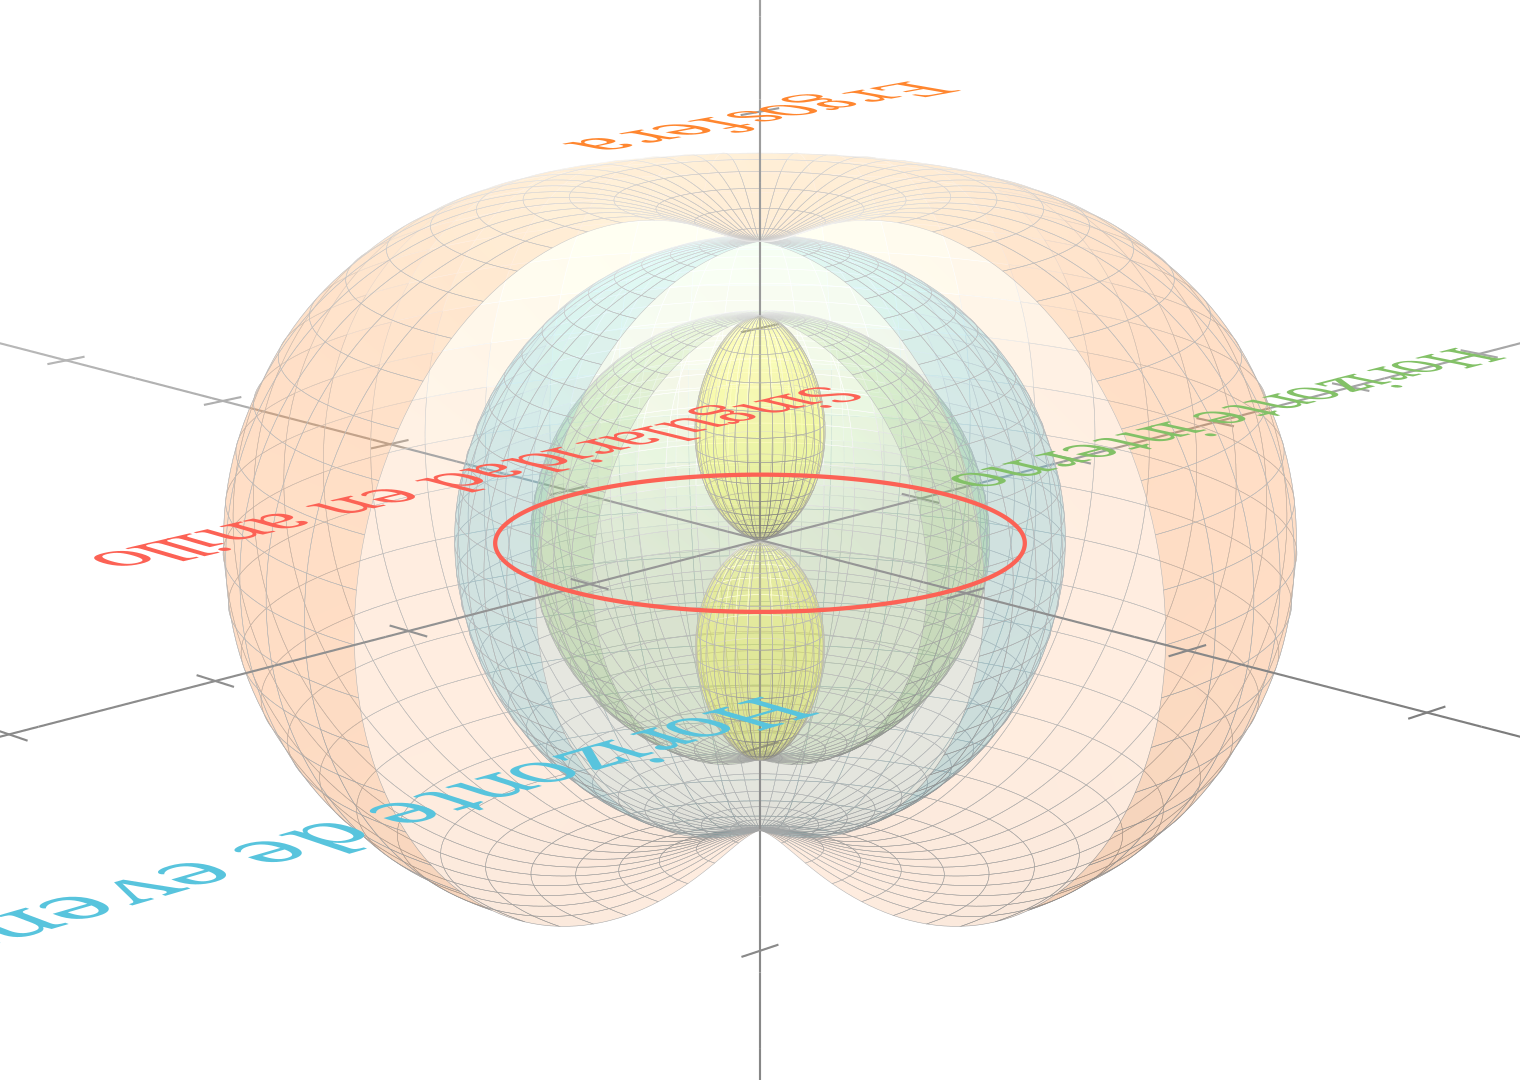
\includegraphics[width=0.95\textwidth]{AgujerosNegros/kerr/media/images/kerr_BH_regions_ManimCE_v0.19.0.png}
        \end{center}
        \caption{Representación tridimensional de las superficies que delimitan las regiones en el espacio-tiempo de Kerr, con parámetros $m=1$ y $a=0.99$.}
        \label{fig:kerr_BH_regions}
    \end{small}
\end{figure}

\section{Geodésicas en Kerr}
Para el análisis de las geodésicas en Kerr podemos hacerlo directamente con la ecuación de geodésica y calculando los símbolos de Christoffel, pero este enfoque a pesar de que es siempre valido para esta métrica no diagonal implica un coste computacional mas grande, además de que es  mas conveniente y un enfoque habitual para esta métrica usar el formalismo de cantidades conservadas usando los vectores de Killing, y el formalismo de Hamilton-Jacobi, este enfoque permite la separabilidad de las ecuaciones de movimiento este enfoque fue introducido por \cite{carter-1968}.
En la sección \ref{chap:hamilton} se discute el formalismo de Hamilton-Jacobi y la ecuación de geodésica (\ref{eq:geodesicHamiltonJacobi}) que es válida para cualquier métrica, por lo que la usaremos directamente en la métrica de Kerr.

%%%%%%%%%%%%%%%%%%%%%%%%%%%%%%%%%%%%
\subsection{Vectores de Killing en Kerr}
La métrica de Kerr tiene 2 vectores de Killing que nos llaman la atención, uno temporal y otro axial, esto se puede intuir al observar la métrica (\ref{eq:covariantKerrMetric}) y notar que no depende de las coordenadas $t$ y $\varphi$ (Nótese que esta esta expresada en una base esférica).Alternativamente se puede resolver la ecuación de Killing(\ref{eq:killing}) y comprobar que existen dos soluciones linealmente independientes $\v{e_{ct}}$ y $\v{e_\varphi}$.

Usaremos estos vectores de Killing para construir cantidades conservadas a lo largo de las geodésicas usando el resultado de la ecuación (\ref{eq:KillingCantidadConservada}) que usa un Killing y el cuatro-vector de velocidad, considerando primero el Killing axial $\v{\xi}=\v{e_\varphi}$

\begin{align}
    \d{(\xi_\mu U^\mu)}{\lambda} & = \d{(g_{\mu\nu} \xi^\nu U^\mu)}{\lambda}                               \\
                                 & =\d{(g_{\mu\varphi}  U^\mu)}{\lambda}                                   \\
                                 & =\d{(g_{ ct \varphi}  U^{ct} + g_{\varphi\varphi}  U^\varphi)}{\lambda} \\
                                 & =0 .
\end{align}
La cantidad $g_{ ct \varphi}  U^{ct} + g_{\varphi\varphi}  U^\varphi$, o de forma equivalente $g_{ ct \varphi}  p^{ct} + g_{\varphi\varphi}  p^\varphi$ es constante a lo largo de las geodésicas, y representa el componente del momento angular del cuatro-momento de una partícula en la dirección azimutal $\v{e_\varphi}$, o bien su componente en el eje z cartesiano.

\begin{equation}
    \begin{aligned}
        \tilde{L_z}  \equiv\frac{L_z}{\mu} = & g_{ ct \varphi}  U^{ct} + g_{\varphi\varphi}  U^\varphi                                    \\
                                             & =- \fr{2 mar \sin^2\theta}{\rho^2}   U^{ct} + \fr{\Sigma \sin^2\theta}{\rho^2}  U^\varphi,
    \end{aligned}
\end{equation}
es mas sencillo notar esto al recobrar la definición clásica de momento angular cuando  $a=0$ el termino  $\fr{\Sigma \sin^2\theta}{\rho^2} U^\varphi$ se convierte en el momento angular por unidad de masa clásico $L_z= r^2 sin^2\theta U^\varphi$ respecto al eje $z$ de la partícula, solo que aquí tenemos una corrección dada la naturaleza rotacional del espacio-tiempo.

Análogamente para el vector de Killing $\v{\xi} = \v{e_{ct}}$ la cantidad conservada es energía por unidad de masa

\begin{equation}
    \begin{aligned}
        - \frac{\tilde{E}}{c} \equiv -\frac{E}{\mu c} & = g_{ ct ct}   U^{ct}  +g_{ ct \varphi}  U^\varphi                                              \\
                                                      & =   -\left(1-\fr{2 mr}{\rho^2}\right)  U^{ct} -    \fr{2 mar \sin^2\theta}{\rho^2}    U^\varphi
    \end{aligned}
\end{equation}
estas cantidades conservadas van bajo la suposición de que estamos trabajando con partículas masivas, para una descipción de fotones se debe de usar el cuatro-momento $p^\mu$ en lugar del cuatro-velocidad $U^\mu$, y las cantidades conservadas  se reescriben en términos de $p^\mu$ es decir ($\v{\xi}_\mu p^\mu$) tal que
\begin{align}
    L_z         & =- \fr{2 mar \sin^2\theta}{\rho^2}   p^{ct} + \fr{\Sigma \sin^2\theta}{\rho^2}  p^\varphi,     \\
    - \fr{E}{c} & =  - \left(1-\fr{2 mr}{\rho^2}\right)  p^{ct} -   \fr{2 mar \sin^2\theta}{\rho^2}    p^\varphi
\end{align}



\subsection{Arrastre de marcos inerciales}
Una vez que ya tenemos las ecuaciones de la geodésica en Kerr, podemos analizar algunos efectos interesantes que surgen debido a la rotación del espacio tiempo, para la medición de los efectos del arrastre de marcos inerciales en la métrica de Kerr, se propone la cantidad

\begin{equation}
    \Omega \equiv \fr{d \varphi}{d t}=\fr{U^{\varphi}}{U^t}.
\end{equation}

Un observador estacionario que mantenga una posición fija en $r,\theta$ tendrá su cuadrivelocidad dada por  $U^\mu=\left(U^t, 0,0, U^{\varphi}\right)$ y el elemento de linea no tendrá las componentes $dr$ y $d\theta$.
Para que la trayectoria sea físicamente posible $\left(d s^2<0\right)$ debe cumplirse

\begin{equation}
    d s^2=g_{t t}dt^2+2 g_{t \varphi} dtd\varphi+g_{\varphi \varphi}d\varphi^2<0.
\end{equation}
Si consideramos que este observador es de tipo ZAMO  (Zero Angular Momentum Observer) es un observador con masa que no tiene momento angular propio con respecto al eje de rotación, la cantidad conservada $L=0$ implica que
\begin{equation}
    \begin{aligned}
        \Omega & =\fr{U^{\varphi}}{U^t} = \fr{ - g_{t \varphi}}{g_{\varphi \varphi}}                  \\
               & = \fr{ \fr{2a c mr \sin^2\theta}{\rho^2}}{\fr{\Sigma \sin^2\theta}{\rho^2}}          \\
               & = \fr{2a c mr}{\Sigma}                                                               \\
               & = \fr{2a c m r}{\left(r^2+a^2\right)^2-a^2\left(r^2-2 m r+a^2\right) \sin ^2 \theta}
    \end{aligned}
\end{equation}

%%%%%%%%%%%%%%%%%%%%%%%%%%%%%%%%%%%%%%%%%%%%%%%%%%%%%%%%%%%%%%%%%
%%%%%%%%%%%%%%%%%%%%%%%%%%%%%%%%%%%%%%%%%%%%%%%%%%%%%%%%%%%%%%%%%
\subsection{Geodésicas por Hamilton Jacobi}
En la sección \ref{chap:hamilton} se dedujo la ecuación para una geodésica en cualquier espacio-tiempo (\ref{eq:geodesicHamiltonJacobi}), la única modificación que le haremos es bautizar la masa de la partícula como $\mu$ esto para hacer una distinción  entre la masa del agujero negro, y la de la partícula que no genera deformación y se mueva por una trayectoria, de forma que en este formalismo la ecuación queda
\begin{equation}
    g^{\mu \nu} \partial_\mu S \partial_\nu S=-\mu^2c^2
    \label{eq:KerrHJ}
\end{equation}

donde por simplicidad tomaremos $\mu=1$ para partículas masivas y $\mu=0$ para fotones.
Aprovechamos las simetrías en $t$ y $\varphi$ e imponemos el ansatz separable
\begin{equation}
    S(t, r, \theta, \varphi, \lambda)=-(E/c) t+{L_z} \varphi+S_r(r)+S_\theta(\theta)+\fr{1}{2} \mu c^2\lambda.
\end{equation}
Entonces
\begin{equation}
    \partial_t S=-(E/c), \quad \partial_{\varphi} S={L_z}, \quad \partial_r S=S_r^{\prime}(r), \quad \partial_\theta S=S_\theta^{\prime}(\theta)
\end{equation}
Sustituiremos estas derivadas en la ecuación $\mathrm{H}-\mathrm{J}$ (\ref{eq:KerrHJ}).


\begin{equation}
    \begin{aligned}
        g^{\mu \nu} \partial_\mu S \partial_\nu S= & g^{t t}\left(\partial_t S\right)^2+2 g^{t \varphi}\left(\partial_t S\right)\left(\partial_{\varphi} S\right)+g^{\varphi \varphi}\left(\partial_{\varphi} S\right)^2 \\
                                                   & \quad +g^{r r}\left(S_r^{\prime}\right)^2+g^{\theta \theta}\left(S_\theta^{\prime}\right)^2                                                                         \\
        =                                          & g^{r r}\left(S_r^{\prime}\right)^2+g^{\theta \theta}\left(S_\theta^{\prime}\right)^2 +g^{t t} (E/c)^2-2 g^{t \varphi} (E/c) {L_z}+g^{\varphi \varphi} {L_z}^2.
    \end{aligned}
\end{equation}
Multiplicamos por $\rho^2$ y usamos $g^{r r} \rho^2=\Delta$ y $g^{\theta \theta} \rho^2=1$
\begin{equation}
    \begin{aligned}
        -\mu^2 c^2 \rho^2                           & =\rho^2 \left(g^{r r}\left(S_r^{\prime}\right)^2+g^{\theta \theta}\left(S_\theta^{\prime}\right)^2 +g^{t t} (E/c)^2-2 g^{t \varphi} (E/c) {L_z}+g^{\varphi \varphi} {L_z}^2\right) \\
        -\mu^2 c^2 r^2-\mu^2 c^2 a^2 \cos ^2 \theta & = \Delta \left(S_r^{\prime}\right)^2+1\left(S_\theta^{\prime}\right)^2  - \fr{\Sigma}{\Delta}(E/c)^2+\fr{4 a m r (E/c){L_z}}{\Delta }                                              \\
                                                    & \qquad+ \fr{ (\Delta-a^2 \sin ^2 \theta){L_z}^2 }{\Delta  \sin^{2}{\left(\theta \right)}}                                                                                          \\
                                                    & = \Delta \left(S_r^{\prime}\right)^2+\left(S_\theta^{\prime}\right)^2  - \fr{\left(\left(r^2+a^2\right)^2-a^2 \Delta \sin ^2 \theta \right)}{\Delta}(E/c)^2                        \\
                                                    & \qquad+\fr{4 a m r (E/c){L_z}}{\Delta }  + \fr{{L_z}^2}{\sin^{2}{\left(\theta \right)}} - \fr{a^2 {L_z}^2}{\Delta}                                                                 \\
                                                    & = \Delta \left(S_r^{\prime}\right)^2+\left(S_\theta^{\prime}\right)^2  - \fr{\left(r^2+a^2\right)^2}{\Delta}(E/c)^2 +a^2  \sin ^2 (\theta)(E/c)^2                                  \\
                                                    & \qquad+\fr{4 a m r (E/c){L_z}}{\Delta }  + \fr{{L_z}^2}{\sin^{2}{\left(\theta \right)}} - \fr{a^2 {L_z}^2}{\Delta}                                                                 \\
    \end{aligned}
\end{equation}
separando la ecuación en bloques de dependencia radial y angular
\begin{equation}
    \begin{aligned}
        \left[\Delta\left(S_r^{\prime}\right)^2-\frac{\left(r^2+a^2\right)^2 (E/c)^2-4 a m r (E/c) {L_z}+a^2 {L_z}^2}{\Delta}+\mu^2 c^2 r^2\right] \\
        +\left[\left(S_\theta^{\prime}\right)^2+a^2 (E/c)^2 \sin ^2 \theta+\frac{{L_z}^2}{\sin ^2 \theta}+\mu^2 c^2 a^2 \cos ^2 \theta\right] = 0
    \end{aligned}
\end{equation}
Se obtiene una ecuación separable, en la cual la única forma en que la suma de una función de $r$ y una función de $\theta$ puede ser cero para todos los valores de $r$ y $\theta$ es si ambas funciones son iguales a una constante con signo opuesto la denotaremos como $\mathcal{K}$.

$$
    \begin{array}{c}
        \text { Parte radial }=\mathcal{K} \\
        \text { Parte angular }=-\mathcal{K}
    \end{array}
$$
El desarrollo de la parte angular es el siguiente
\begin{align}
    \begin{aligned}
        \left[\left(S_\theta^{\prime}\right)^2+a^2 (E/c)^2 \sin ^2 \theta+\frac{{L_z}^2}{\sin ^2 \theta}+\mu^2 c^2 a^2 \cos ^2 \theta\right] & = -\mathcal{K} \\
        \left(S_\theta^{\prime}\right)^2+a^2 (E/c)^2 (1- \cos^2 \theta)+\frac{{L_z}^2}{\sin ^2 \theta}+\mu^2 c^2 a^2 \cos ^2 \theta          & = -\mathcal{K} \\
        \left(S_\theta^{\prime}\right)^2+a^2 (E/c)^2 - a^2 (E/c)^2 \cos^2 \theta+\frac{{L_z}^2}{\sin ^2 \theta}+\mu^2 c^2 a^2 \cos ^2 \theta & = -\mathcal{K} \\
        \left(S_\theta^{\prime}\right)^2+a^2 (E/c)^2+\frac{{L_z}^2}{\sin ^2 \theta}+(\mu^2 c^2 a^2 - a^2 (E/c)^2) \cos ^2 \theta             & = -\mathcal{K} \\
    \end{aligned}
\end{align}
Usamos la identidad trigonométrica $1 / \sin ^2 \theta=1+\cot ^2 \theta=1+\cos ^2 \theta / \sin ^2 \theta$.
\begin{equation}
    \begin{aligned}
        \left(S_\theta^{\prime}\right)^2+a^2 (E/c)^2+{L_z}^2+\frac{\cos^2 \theta {L_z}^2}{\sin ^2 \theta}+(\mu^2 c^2 a^2 - a^2 (E/c)^2) \cos ^2 \theta & = -\mathcal{K}                                    \\
        \left(S_\theta^{\prime}\right)^2+\left(\frac{ {L_z}^2}{\sin ^2 \theta}+a^2(\mu^2 c^2  -  (E/c)^2) \right)\cos ^2 \theta                        & = -(a^2 (E/c)^2+{L_z}^2+\mathcal{K}) =\mathcal{Q} \\
    \end{aligned}
\end{equation}
Aquí $\mathcal{Q}$ es la constante de Carter (introducida en \cite{carter-1968}), que junto con $(E/c)$ y ${L_z}$ son las tres cantidades conservadas que permiten la integrabilidad completa de las geodésicas en Kerr y con eso se bautiza la función
\begin{equation}
    \left(S_\theta^{\prime}\right)^2=\mathcal{Q}-\left(\frac{{L_z}^2}{\sin ^2 \theta}+a^2\left(\mu^2 c^2-(E/c)^2\right)\right) \cos ^2 \theta \equiv \Theta(\theta) .
\end{equation}

\begin{note}
    En la parte radial se puede hacer esta simplificación en el termino

    \begin{equation}
        \begin{aligned}
            \left(r^2+a^2\right)^2 (E/c)^2-4 a m r (E/c) {L_z}+a^2 {L_z}^2 & =  \left(\left(r^2+a^2\right) (E/c) -a{L_z}\right)^2+2\left(r^2+a^2\right)(E/c)a{L_z}-4 a m r (E/c) {L_z} \\
                                                                           & =  \left(\left(r^2+a^2\right) (E/c) -a{L_z}\right)^2+2\left(\left(r^2+a^2\right)-2 m r\right)a{L_z}(E/c)  \\
                                                                           & =  \left(\left(r^2+a^2\right) (E/c) -a{L_z}\right)^2+2\Delta a{L_z}(E/c)                                  \\
        \end{aligned}
    \end{equation}
\end{note}
Desarrollando la parte radial
\begin{equation}
    \begin{aligned}
        \left[\Delta\left(S_r^{\prime}\right)^2-\frac{ \left(\left(r^2+a^2\right) (E/c) -a{L_z}\right)^2+2\Delta a{L_z}(E/c) }{\Delta}+\mu^2 c^2 r^2\right] & = \mathcal{K}                       \\
                                                                                                                                                            & = -a^2(E/c)^2 -{L_z}^2 -\mathcal{Q} \\
    \end{aligned}
\end{equation}
\begin{equation}
    \begin{aligned}
        \Delta\left(S_r^{\prime}\right)^2-\frac{ \left(\left(r^2+a^2\right) (E/c) -a{L_z}\right)^2 }{\Delta}+\mu^2 c^2 r^2 & =+2 a{L_z} (E/c) -a^2(E/c)^2 -{{L_z}_z}^2 -\mathcal{Q} \\
                                                                                                                           & = -({L_z}-a (E/c) )^2 -\mathcal{Q}                     \\
    \end{aligned}
\end{equation}
\begin{equation}
    \Delta^2\left(S_r^{\prime}\right)^2  =\left(\left(r^2+a^2\right) (E/c) -a{L_z}\right)^2- \Delta(\mu^2 c^2 r^2 +({L_z}-a (E/c) )^2 +\mathcal{Q})
\end{equation}
Acompañando a la definición que se hizo antes de $\Theta(\theta)$ definimos las funciones (las cuales son consideradas estándar  en la literatura)
\begin{align}
    \Theta(\theta ) & \equiv \mathcal{Q} - \left(\frac{ {L_z}^2}{\sin ^2 \theta}+a^2(\mu^2 c^2  -  (E/c)^2) \right)\cos ^2 \theta, \\
    P(r)            & \equiv \left(r^2+a^2\right) (E/c) -a{L_z},                                                                   \\
    R(r)            & \equiv P(r)^2- \Delta(\mu^2 c^2 r^2 +({L_z}-a (E/c) )^2 +\mathcal{Q}).
\end{align}
Tal que las ecuaciones de Hamilton-Jacobi quedan
\begin{align}
    \pd{S}{r} = S_r^{\prime}(r)              & = \pm \frac{\sqrt{R(r)}}{\Delta}, \\
    \pd{S}{\theta}=S_\theta^{\prime}(\theta) & = \pm \sqrt{\Theta(\theta )}.
\end{align}

Dentro del formalismo de Hamilton-Jacobi (véase \ref{chap:hamilton} ) se tiene que
\begin{equation}
    \frac{\partial S}{\partial x^\mu} = p_\mu = \frac{\partial {L_z}}{\partial \dot{x}^\mu} = \mu g_{\mu \nu} \d{x^\nu}{\lambda}
\end{equation}
para un despeje mas  limpio $p^\sigma = g^{\sigma \mu} p_\mu =\mu g^{\sigma \mu} g_{\mu \nu} \d{x^\nu}{\lambda} = \mu \d{x^\sigma}{\lambda}$ esto es $\d{x^\sigma}{\lambda} = g^{\sigma \mu}\pd{S}{x^\mu}$
\begin{task}
    revisar como se llega a esta ecuación y revisar las constantes
\end{task}

Creando el sistema de ecuaciones diferenciales
\begin{align}
     & \d{ct}{\lambda}  = g^{t t}\pd{S}{t} + g^{t \varphi}\pd{S}{\varphi} = g^{t t}(-(E/c)) + g^{t \varphi}({L_z}) = \fr{1}{\rho^2}\left[\fr{\Sigma}{\Delta}(E/c) - \fr{2 a m r}{\Delta} {L_z}\right]                \\
     & \d{r}{\lambda}  = g^{r r}\pd{S}{r} = g^{r r} S_r^{\prime}(r) = \fr{\Delta}{\rho^2} \left(\pm \fr{\sqrt{R(r)}}{\Delta}\right) = \pm \fr{\sqrt{R(r)}}{\rho^2}                                                   \\
     & \d{\theta}{\lambda}  = g^{\theta \theta}\pd{S}{\theta} = g^{\theta \theta} S_\theta^{\prime}(\theta) = \fr{1}{\rho^2}(\pm \sqrt{\Theta(\theta )}) = \pm \fr{\sqrt{\Theta(\theta )}}{\rho^2}                   \\
     & \begin{aligned}
           \d{\varphi}{\lambda} = g^{\varphi t}\pd{S}{t} + g^{\varphi \varphi}\pd{S}{\varphi} & = g^{\varphi t}(-(E/c)) + g^{\varphi \varphi}({L_z})                                                                     \\
                                                                                              & = \fr{1}{\rho^2}\left[\fr{2 a m r}{\Delta}(E/c) + \frac{\Delta-a^2 \sin ^2 \theta}{ \Delta \sin ^2 \theta}  {L_z}\right]
       \end{aligned}
\end{align}
\begin{note}
    Se uso la siguiente igualdad para $g^{\varphi \varphi}$:
    $$
        \frac{\rho^2-2 M r}{\rho^2 \Delta \sin ^2 \theta}=\frac{r^2+a^2 \cos ^2 \theta-2 M r}{\rho^2 \Delta \sin ^2 \theta}=\frac{\Delta-a^2 \sin ^2 \theta}{\rho^2 \Delta \sin ^2 \theta} .
    $$
\end{note}
Multiplicando por $\rho ^2$ y tomando las definiciones de $P(r)$ y $R(r)$, se obtiene las ecuaciones que comúnmente se usan para describir las geodésicas en Kerr
\begin{equation}
    \begin{aligned}
        \rho^2 \frac{d r}{d \lambda}      & = \pm \sqrt{R(r)}                                                         \\
        \rho^2 \frac{d \theta}{d \lambda} & = \pm \sqrt{\Theta(\theta)}                                               \\
        \rho^2 \frac{d \phi}{d \lambda}   & =-\left(a (E/c)-\frac{{L_z}}{\sin ^2 \theta}\right)+\frac{a}{\Delta} P(r) \\
        \rho^2 \frac{d t}{d \lambda}      & =-a\left(a (E/c) \sin ^2 \theta-L_z\right)+\frac{r^2+a^2}{\Delta} P(r)
    \end{aligned}
\end{equation}

Si se observa las ecuaciones aun siguen acopladas por el termino $\rho^2(r,\theta)$, pero se puede hacer un cambio de variable para desacoplarlas (un nuevo parámetro de la trayectoria no físico) , $\gamma$, de la siguiente manera:
\begin{equation}
    d \gamma \equiv \frac{d \lambda}{\rho^2} \quad \Longrightarrow \quad \frac{d}{d \gamma}=\rho^2 \frac{d}{d \lambda}
\end{equation}

Al hacer este cambio de variable en las cuatro ecuaciones de la geodésica, estas se transforman mágicamente en un sistema mucho más manejable. Las ecuaciones para $r$ y $\theta$ se desacoplan por completo:
\begin{equation}
    \begin{aligned}
        \frac{d r}{d \gamma}      & = \pm \sqrt{R(r)}                                                         \\
        \frac{d \theta}{d \gamma} & = \pm \sqrt{\Theta(\theta)}                                               \\
        \frac{d \phi}{d \gamma}   & =-\left(a (E/c)-\frac{{L_z}}{\sin ^2 \theta}\right)+\frac{a}{\Delta} P(r) \\
        \frac{d ct}{d \gamma}     & =-a\left(a (E/c) \sin ^2 \theta-L_z\right)+\frac{r^2+a^2}{\Delta} P(r)
    \end{aligned}
    \label{eq:kerr_geodesics_mino}
\end{equation}

\section{simulación de orbitas en Kerr}
De manera genérica para construir una simulación de las geodésicas en Kerr, consideremos los parámetros del agujero negro como lo son $a$ y $m$. Estos parámetros determinan la forma de la métrica y, por lo tanto, las trayectorias de las partículas que orbitan el agujero negro, y se consideran fijos.

La simulación numérica se hizo en python con las librerías de SciPy y NumPy para resolver las ecuaciones \ref{eq:kerr_geodesics_mino}, posteriormente se utilizó la librería Matplotlib para la visualización de las trayectorias.


\begin{lstlisting}[language=Python, caption= {Este es el código genérico para la simulación de geodésicas en el espacio-tiempo de Kerr, se fijaron valores para las constantes $E$ y $L_z$, posiciones iniciales para $r$, $\theta$, $\phi$ y $t$. Además se uso la constante de masa $\mu$ a 1, asi como también $c$ a 1.Posteriormente se puede usar Matplotlib para ver las trayectorias, se puede encontar el codigo completo en los anexos \ref{chap:programa_geodesicas}.}]

import numpy as np
from scipy.integrate import solve_ivp
import matplotlib.pyplot as plt

# --- Variables Globales para el Manejo de Puntos de Inflexión ---
# Guardan el signo de la velocidad para saber si la partícula va hacia adentro/afuera
# o hacia arriba/abajo.
sign_r = 1.0  # Empezamos moviéndonos hacia afuera
sign_theta = 1.0 # Empezamos moviéndonos hacia el polo norte

# Guardan el valor de la derivada anterior para ayudar a detectar el cambio de signo.
dr_dtau_prev = 0.0
dtheta_dtau_prev = 0.0


# Constantes del agujero negro
a = 0.9
m = 1.0
c = 1.0

# Constantes de la geodésica
# Estas se calclulan por separado
# Constantes de movimiento para una órbita inclinada y en precesión
E = 0.95     # Energía 
Lz = 3.0     # Momento angular axial
Q = 15.0     # Constante de Carter (alta para una gran inclinación)
mu = 1.0     # Masa de la partícula (1 para masiva, 0 para fotón)

# Condiciones iniciales [r0, theta0, phi0, t0]
r0 = 6.0*m
theta0 = np.pi / 3  # Inclinación inicial de 60 grados respecto al ecuador
phi0 = 0.0
t0 = 0.0
y0 = [r0, theta0, phi0, t0]


tau_max = 100
tau_span = [0, tau_max]

def kerr_geodesics(tau, y, m, a, E, Lz, Q):
    """
    Define el sistema de EDOs para las geodésicas de Kerr en tiempo Mino (tau).
    El vector de estado es y = [r, theta, phi, t].
    """
    global sign_r, sign_theta, dr_dtau_prev, dtheta_dtau_prev
    r, theta, phi, t = y

    # Términos auxiliares de la métrica
    Delta = r**2 - 2 * m * r + a**2


    Rr = ((r**2 + a**2) * (E/c) - a * Lz)**2 - Delta * ((mu * c * r)**2 + (Lz - a * (E/c))**2 + Q)

    # El término np.sin(theta)**2 + 1e-9 evita la división por cero en los polos.
    Th = Q - np.cos(theta)**2 * (Lz**2 / (np.sin(theta)**2 + 1e-9)+a**2 * ((mu* c)**2 - (E/c)**2))

    # Se truncan a cero valores negativos pequeños que puedan surgir de errores de precisión.
    Rr = max(Rr, 0.0)
    Th = max(Th, 0.0)

    # Detección y manejo simple de puntos de inflexión (turning points)
    # Si el potencial es casi cero y la velocidad anterior era mayor, invertimos la dirección.
    if Rr < 1e-7 and dr_dtau_prev**2 > Rr:
        sign_r *= -1
    if Th < 1e-7 and dtheta_dtau_prev**2 > Th:
        sign_theta *= -1

    # Derivadas con respecto al tiempo Mino (tau)
    dr_dtau = sign_r * np.sqrt(Rr)
    dtheta_dtau = sign_theta * np.sqrt(Th)

    # Actualizamos los valores de las derivadas para la siguiente iteración
    dr_dtau_prev = dr_dtau
    dtheta_dtau_prev = dtheta_dtau

    dphi_dtau = (Lz / (np.sin(theta)**2 + 1e-9) - a * (E/c)) + (a *((r**2 + a**2) * (E/c) - a * Lz) / Delta)

    dt_dtau = - a * (a * (E/c) * np.sin(theta)**2 - Lz) + ((r**2 + a**2) * ((r**2 + a**2) * (E/c) - a * Lz) / Delta)

    return [dr_dtau, dtheta_dtau, dphi_dtau, dt_dtau]

print("Iniciando la integración numérica...")

# Genera 2000 puntos espaciados uniformemente para una curva suave.
t_eval_points = np.linspace(tau_span[0], tau_span[1], 2000) 

# Llamada al solver de EDOs de SciPy
sol = solve_ivp(
    fun=kerr_geodesics,
    t_span=tau_span,
    y0=y0,
    args=(m, a, E, Lz, Q),
    method='Radau',      # Un método robusto para este tipo de problemas
    dense_output=True,   # Permite obtener una solución continua y suave
    rtol=1e-8,           # Tolerancia relativa para alta precisión
    atol=1e-8,           # Tolerancia absoluta
    t_eval=t_eval_points # Puntos donde se evalúa la solución
)


print("Integración completada con éxito.")


# Extraer los resultados de la solución
r, theta, phi, t = sol.y
\end{lstlisting}

En este ejemplo se propuso las cantidades $E$, $L_z$ y $\mathcal{Q}$, en un flujo de trabajo realista se propone el punto de partida  $(r_0, \theta_0, \phi_0, t_0)$, para posteriormente proponer los valores de $E$, $L_z$ y $\mathcal{Q}$ para la situación que se desee analizar (y si se desea calcular las velocidades o momentos iniciales), o bien a partir de las condiciones iniciales de posición y velocidad (o momento) de la partícula en la geodésica calcular el valor de estas constantes.

\begin{figure}[H]
    \begin{subfigure}{0.5\textwidth}
        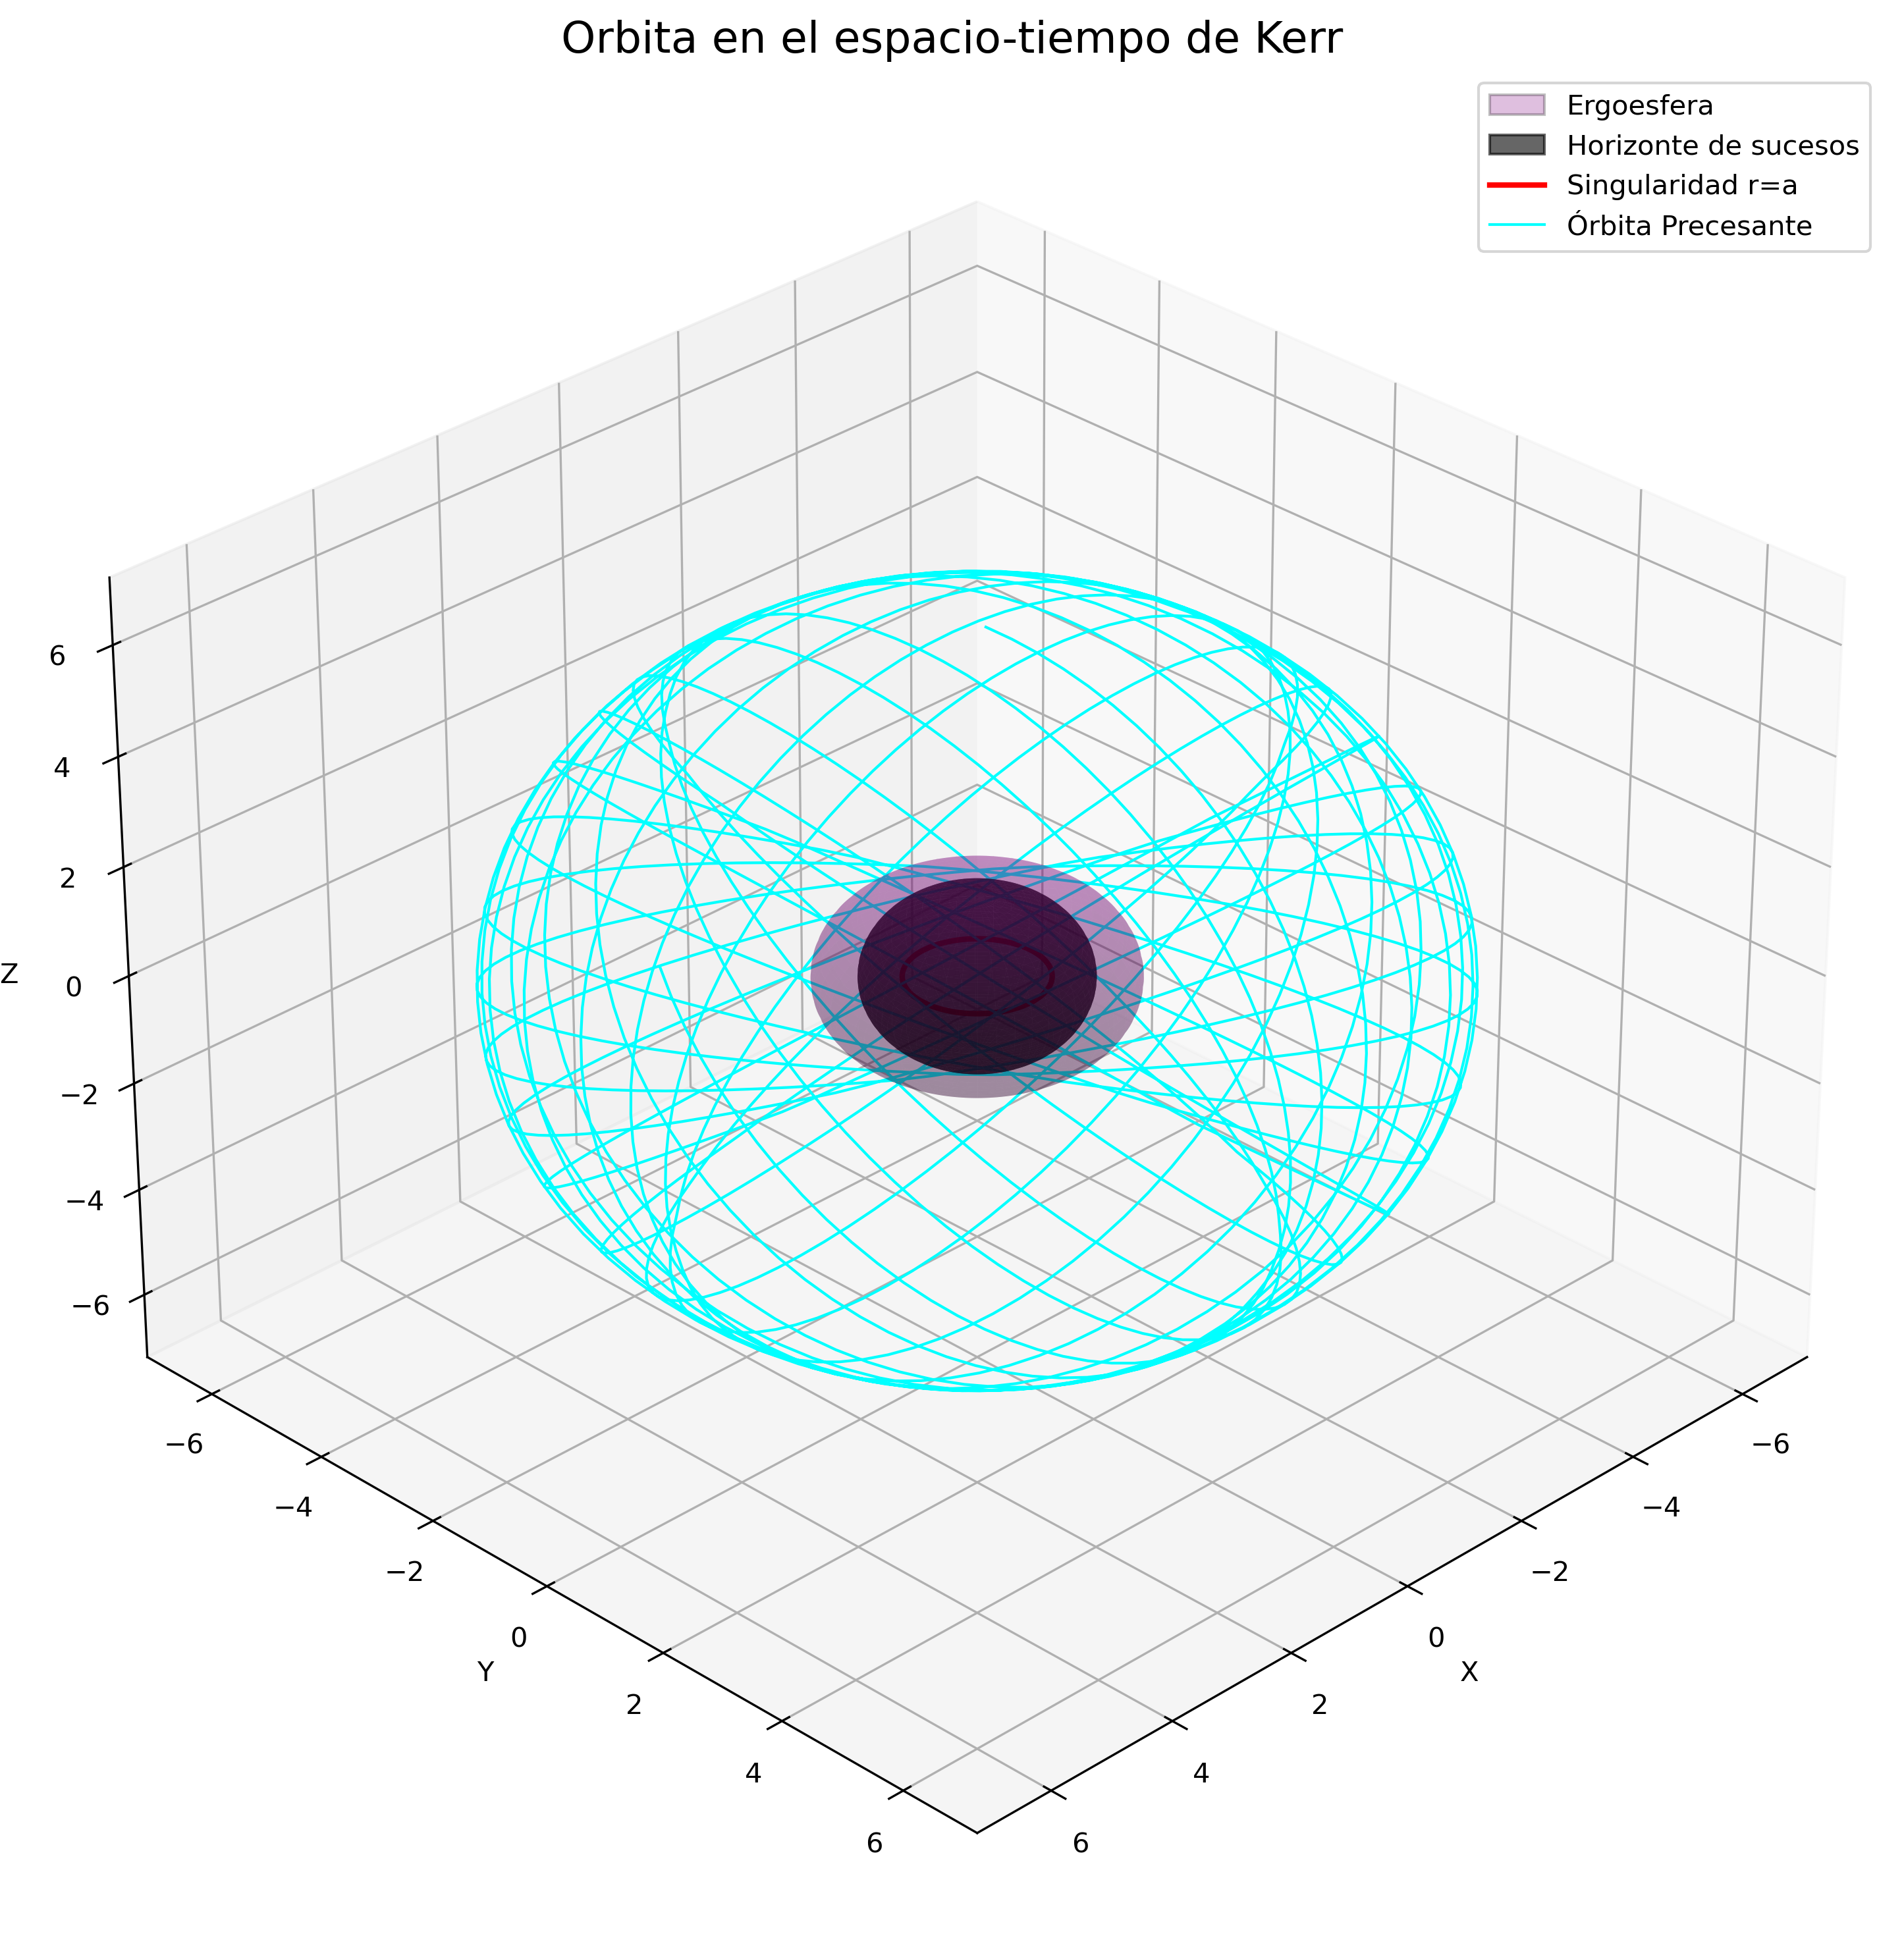
\includegraphics[width=0.9\linewidth, height=6cm]{AgujerosNegros/kerr/geodesics_plots/Geodesica1.png}
        \caption{Trayectoria de la partícula en el espacio-tiempo de Kerr}
    \end{subfigure}
    \begin{subfigure}{0.5\textwidth}
        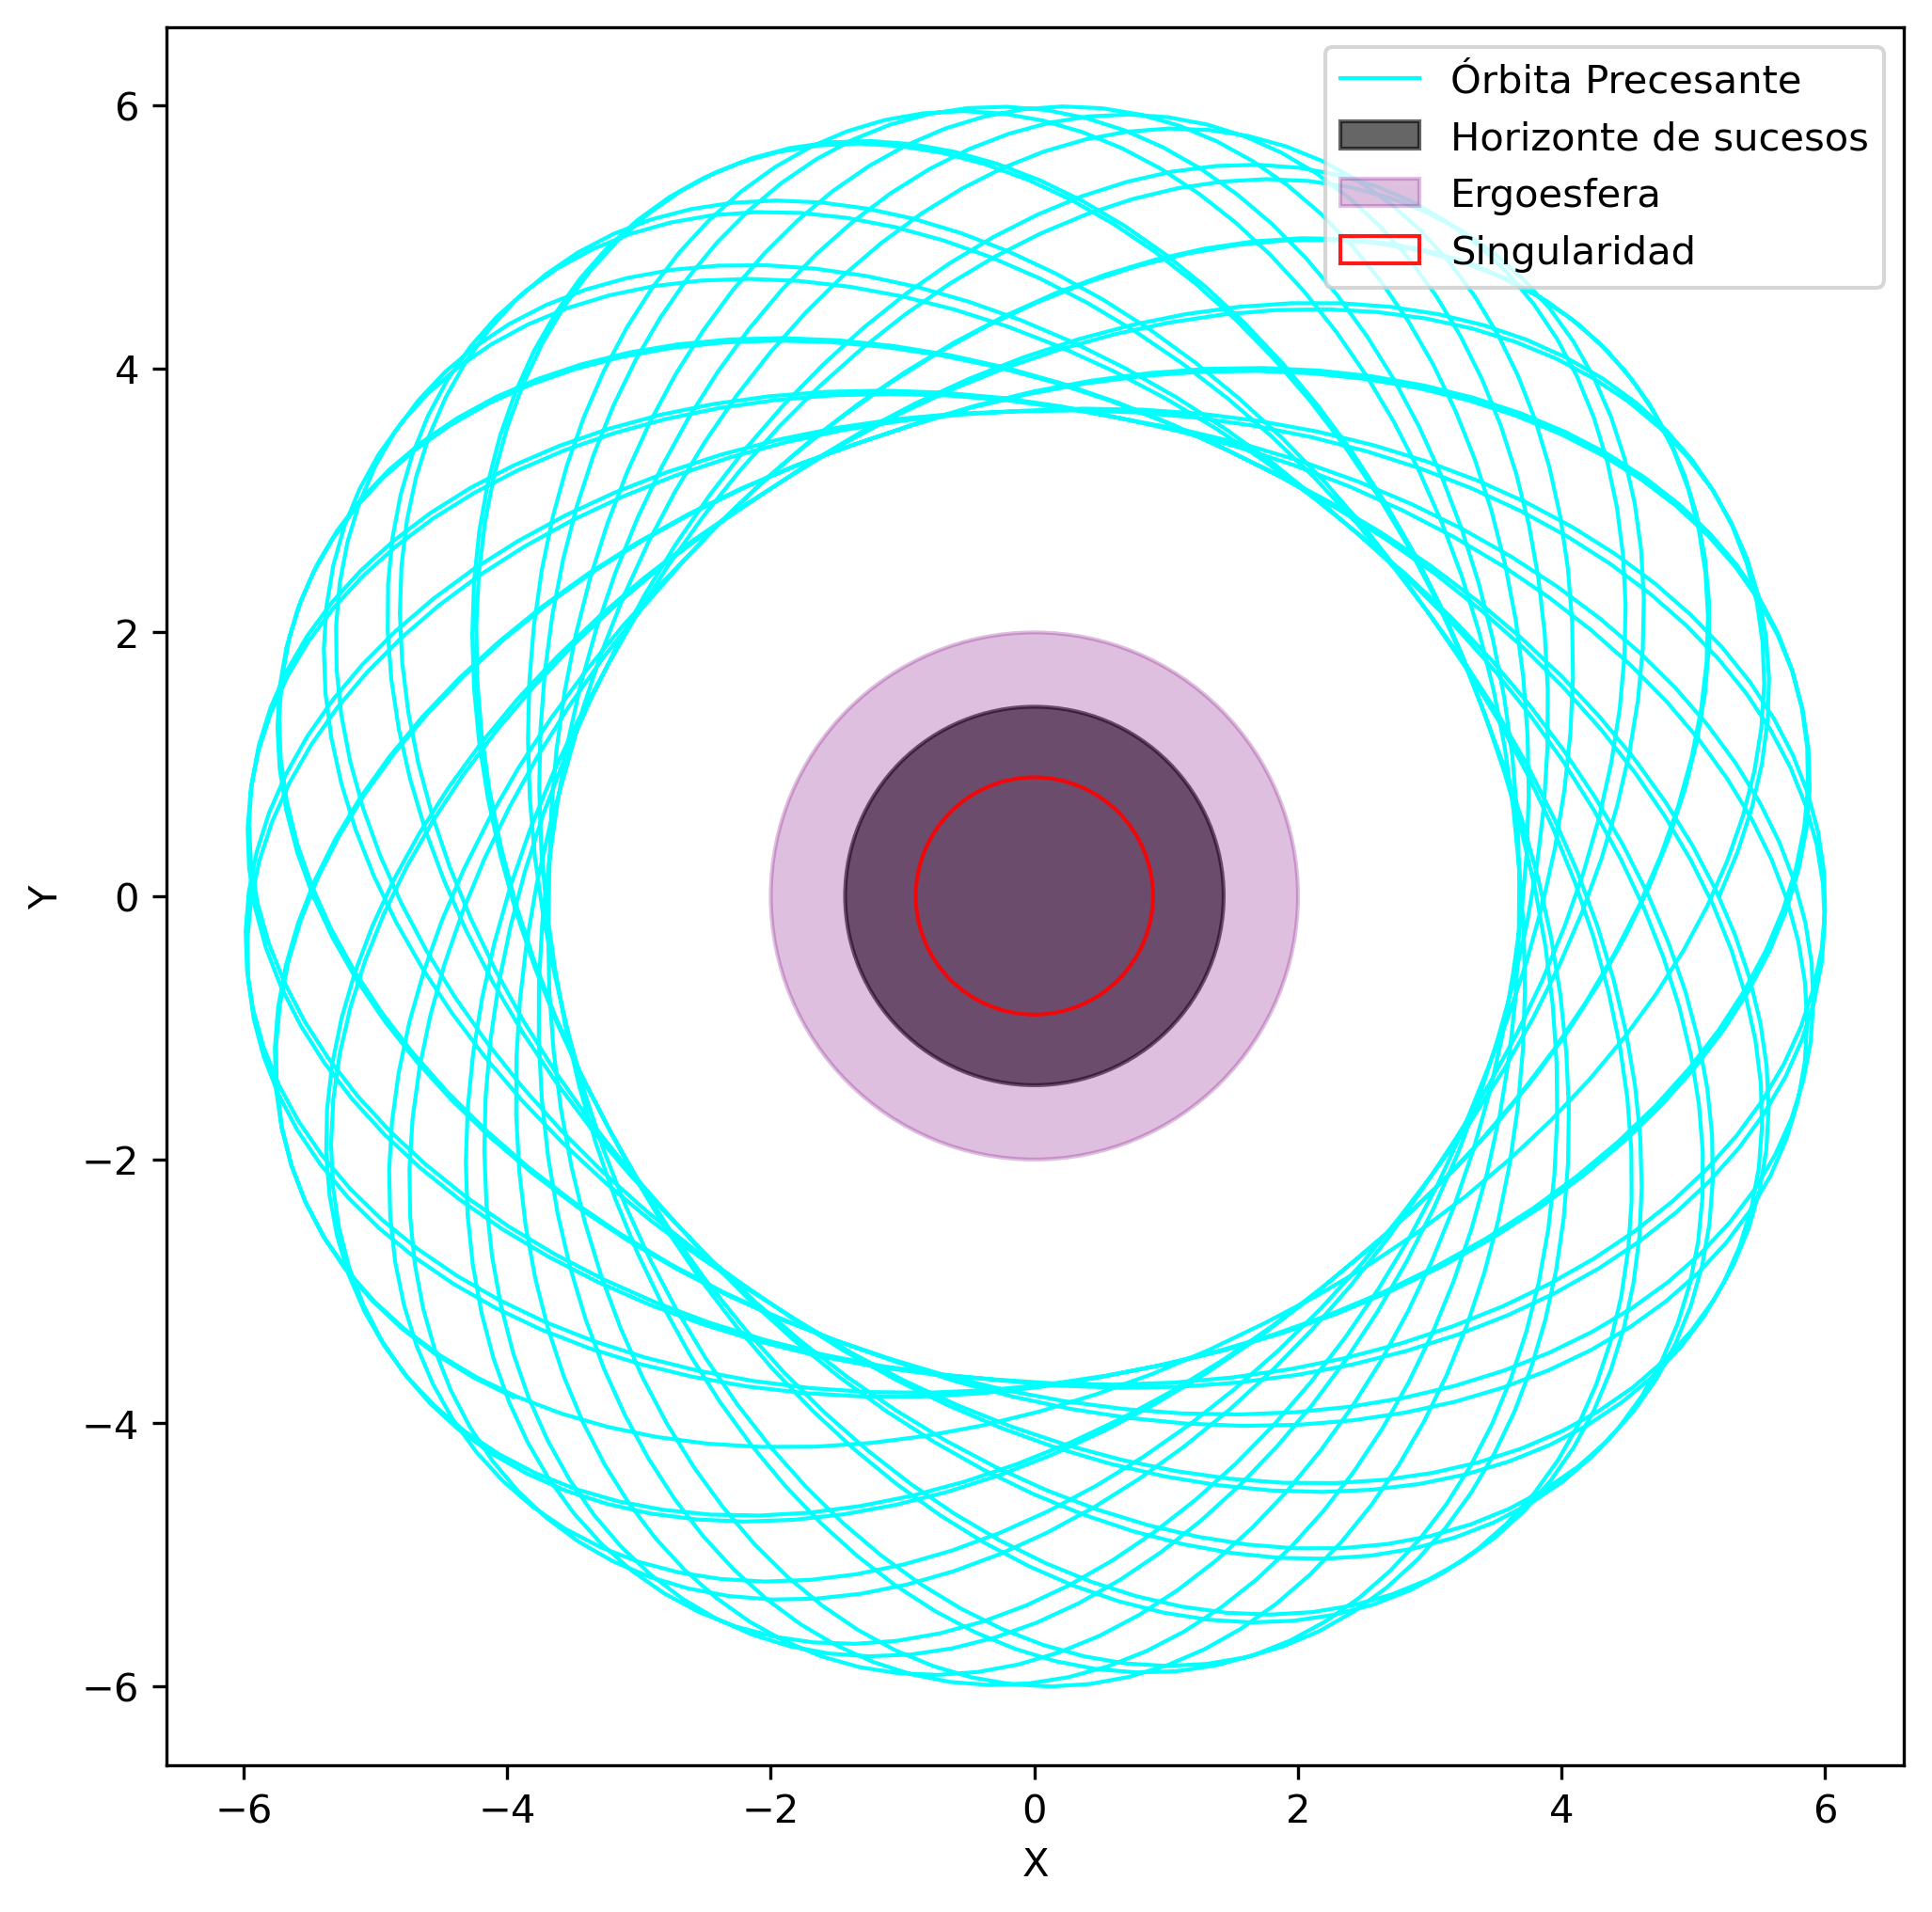
\includegraphics[width=0.9\linewidth, height=6cm]{AgujerosNegros/kerr/geodesics_plots/Geodesica1_planoxy.png}
        \caption{Trayectoria de la partícula en el plano $x-y$}
    \end{subfigure}
    \caption{Trayectoria de la partícula en el espacio-tiempo de Kerr con parámetros $a=0.9$, $m=1$, $E=0.95$, $L_z=3$ y $\mathcal{Q}=15$. La partícula inicia en $r_0=6m$, $\theta_0=\pi/3$, $\phi_0=0$ y $t_0=0$ y con $c = 1$. Se observa una órbita inclinada con precesión alrededor del agujero negro.}
\end{figure}



\subsection{El Calculo de las Constantes}
Para el calculo se fija un estado inicial $\left(r_0, \theta_0, \phi_0\right)$ y una velocidad inicial $\left(U_0^r, U_0^\theta, U_0^\phi\right)$. (La componente $U_0^t$ se fija por la condición de normalización $g_{\mu \nu} U^\mu U^\nu=-c^2$ ).
Las constantes $E$ y $L_z$ se calculan directamente a partir del cuadrivector velocidad inicial $U_0^\mu$ y la métrica $g_{\mu \nu}$ en el punto inicial:

\begin{equation}
    \begin{aligned}
        E=- c p_t= -g_{t \sigma} \mu c U_0^\sigma= -c \mu \left.\left(g_{t t} \frac{d t}{d \lambda}+g_{t \phi} \frac{d \phi}{d \lambda}\right)\right|_0 , \\
        L_z=p_\phi= g_{\phi \sigma} \mu U_0^\sigma= \mu \left.\left(g_{\phi t} \frac{d t}{d \lambda}+g_{\phi \phi} \frac{d \phi}{d \lambda}\right)\right|_0.
    \end{aligned}
    \label{eq:constantes_kerr_ELz}
\end{equation}
Una vez que se tiene $E$ y $L_z$, y conociendo la velocidad inicial $U_0^\theta=(d \theta / d \lambda)_0$, se despeja la constante de Carter $\mathcal{Q}$ de la ecuación para el movimiento en $\theta$ :


\begin{equation}
    \mathcal{Q}=\left.\left(\rho^2 \frac{d \theta}{d \lambda}\right)^2\right|_0 +\left(\frac{L_z^2}{\sin ^2 \theta_0}+a^2\left(\mu^2 c^2-(E/c)^2\right)\right) \cos ^2 \theta_0 .
\end{equation}
Aquí se puede apreciar la naturaleza de la constante, Representa la contribución del movimiento fuera del plano ecuatorial. Sus unidades corresponden a momento angular al cuadrado.

Por conveniencia matemática podemos tomar como posición inicial un punto en el ecuador $\theta_0=\pi / 2$, de esta forma la ecuación para $\mathcal{Q}$ se simplifica a
\begin{equation}
    \mathcal{Q}=\left.\left(r^2 \frac{d \theta}{d \lambda}\right)^2\right|_0  .
\end{equation}

Además podemos tomar $\phi_0=0$ y $t_0=0$ sin pérdida de generalidad, ya que la métrica es simétrica en $\phi$ y $t$, de forma que solo sera necesario definir la distancia radial $r_0$, dejando como parámetros libres las velocidades en es punto.Este proceso se automatizo con el código del anexo \ref{chap:programa_constantes_kerr}.


\subsection{Caída }
Para dar en ejemplo algebraico de como es el calculo de las constantes probaremos que es lo que sucede con una partícula que cae hacia el agujero negro. con una posición inicial en el ecuador $(r_0, \theta_0=\pi/2, \phi_0=0)$, y cuadrivector de velocidad $U^\mu = (U^t, 0, 0, 0 )$.

Dada la condición de normalización $g_{\mu \nu} U^\mu U^\nu=-c^2$

\begin{equation}
    g_{t t}\left(r_0, \frac{\pi}{2}\right)\left({U_{(0)}}^t\right)^2=-c^2
\end{equation}


\begin{equation}
    \left(1-\frac{2 m }{r_0}\right)\left({U_{(0)}}^t\right)^2=c^2
\end{equation}
\begin{equation}
    {U_{(0)}}^t = \frac{c}{\sqrt{1-\frac{2 m }{r_0}}}.
\end{equation}
Usando las relaciones (\ref{eq:constantes_kerr_ELz})

\begin{equation}
    \begin{aligned}
        E & =  \mu c \left(1-\frac{2 m }{r_0}\right)\frac{c}{\sqrt{1-\frac{2 m }{r_0}}} \\
          & = \mu c^2 \sqrt{1-\frac{2 m }{r_0}}
    \end{aligned}
\end{equation}
y
\begin{equation}
    \begin{aligned}
        L_z & = -\mu \frac{2 m a }{r_0}{U_{(0)}}^t                        \\
            & =-\mu \frac{2 m a}{r_0} \frac{c}{\sqrt{1-\frac{2 m }{r_0}}} \\
            & = -\frac{2 m \mu  a c}{ \sqrt{(r_0)^2-2 m r_0}}.
    \end{aligned}
\end{equation}
En este caso se vio el calculo de las constantes una vez que se tenga la velocidad inicial, pero tambien es posible el proceso inverso, es decir, dado un conjunto de constantes $(E, L_z, \mathcal{Q})$ y una posición inicial $(r_0, \theta_0=\pi/2, \phi_0=0)$ se puede despejar el cuadrivector de velocidad inicial $U^\mu$, esto claro depende de que se quiera estudiar, mas adelante usaremos las constantes como simples parámetros e ignoraremos cual condición de velocidades iniciales encapsulan.
Usando el programa del anexo \ref{chap:programa_constantes_kerr} con $\mu=1$,$a = 0.9$,$m=1$ se obtiene que las constantes son

\begin{align*}
    E           & = 0.816497 ,  \\
    L_z         & =  -0.367423, \\
    \mathcal{Q} & = 0.
\end{align*}

\begin{figure}[H]
    \begin{small}
        \begin{center}
            \includegraphics[width=0.95\textwidth]{AgujerosNegros/kerr/geodesics_plots/Geodesica_caida_planoxy.png}
        \end{center}
        \caption{Partícula en caída en Kerr con $\mu=1$,$a = 0.9$,$m=1$ y condiciones iniciales $(r_0=6m, \theta_0=\pi/2, \phi_0=0)$ y velocidad inicial $U^\mu = (U^t, 0, 0, 0 )$, además se tomo $c=1$.}
    \end{small}
\end{figure}

\subsection{Clasificación de geodésicas en Kerr}
El análisis de las geodésicas en Kerr es considerablemente más complejo que en Schwarzschild pero principalmente la que función que mas nos puede ayudar a clasificar las geodésicas es la función $R(r)$, que es un polinomio de cuarto grado en $r$ y depende de las tres constantes de movimiento $E, L_z$ y $\mathcal{Q}$, además de la masa y el momento angular del agujero negro, por lo que vale la pena empezar por el estudio de esta y posteriormente analizar las otras funciones involucradas en las ecuaciones de movimiento.

Toda la información sobre el movimiento radial está contenida en la ecuación

\begin{equation}
    \left(\frac{d r}{d \gamma}\right)^2=R(r)
\end{equation}



Para que una partícula pueda existir en un cierto radio $r$, la velocidad radial al cuadrado $(\mathrm{dr} / \mathrm{d} \gamma)^2$ debe ser no negativa. Esto nos da la condición fundamental para el movimiento:

\begin{equation}
    \mathbf{R}(\mathbf{r}) \geq \mathbf{0}
\end{equation}

Las regiones donde $R(r)<0$ son zonas radiales prohibidas. Los puntos donde $R(r)=0$ son los puntos de inflexión radiales (ápsides), donde la partícula invierte su movimiento radial (pasa de acercarse a alejarse, o viceversa).
varios tipos de órbitas las podemos clasificar en base a esta función $R(r)$:
\begin{itemize}
    \item Órbitas Ligadas (Bound Orbits)
          $\mathrm{R}(\mathrm{r})=0$ tiene dos raíces positivas, $r_{\text {peri }}$ (periastro) y $r_{\text {apo }}$ (apoastro), fuera del horizonte de eventos.
    \item Órbitas de Dispersión (Unbound/Scattering Orbits)
          $R(r)=\emptyset$ tiene una sola raíz positiva, $r_{\text {min }}$. La partícula viene desde el infinito, tiene suficiente energía para superar la barrera de potencial gravitacional, se acerca hasta una distancia minima $r_{\text {min }}$ y vuelve a escapar hacia el infinito. Esto describe la trayectoria de un cometa interestelar que pasa cerca del Sol y no es capturado.
    \item Órbitas de Caida (Plunge Orbits)
          Condición: $R(r)$ es positivo para todo $r$ desde un radio inicial hasta el horizonte de eventos. O bien, la raíz de $R(r)=0$ se encuentra dentro o en el horizonte de eventos.
    \item Órbitas Circulares
          Son un caso especial donde la partícula se mantiene a un radio constante. Esto ocurre en los mínimos o máximos locales del potencial efectivo. Matemáticamente, esto requiere que se cumplan dos condiciones simultáneamente en un radio $r_c$ :

          \begin{equation}
              R\left(r_c\right)=\left.0 \quad y \quad \frac{d R}{d r}\right|_{r=r_c}=0
              \label{eq:condicionesOrbitaCircular}
          \end{equation}
          - Estabilidad:
          - Si $r_c$ es un minimo local del potencial $\left(d^2 R / d r^2>0\right)$, la órbita circular es estable. Una pequeña perturbación hará que la partícula oscile alrededor de $r_c$.
          - Si $r_c$ es un máximo local $\left(d^2 R / d r^2<0\right)$, la órbita es inestable. Cualquier pequeña perturbación hará que la partícula caiga hacia el agujero negro o escape al infinito.
\end{itemize}
\subsection{Revisión de Órbitas Circulares}
El punto aquí será buscar condiciones para que una partícula se mantenga en una órbita circular alrededor del agujero negro. Esto implica encontrar un radio $r_c$ tal que las condiciones para una órbita circular se cumplan.
Como se mencionó en la ecuación (\ref{eq:condicionesOrbitaCircular}), debemos cumplir con las dos condiciones simultáneamente.



La derivada de $R(r)$ es
\begin{equation}
    R' = 4 (E/c) r P(r)-2 c^2 \mu^2 r \Delta+2(m-r)\left(Q+c^2 \mu^2 r^2+\left((E/c) a-L_z\right)^2\right),
\end{equation}
la cual es una función polinómica de $r$ de tercer grado, encontrar sus ceros es una tarea difícil, se puede recurrir a métodos numéricos o aproximaciones analíticas para obtener soluciones.
Con el uso de un software se pueden encontrar soluciones aproximadas para los ceros de $R'(r)$.

Tal que el sistema queda
\begin{equation}
    \begin{aligned}
        P(r)^2-\Delta\left(\mu^2 c^2 r^2+\left(L_z-a(E / c)\right)^2+\mathcal{Q}\right)  =                 & 0 \\
        4 (E/c) r P(r)-2 c^2 \mu^2 r \Delta+2(m-r)\left(Q+c^2 \mu^2 r^2+\left((E/c) a-L_z\right)^2\right)= & 0
    \end{aligned}
\end{equation}
dando que las la constante de carter solo representa movimiento fuera del plano ecuatorial, se puede considerar como constante, tal que podemos resolver el sistema para $E$ y $L_z$ en función de $r_c$ y un $\mathcal{Q}_c$.
Para eso usaremos un método numérico con Python
\begin{lstlisting}[language=Python, caption={Cálculo numérico de las constantes para órbitas circulares en Kerr}, label={lst:kerr_circular_orbits}]
import numpy as np
import matplotlib.pyplot as plt
from sympy import symbols, diff, lambdify
from scipy.optimize import fsolve

# ------------------------------
# 1. PARÁMETROS DE CONFIGURACIÓN
# ------------------------------
# Constantes físicas y del agujero negro
PARAMS = {
    'm': 1.0,      # Masa del agujero negro
    'a': 0.9,      # Parámetro de espín (spin)
    'mu': 1.0,     # Masa de la partícula de prueba
    'c': 1.0       # Velocidad de la luz (unidades geometrizadas)
}

# Parámetros de simulación
R_START = PARAMS['m'] + np.sqrt(PARAMS['m']**2 - PARAMS['a']**2) + 0.1  # Justo fuera del horizonte
R_END = 6.0
N_POINTS = 200
Q_VALS = [0, 5, 10] # Valores del parámetro de Carter a simular

# ------------------------------
# 2. DEFINICIÓN SIMBÓLICA (con SymPy)
# ------------------------------
r, a, m, E, Lz, Q, mu, c = symbols('r a m E L_z Q mu c', real=True)

# Ecuaciones de la geodésica de Kerr
delta = r**2 - 2*m*r + a**2
P_func = (r**2 + a**2)*E - a*Lz
R_func = P_func**2 - delta*(mu**2*r**2 + (Lz - a*E)**2 + Q)
R_prime = diff(R_func, r)

# ------------------------------
# 3. CONVERSIÓN A FUNCIONES NUMÉRICAS (con Lambdify)
# ------------------------------
# Se convierten las expresiones de SymPy en funciones de NumPy para un cálculo rápido.
VARIABLES = [E, Lz, r, Q, a, m, mu, c]
R_numeric = lambdify(VARIABLES, R_func, 'numpy')
R_prime_numeric = lambdify(VARIABLES, R_prime, 'numpy')

# ------------------------------
# 4. FUNCIÓN SOLUCIONADORA (con SciPy)
# ------------------------------
def solve_equations(initial_guess, r_val, Q_val, params):
    """
    Resuelve el sistema R=0 y R'=0 para E y Lz usando fsolve de SciPy.
    
    Args:
        initial_guess (list): Valores iniciales para [E, Lz].
        r_val (float): Valor del radio.
        Q_val (float): Valor del parámetro de Carter.
        params (dict): Diccionario con los parámetros del agujero negro.
        
    Returns:
        tuple: (E, Lz) o (nan, nan) si la solución no se encuentra.
    """
    # Función objetivo para fsolve. Debe devolver [0, 0] en la solución.
    def objective_func(variables):
        E_sol, Lz_sol = variables
        args = (r_val, Q_val, params['a'], params['m'], params['mu'], params['c'])
        
        eq1 = R_numeric(E_sol, Lz_sol, *args)
        eq2 = R_prime_numeric(E_sol, Lz_sol, *args)
        
        return [eq1, eq2]

    try:
        # fsolve es el equivalente numérico de nsolve
        solution, _, success_flag, _ = fsolve(objective_func, initial_guess, full_output=True)
        if success_flag == 1:
            return float(solution[0]), float(solution[1])
        else:
            return np.nan, np.nan
    except RuntimeError:
        # fsolve puede lanzar un error si no converge
        return np.nan, np.nan


r_consulta = 3
q_consulta = 4
E_consulta, Lz_consulta = solve_equations([0.9, 2.0], r_consulta, q_consulta, PARAMS)
print(f"Para r={r_consulta} y Q={q_consulta}, se obtiene E={E_consulta:.6f}, Lz={Lz_consulta:.6f}")
\end{lstlisting}
En los anexos \ref{chap:programa_orbitas_circulares_kerr} se encuentra una extension de este código que se uso para las siguientes gráficas que muestran las constantes $E$ y $L_z$ en función del radio de la órbita circular $r_c$ para diferentes valores de la constante de Carter $\mathcal{Q}$.

\begin{figure}[H]
    \begin{subfigure}{0.5\textwidth}
        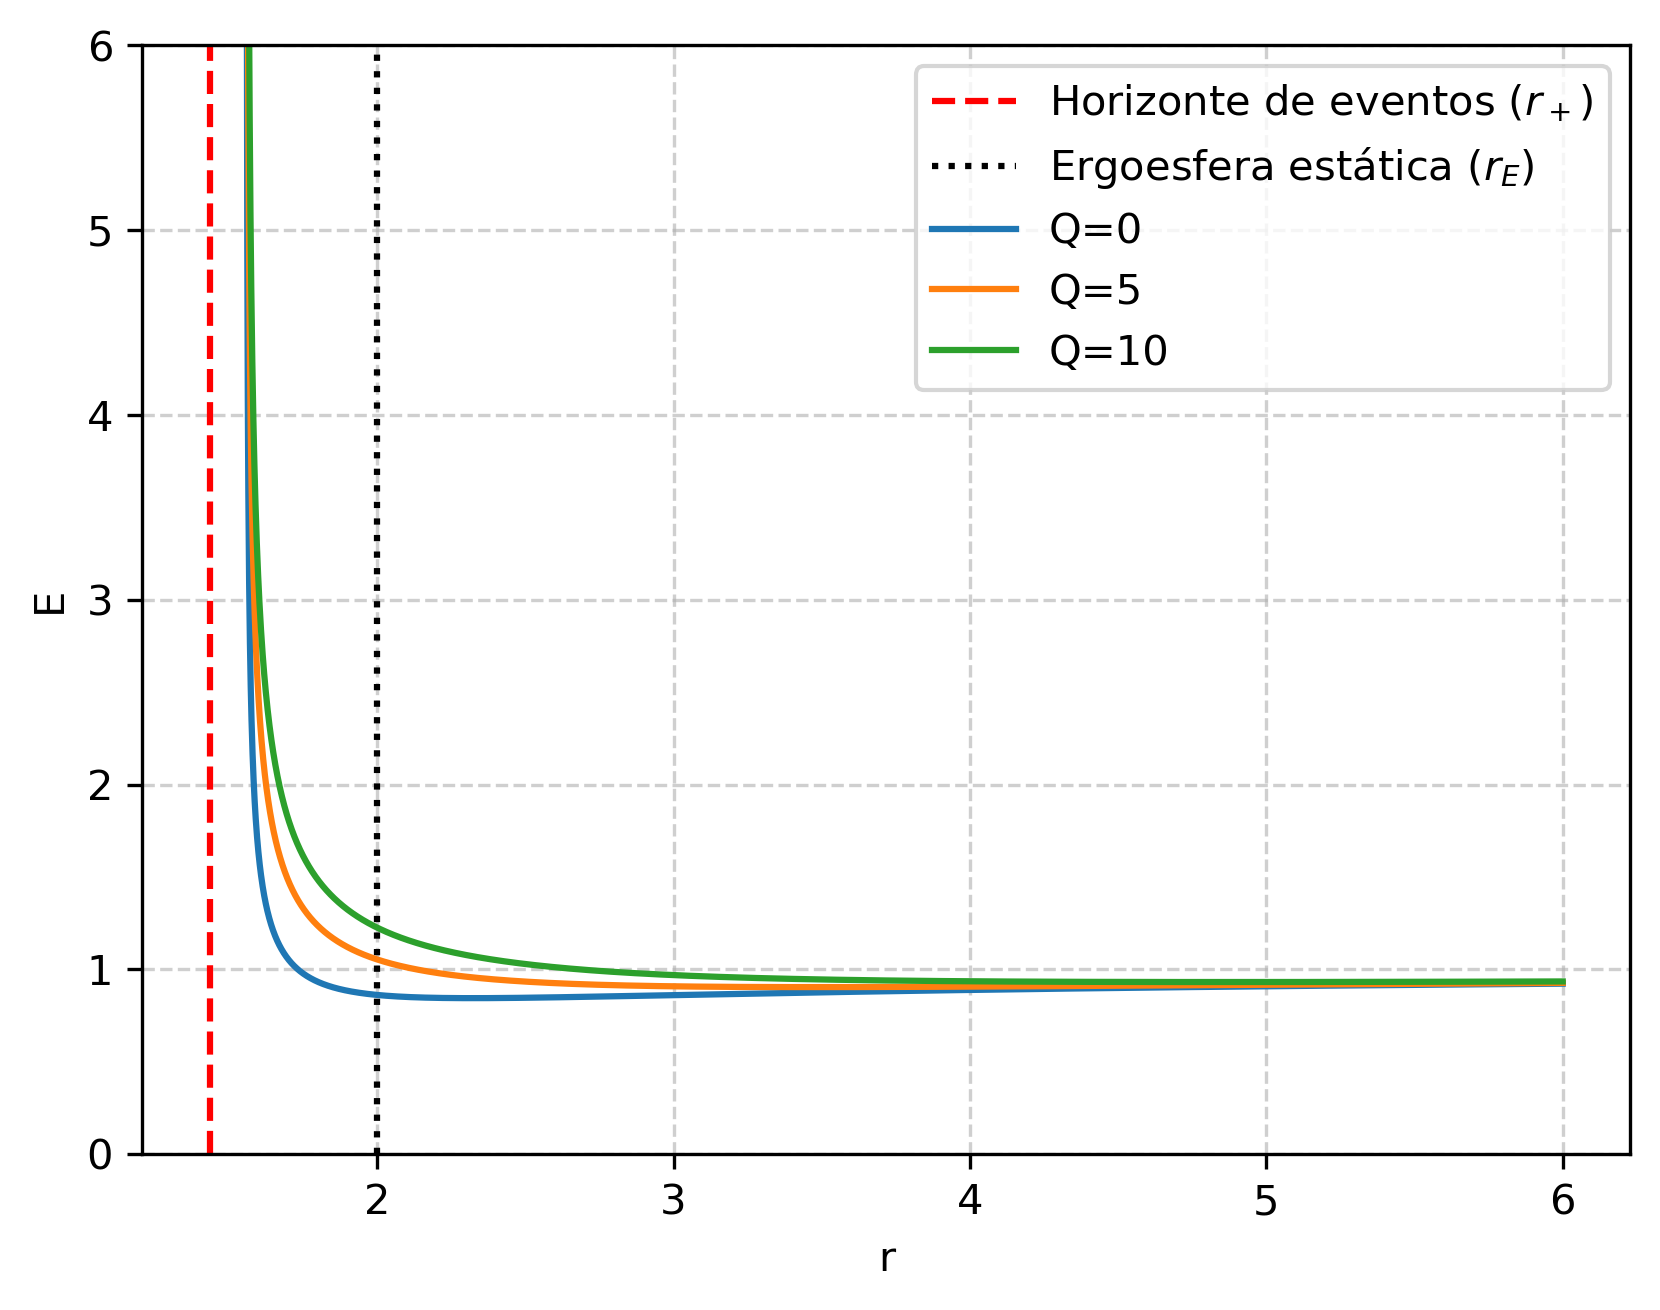
\includegraphics[width=0.9\linewidth, height=6cm]{AgujerosNegros/kerr/geodesics_plots/circular_orbits_E_vs_r.png}
        \caption{Constante de energía $E$ en función del radio $r_c$ para diferentes valores de la constante de Carter $\mathcal{Q}$.}
    \end{subfigure}
    \begin{subfigure}{0.5\textwidth}
        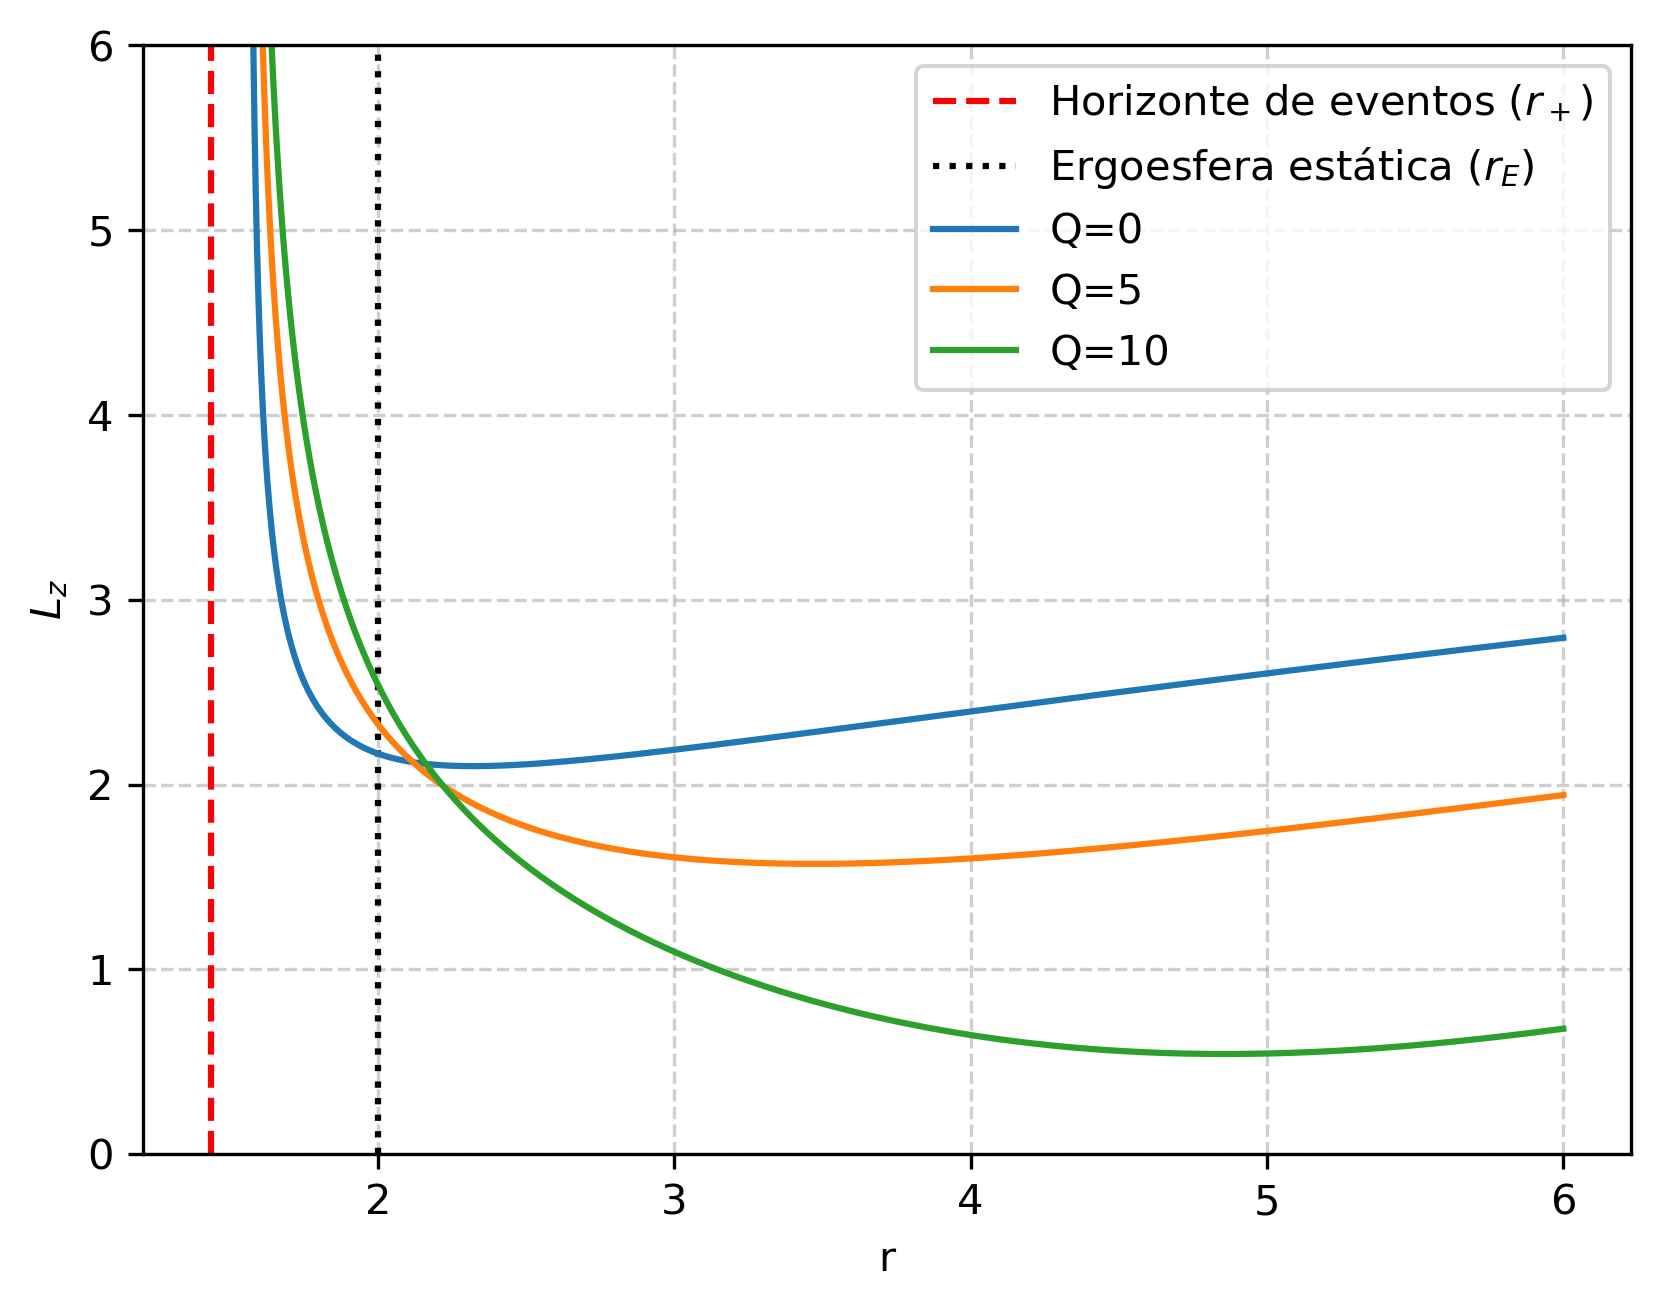
\includegraphics[width=0.9\linewidth, height=6cm]{AgujerosNegros/kerr/geodesics_plots/circular_orbits_Lz_vs_r.png}
        \caption{Constante de momento angular $L_z$ en función del radio $r_c$, para diferentes valores de la constante de Carter $\mathcal{Q}$.}
    \end{subfigure}
    \caption{Gráficas de las constantes $E$ y $L_z$ en función del radio $r_c$ para diferentes valores de la constante de Carter $\mathcal{Q}$.}
\end{figure}

\subsubsection{Simulaciones de Órbitas Circulares }
A continuación se presentan los resultados para  órbitas con $r_c = 3m$

\begin{figure}[H]

    \begin{subfigure}{0.5\textwidth}
        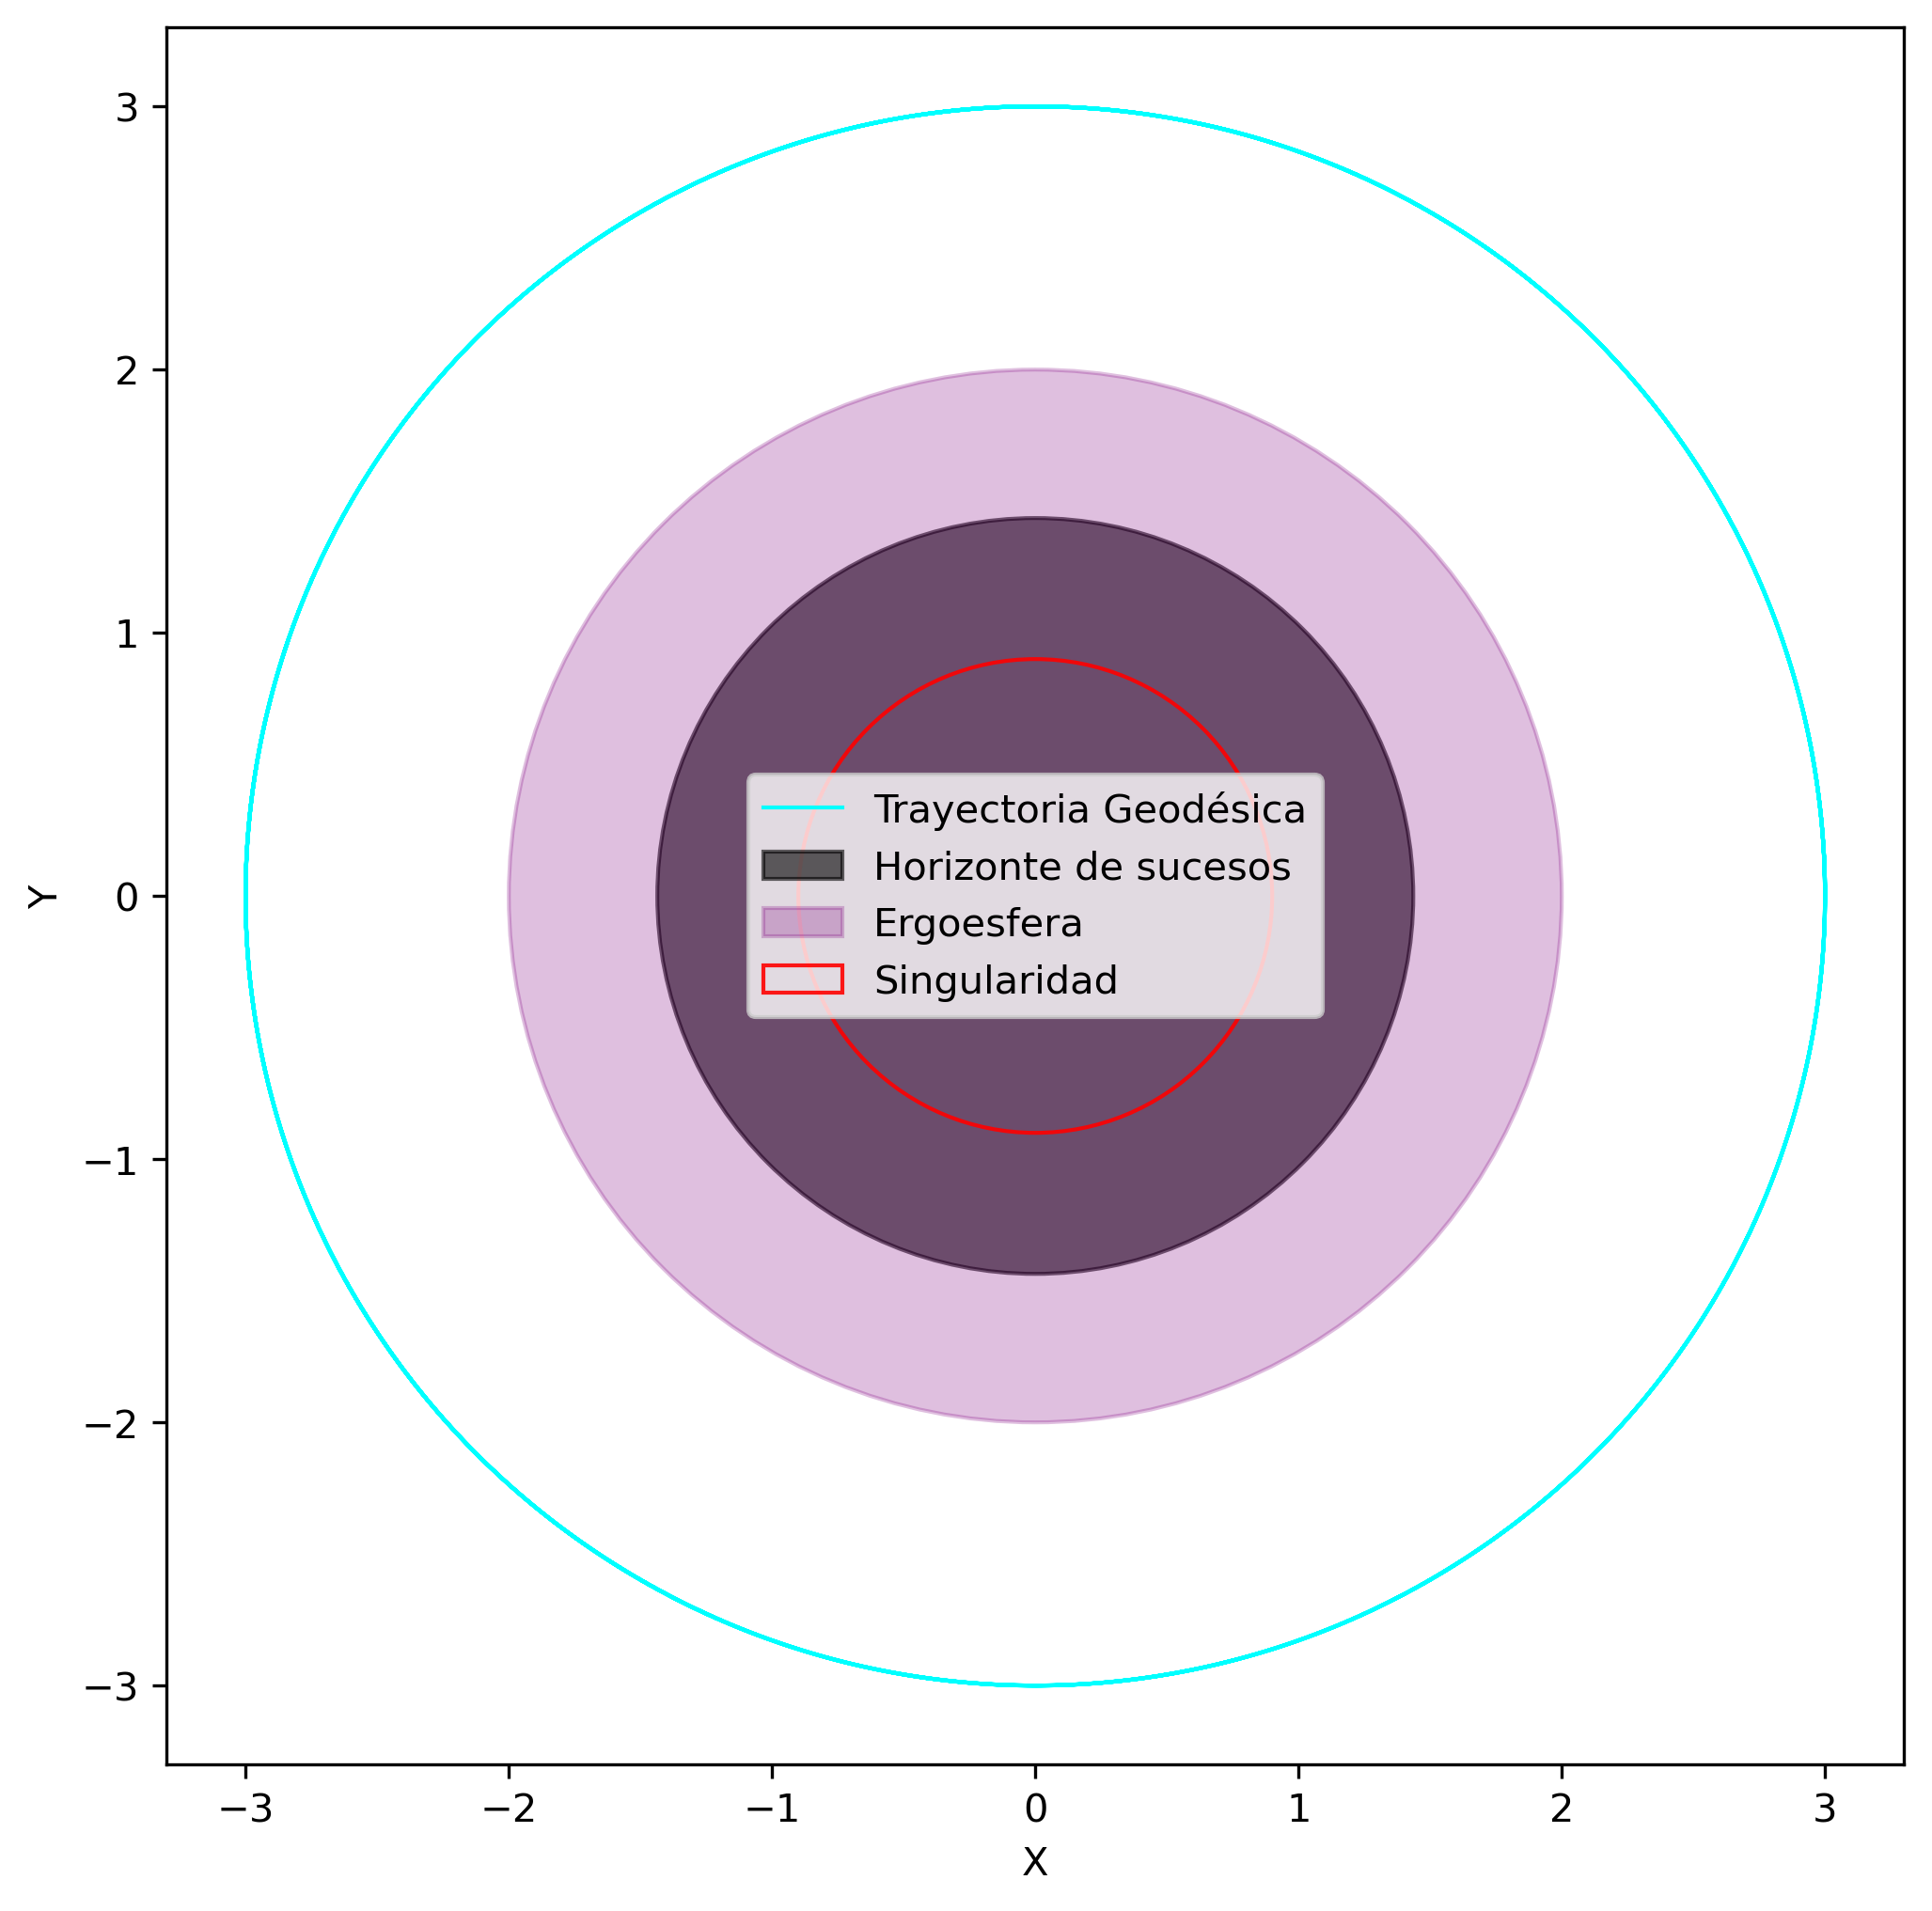
\includegraphics[width=0.9\linewidth, height=6cm]{AgujerosNegros/kerr/geodesics_plots/geodesica_circular_r3_Q0_planoxy.png}
        \caption{Para r=3 y Q=0, usa $E=0.860631$, $L_z=2.188259$}
    \end{subfigure}
    \begin{subfigure}{0.5\textwidth}
        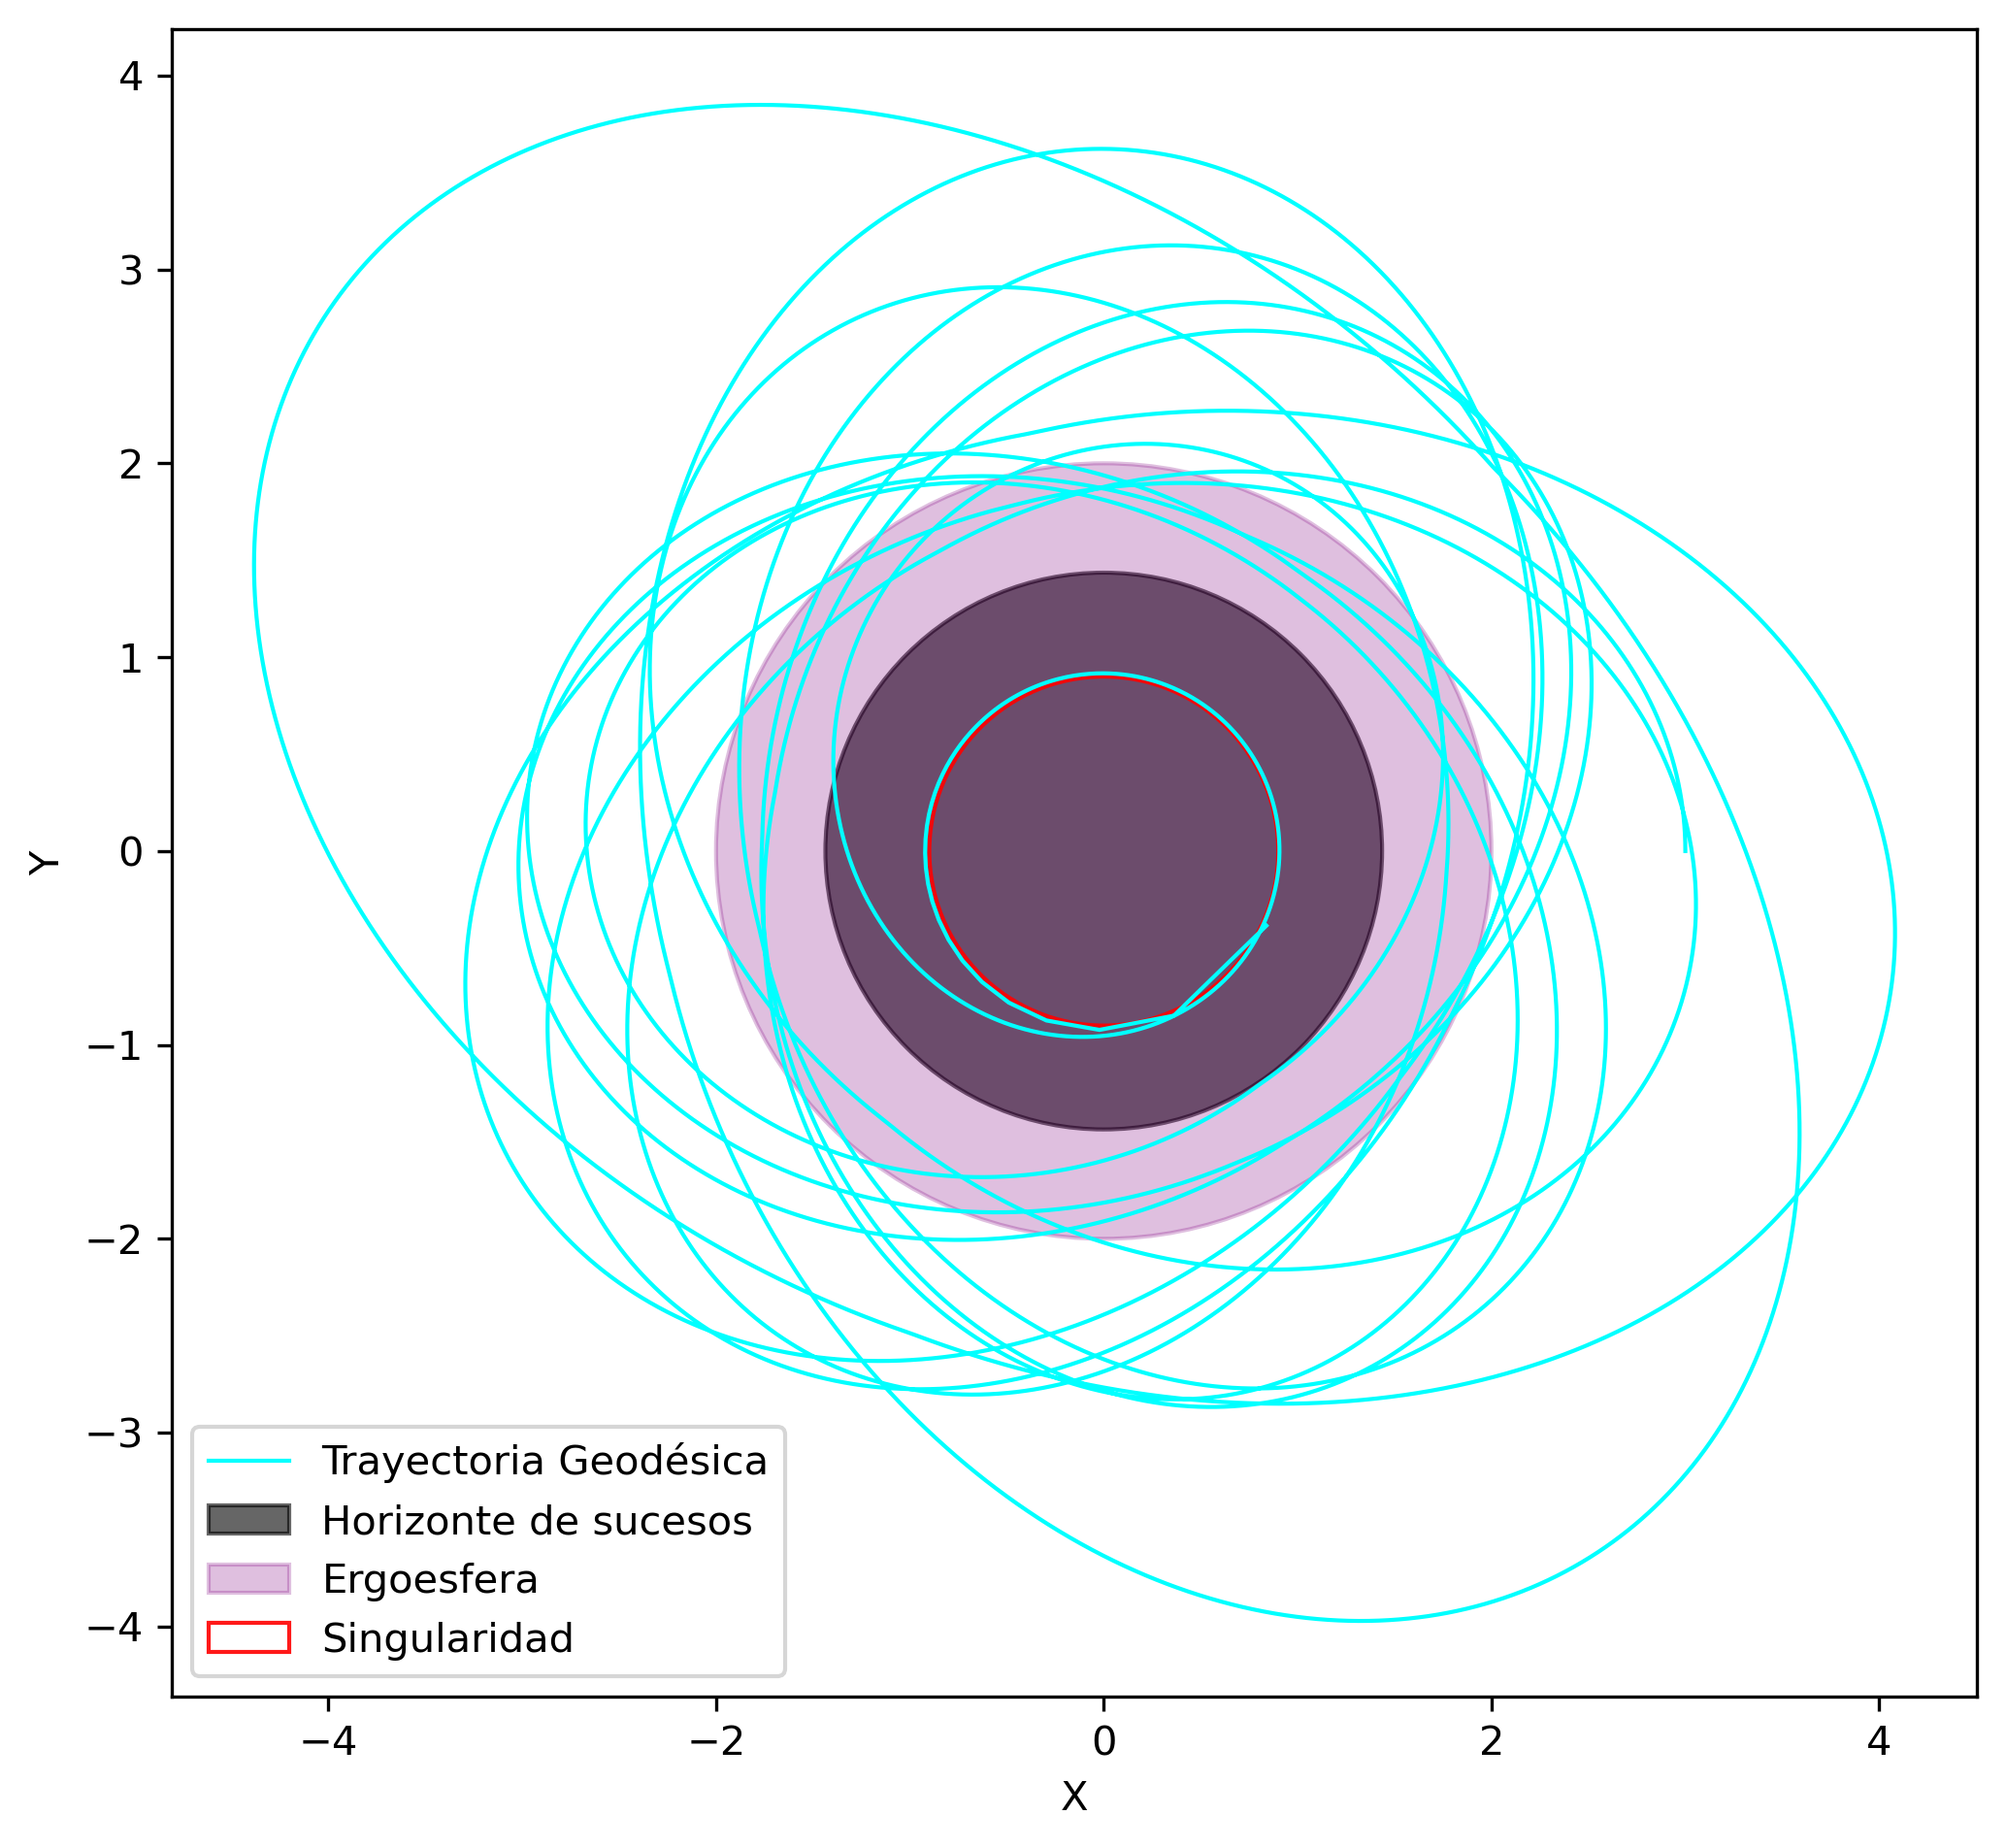
\includegraphics[width=0.9\linewidth, height=6cm]{AgujerosNegros/kerr/geodesics_plots/geodesica_circular_r3_Q5_planoxy.png}
        \caption{Para $r=3$ y $Q=5$, usa $E=0.908247$, $L_z=1.606488$}

    \end{subfigure}

    \caption{Gráficas de las constantes $E$ y $L_z$ en función del radio $r_c = 3m$ para diferentes valores de la constante de Carter $\mathcal{Q}$.}
\end{figure}

\subsubsection{Órbitas Circulares en Regiones de Interés}
Después se simuló justo en la región intermedia entre el horizonte y la ergoesfera en el ecuador
\begin{equation}
    r_c =\frac{r_E + r_+}{2}=\frac{2m + m +\sqrt{m^2-a^2}}{2}\sim 1.7179
\end{equation}

\begin{figure}[H]
    \centering
    \begin{subfigure}{0.4\textwidth}
        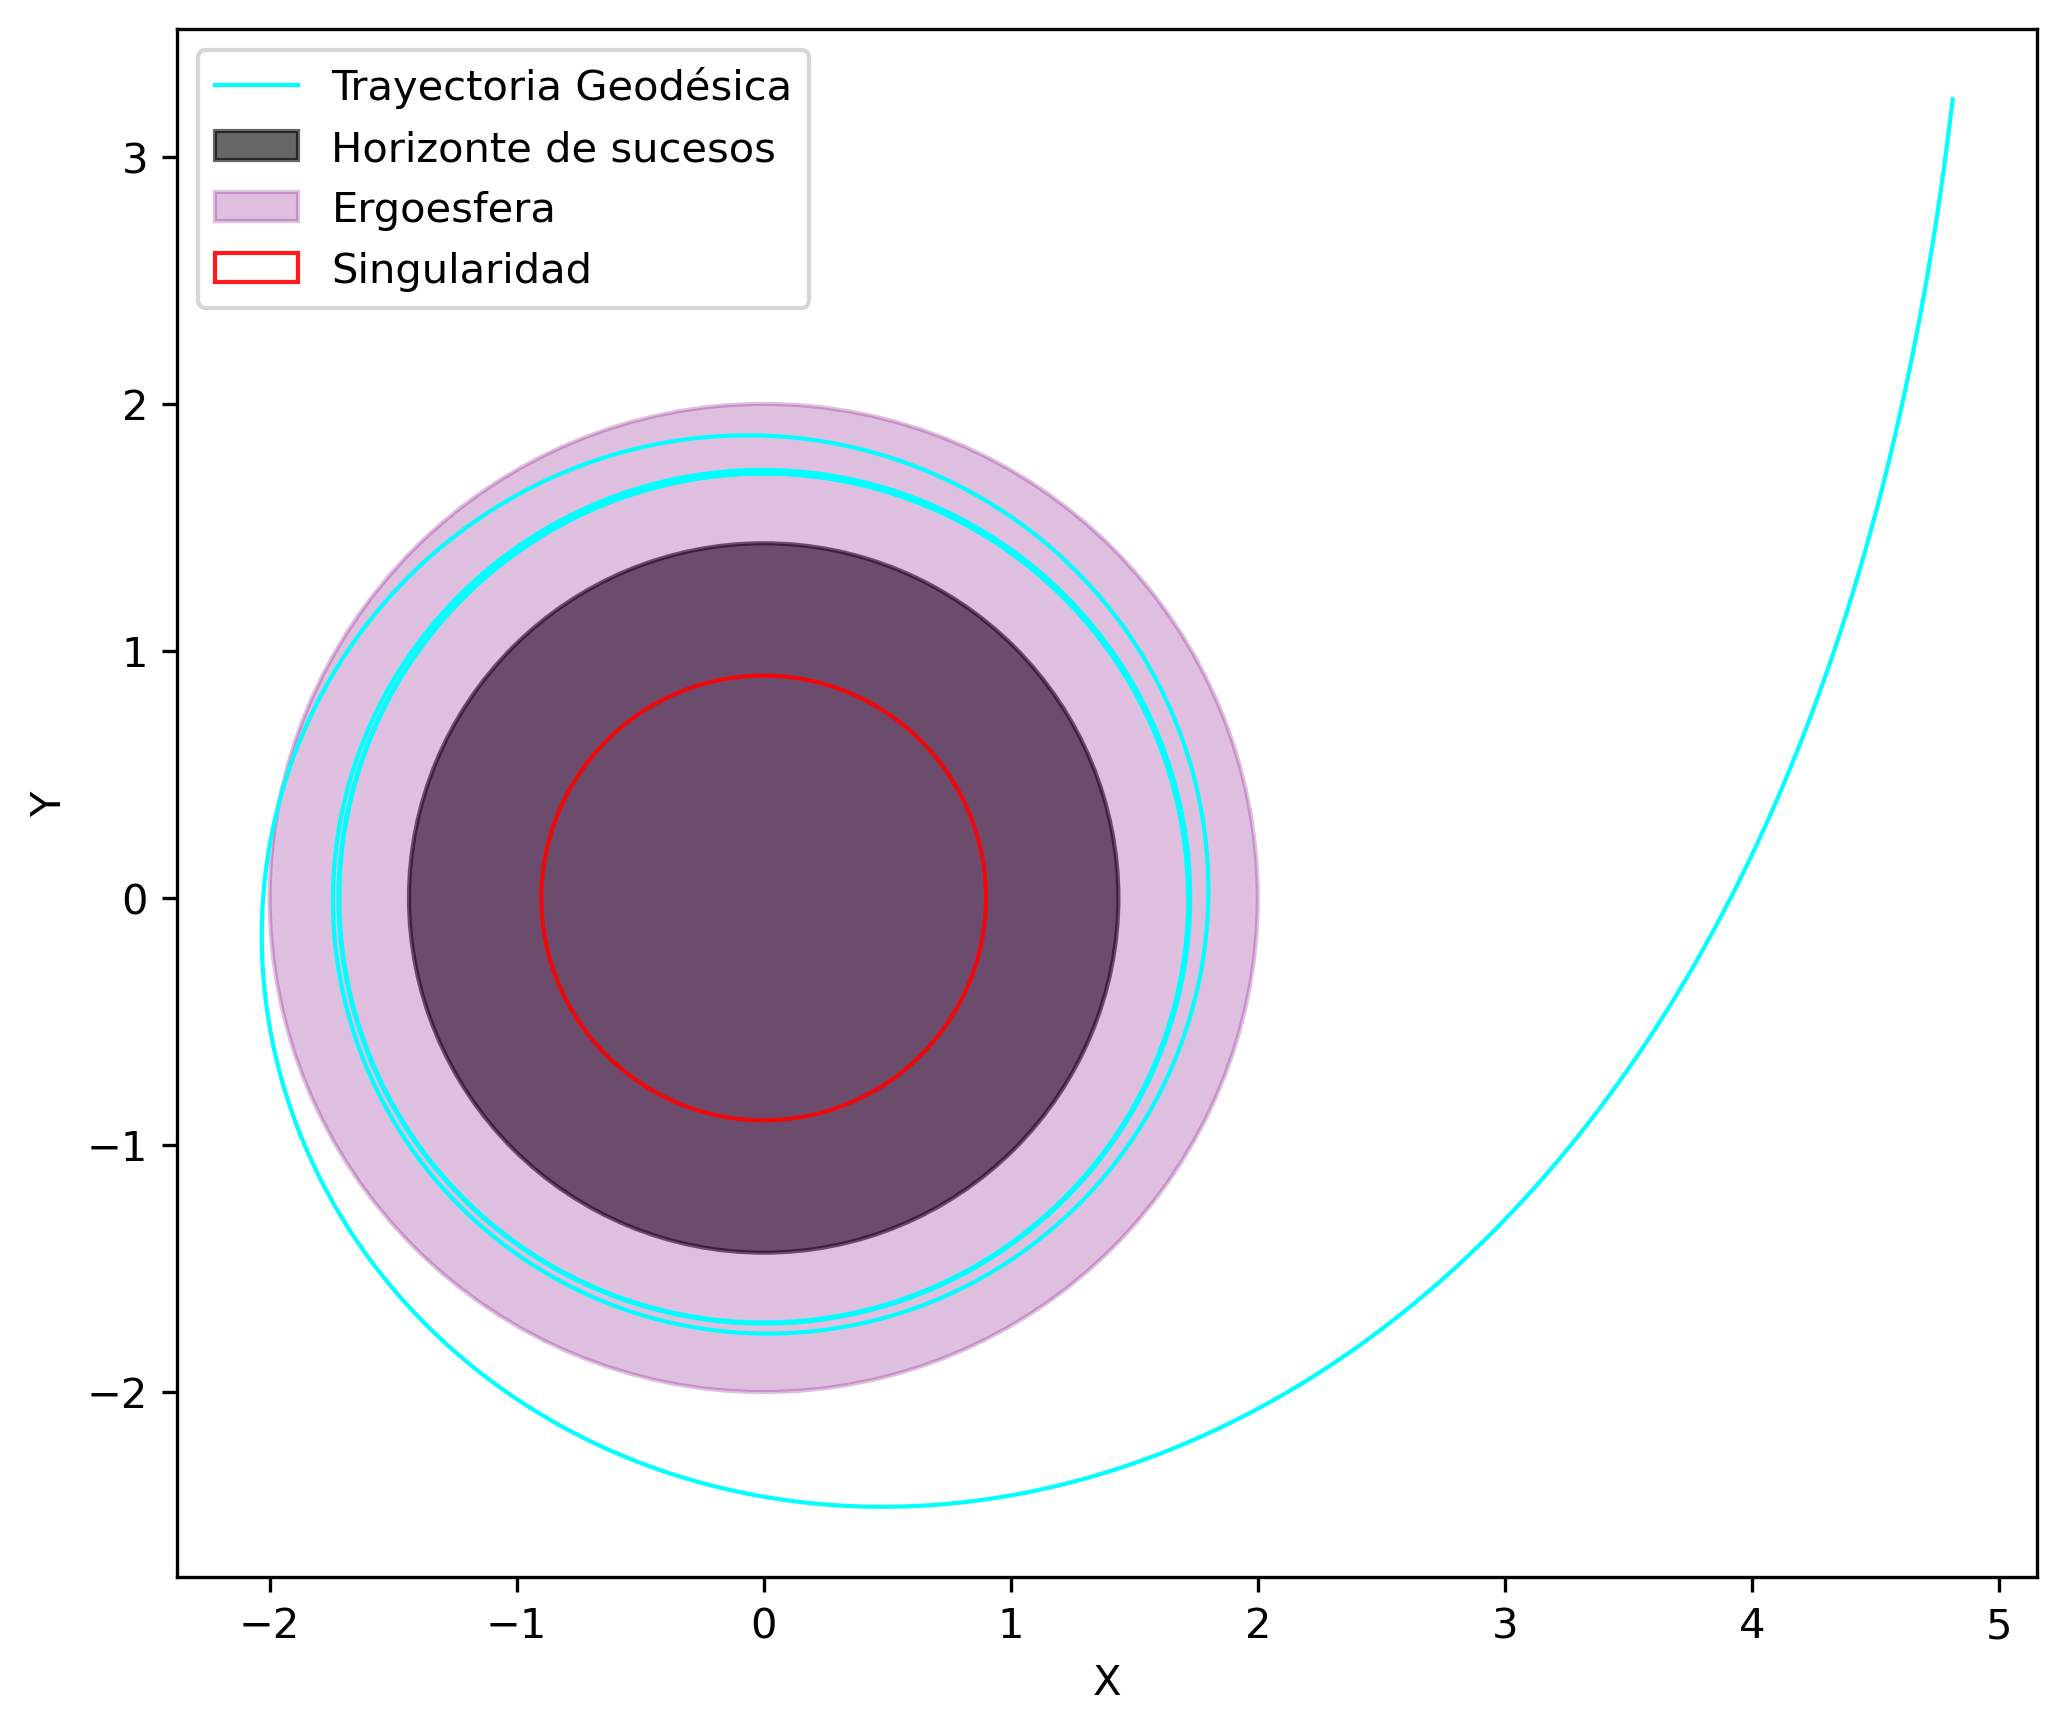
\includegraphics[width=\linewidth]{AgujerosNegros/kerr/geodesics_plots/geodesica_circular_r1,71_Q0_planoxy.png}
        \caption{Para $\mathrm{r}=1.7179$ y $\mathrm{Q}=0$, se uso $\mathrm{E}=1.021947$, $\mathrm{Lz}=2.701930$}
    \end{subfigure}
    \begin{subfigure}{0.4\textwidth}
        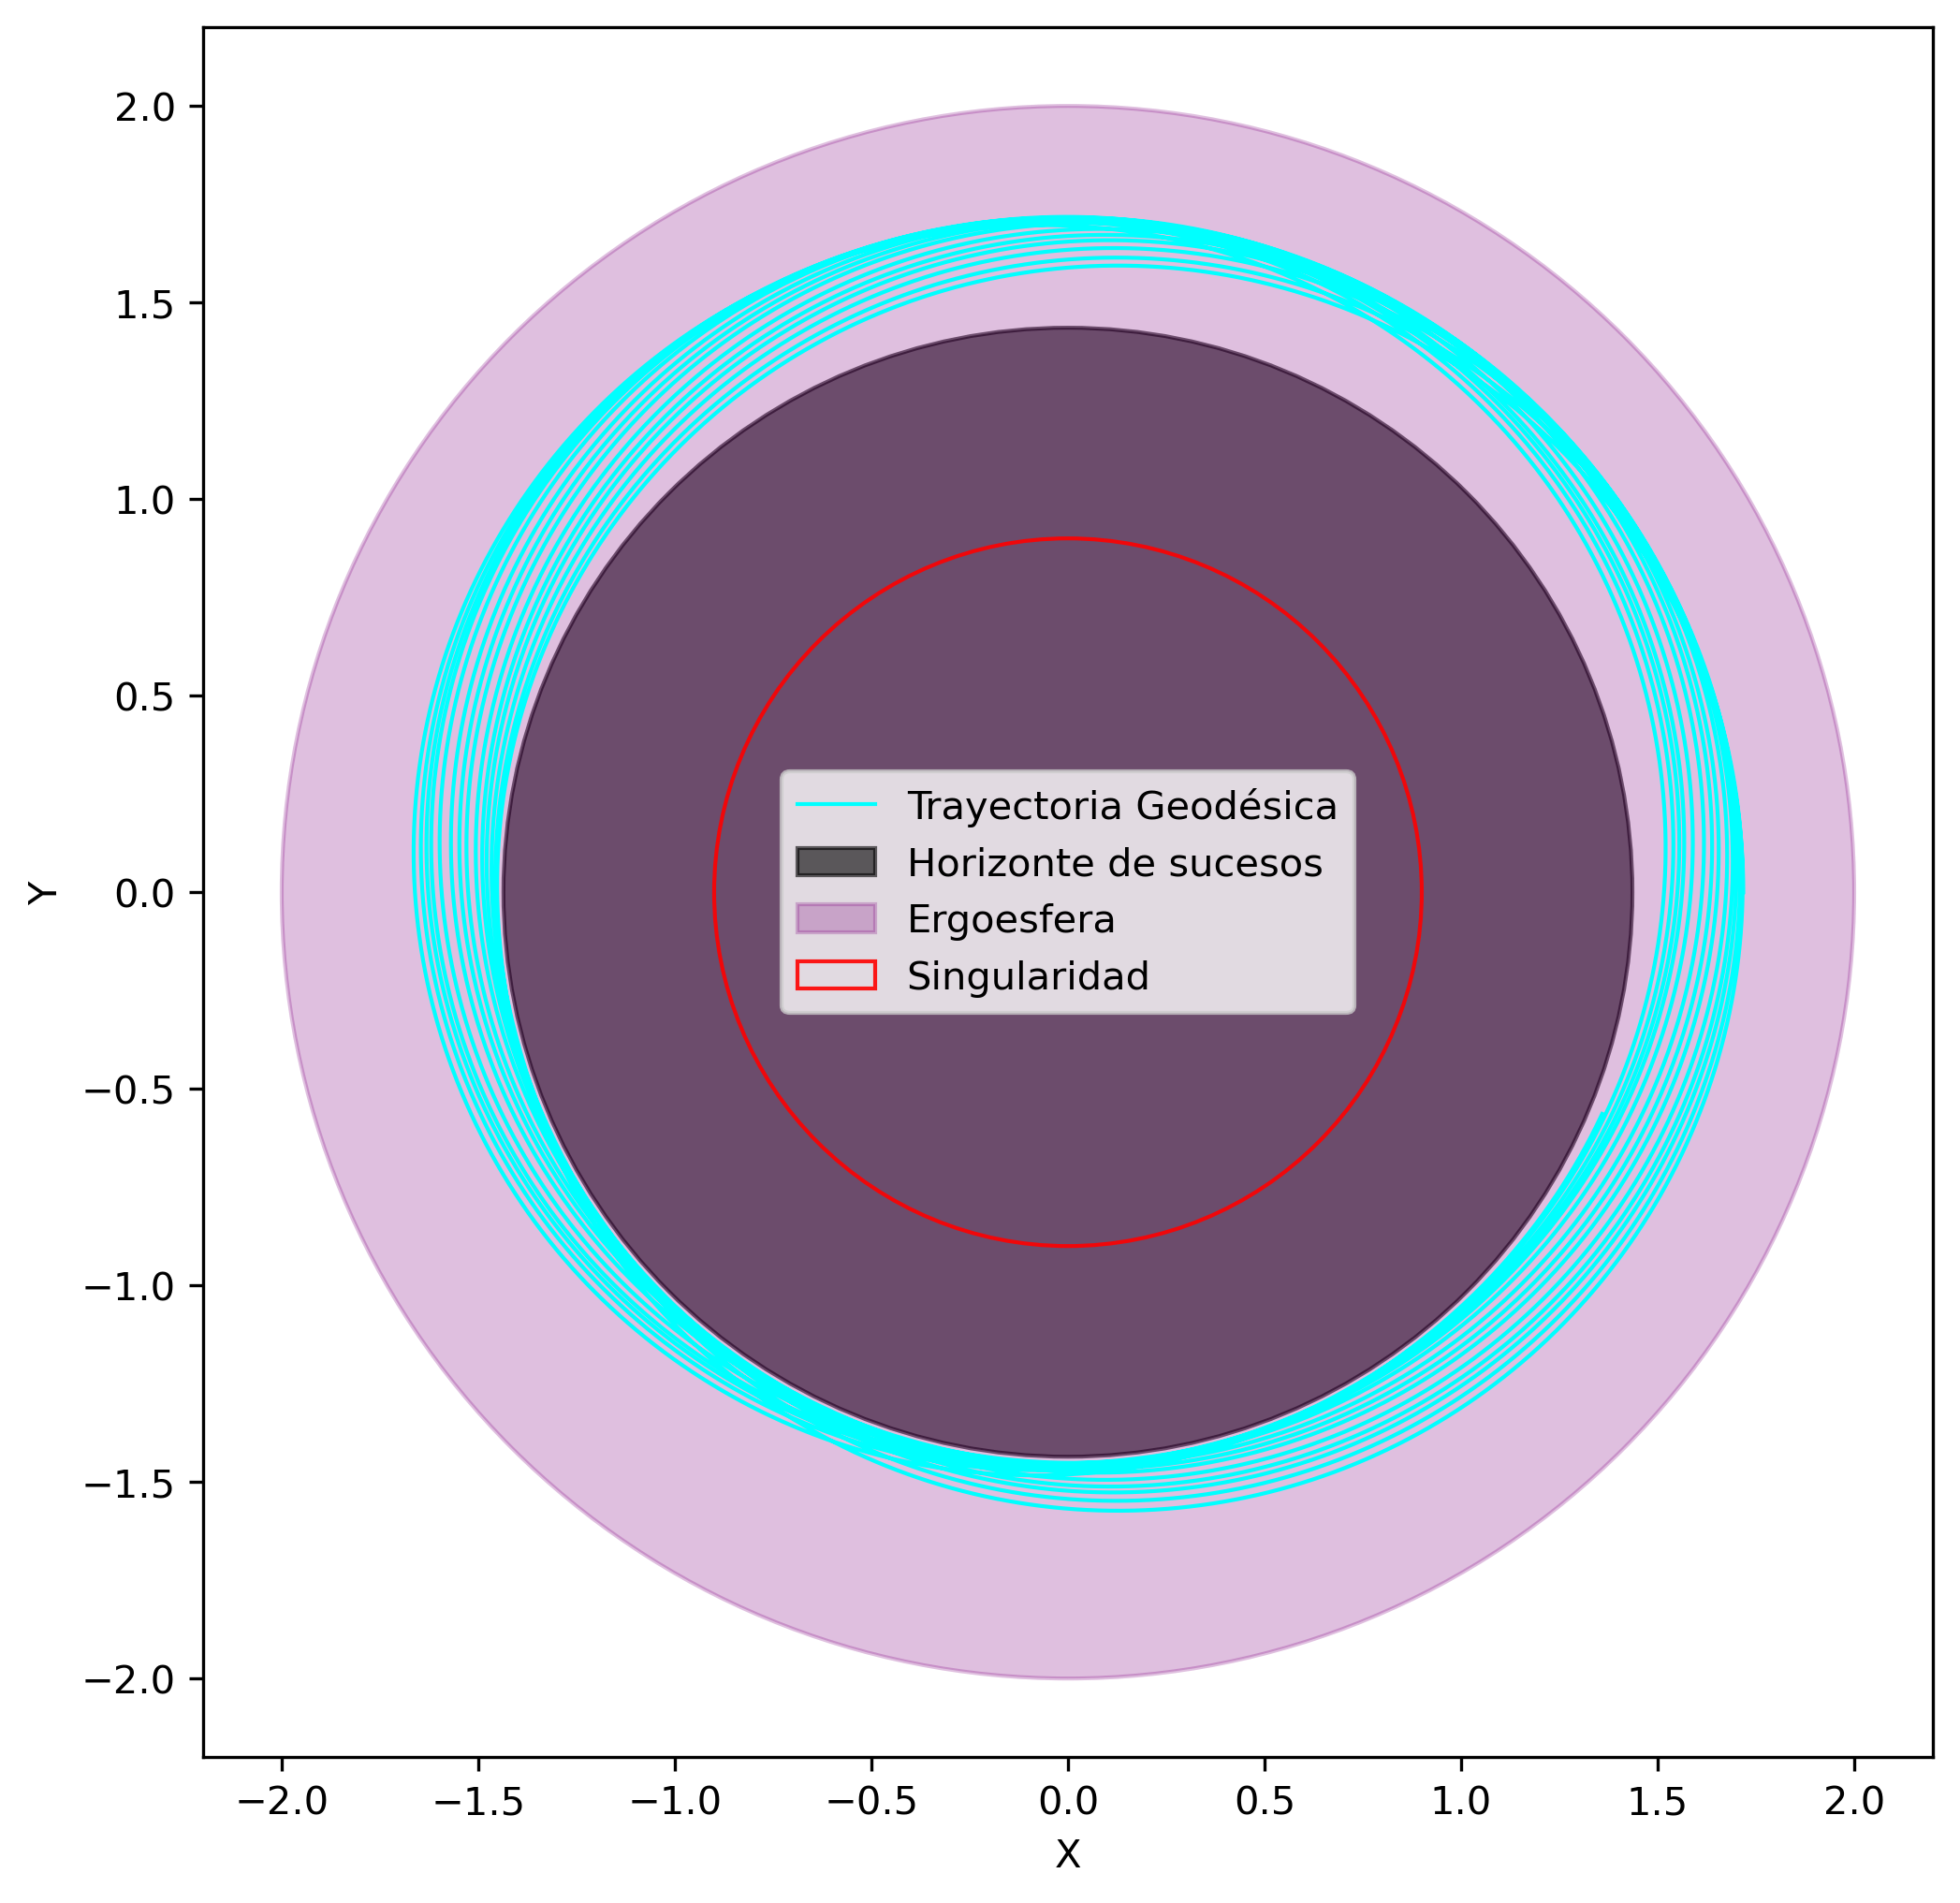
\includegraphics[width=\linewidth]{AgujerosNegros/kerr/geodesics_plots/geodesica_circular_r1,71_Q5_planoxy.png}
        \caption{Para $\mathrm{r}=1.7179$ y $\mathrm{Q}=5$, se uso $\mathrm{E}=1.418163$, $\mathrm{Lz}=3.607711$}
    \end{subfigure}
    \begin{subfigure}{0.4\textwidth}
        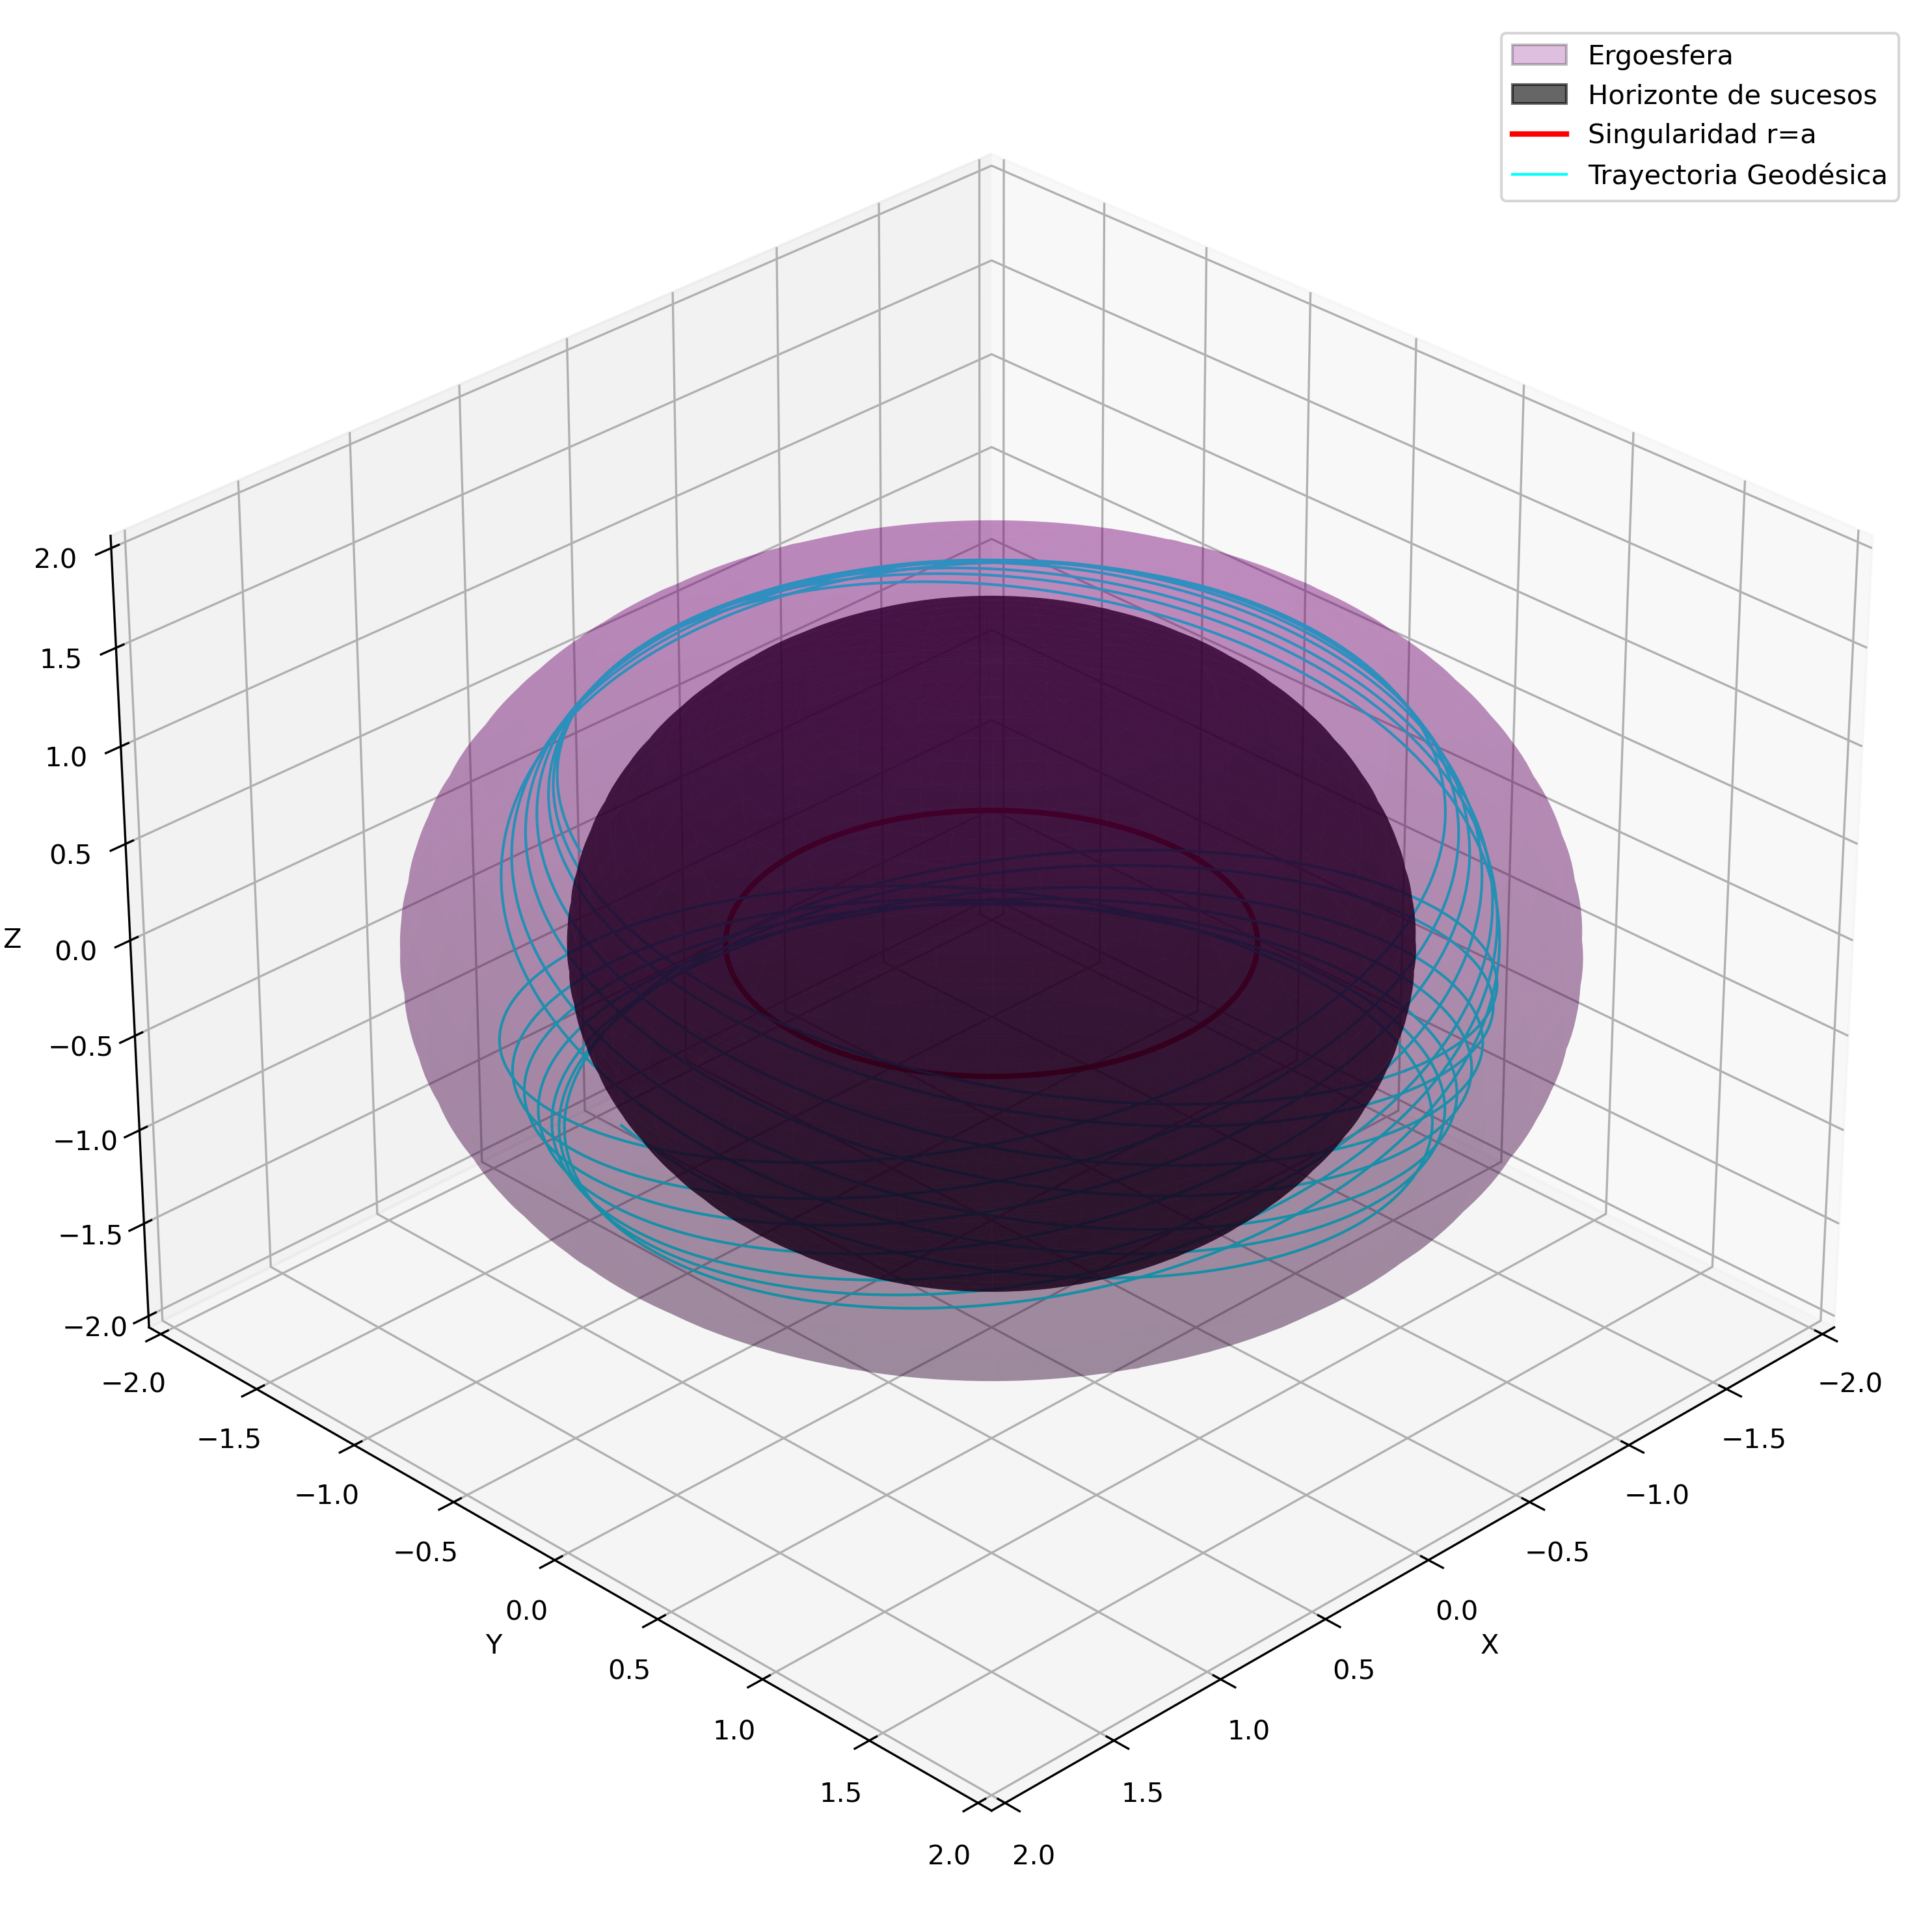
\includegraphics[width=\linewidth]{AgujerosNegros/kerr/geodesics_plots/geodesica_circular_r1,71_Q5.png}
        \caption{Misma órbita que la anterior pero vista en 3D.}
    \end{subfigure}

    \begin{subfigure}{0.4\textwidth}
        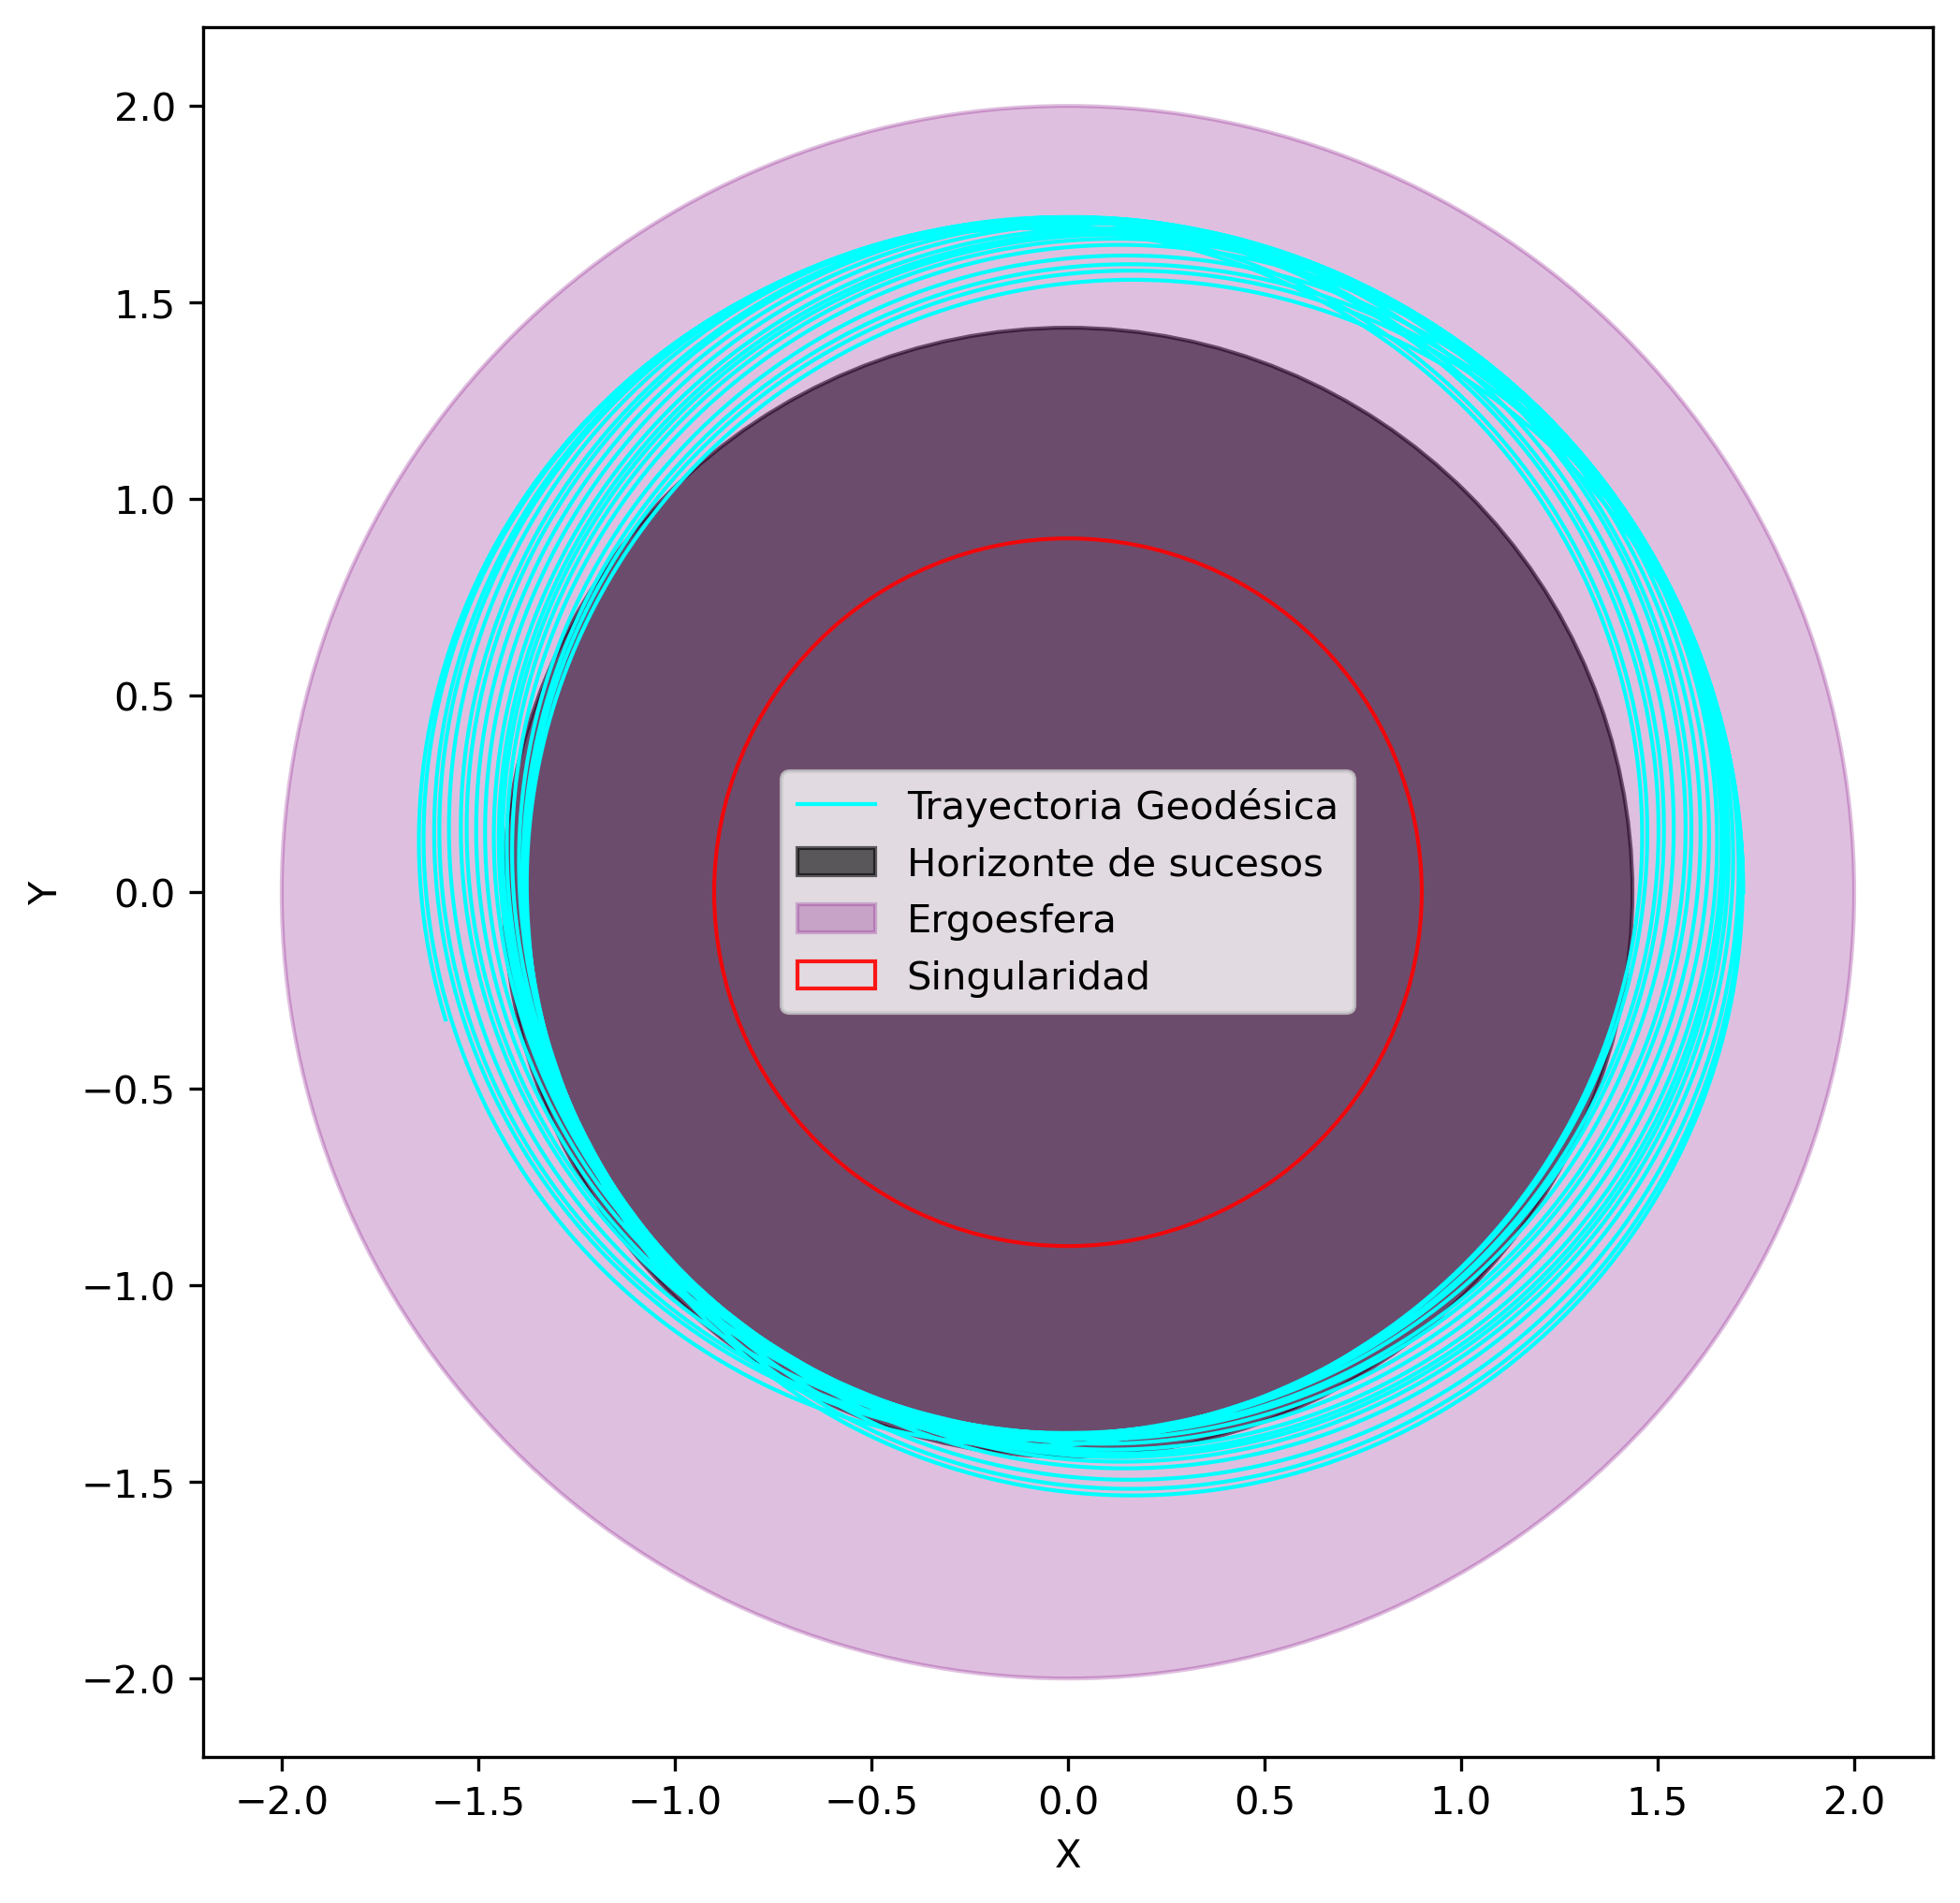
\includegraphics[width=\linewidth]{AgujerosNegros/kerr/geodesics_plots/geodesica_circular_r1,71_Q10_planoxy.png}
        \caption{Para $\mathrm{r}=1.7179$ y $\mathrm{Q}=10$, se uso $\mathrm{E}=1.730255$, $\mathrm{Lz}=4.345489$}
    \end{subfigure}
    \begin{subfigure}{0.5\textwidth}
        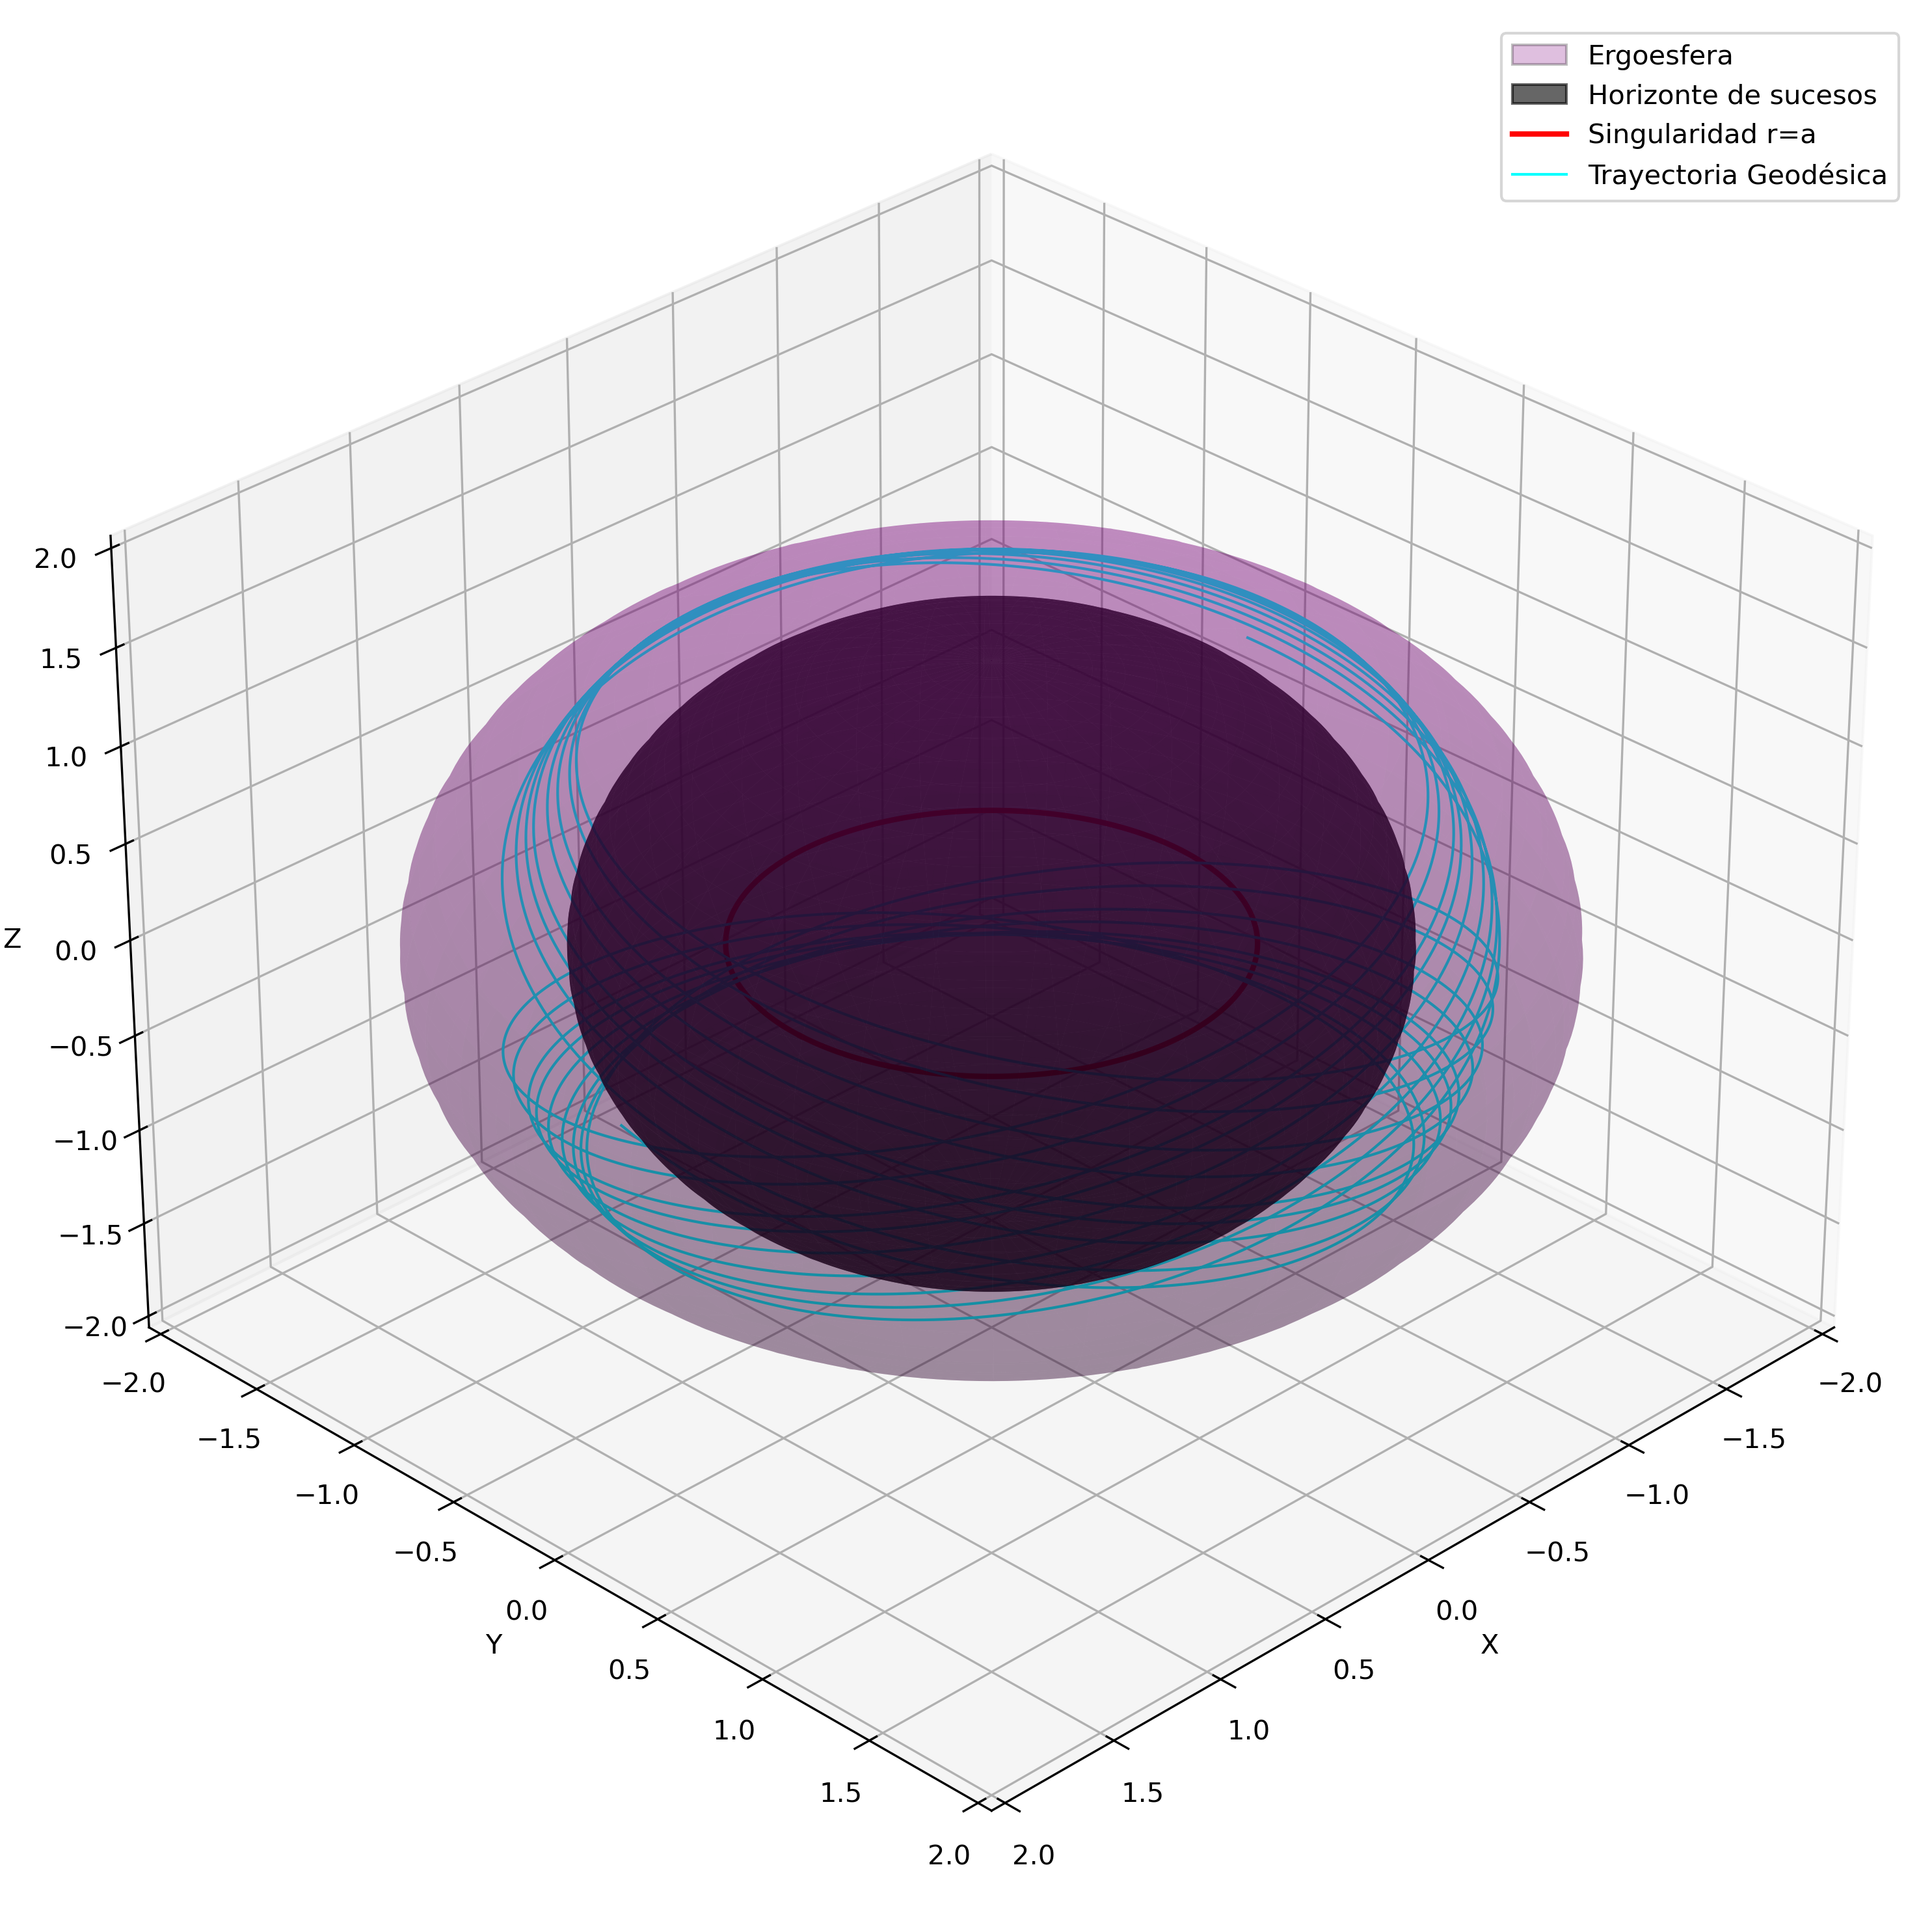
\includegraphics[width=\linewidth]{AgujerosNegros/kerr/geodesics_plots/geodesica_circular_r1,71_Q10.png}
        \caption{Misma órbita que la anterior pero vista en 3D.}
    \end{subfigure}
    \caption{Comparación de resultados obtenidos para diferentes condiciones.}
\end{figure}


\subsection{Geodesicas para fotones $\mu =0 $}
Las ecuacionies modificadas para Geodesicas
\begin{equation}
    g^{\mu \nu} \partial_\mu S \partial_\nu S= 0.
\end{equation}


Recordemos las funciones radiales y angulares que aparecen al separar la ecuación de Hamilton-Jacobi en el espacio-tiempo de Kerr para el caso nulo (\(\mu=0\)):

\begin{equation}
    R(r) = \big[(r^2+a^2)(E/c) - aL_z\big]^2 - \Delta \left[ (L_z - a(E/c))^2 + Q \right],
\end{equation}

\begin{equation}
    \Theta(\theta) = Q - \left( \frac{L_z^2}{\sin^2\theta} - a^2(E/c)^2 \right)\cos^2\theta.
\end{equation}
En ambas expresiones es posible factorizar la energía \(E\). Para \(R(r)\):

\begin{align}
    R(r) & = \left( (E/c) \left[ (r^2+a^2) - a\frac{L_z}{ (E/c) } \right]\right)^2
    - \Delta\left( \left(\frac{L_z}{(E/c)}-a\right)^2 + \frac{Q}{(E/c)^2} \right) (E/c)^2, \\
         & = (E/c)^2 \Bigg\{ \left[ (r^2+a^2) - a\frac{L_z}{(E/c)} \right]^2
    - \Delta\left( \left(\frac{L_z}{(E/c)}-a\right)^2 + \frac{Q}{(E/c)^2} \right) \Bigg\}.
\end{align}
De forma análoga, para la parte angular:

\begin{align}
    \Theta(\theta) & = Q - \left( \frac{L_z^2}{\sin^2\theta} - a^2 (E/c) ^2 \right)\cos^2\theta, \\
                   & = (E/c)^2 \Bigg[ \frac{Q}{(E/c)^2}
        - \left( \frac{(c L_z/E)^2}{\sin^2\theta} - a^2 \right)\cos^2\theta \Bigg].
\end{align}
En ambos casos aparece un factor común \((E/c)^2\).
Las ecuaciones de movimiento en tiempo de Mino \(\gamma\) son:

\begin{equation}
    \frac{dr}{d\gamma} = \pm \sqrt{R(r)}, \qquad
    \frac{d\theta}{d\gamma} = \pm \sqrt{\Theta(\theta)}.
\end{equation}
Dado que tanto \(R(r)\) como \(\Theta(\theta)\) contienen un factor global \((E/c)^2\),
podemos escribir

\begin{equation}
    \frac{dr}{d\gamma} = \pm (E/c) \sqrt{\tilde{R}(r)}, \qquad
    \frac{d\theta}{d\gamma} = \pm (E/c) \sqrt{\tilde{\Theta}(\theta)},
\end{equation}
donde \(\tilde{R}(r)\) y \(\tilde{\Theta}(\theta)\) ya no dependen de \((E/c)\).

Definimos un nuevo parámetro afín

\begin{equation}
    \lambda = (E/c)\gamma,
\end{equation}

de modo que

\begin{equation}
    \frac{dr}{d\lambda} = \pm \sqrt{\tilde{R}(r)}, \qquad
    \frac{d\theta}{d\lambda} = \pm \sqrt{\tilde{\Theta}(\theta)}.
\end{equation}

La energía \(E\) de un fotón sólo escala la parametrización de la curva,
pero no cambia la forma de la trayectoria en el espacio-tiempo.

En términos físicos, esto refleja el hecho de que todos los fotones, independientemente  de su frecuencia o energía, siguen la misma geodésica en un campo gravitatorio:
su destino está determinado únicamente por la dirección inicial y no por la magnitud de su energía.


Otra manera habitual de mostrar la independencia de la energía en las geodésicas nulas es mediante la introducción de los llamados \emph{parámetros de impacto}, definidos como

\begin{equation}
    \xi \equiv \frac{L_z}{(E/c)}, \qquad \eta \equiv \frac{Q}{(E/c)^2}.
\end{equation}

Estos parámetros son adimensionales y encapsulan las cantidades conservadas en cocientes
que eliminan la dependencia en la escala de energía \((E/c)\).


Los parámetros de impacto \(\xi=L_z/(E/c)\) y \(\eta=Q/(E/c)^2\) son simplemente
una notación conveniente para encapsular la información en cantidades adimensionales.

Sustituyendo estas definiciones en las expresiones de los potenciales radial y angular:

\begin{align}
    R(r)           & =  (r^2+a^2 - a\xi)^2 - \Delta\big((\xi - a)^2 + \eta \big) ,           \\
    \Theta(\theta) & =  \eta - \left( \frac{\xi^2}{\sin^2\theta} - a^2 \right)\cos^2\theta .
\end{align}

Para mayor simplicidad podemos imponer $E/c = 1$, de modo que las constantes de movimiento quedan como $L_z = \xi$ y $Q = \eta$.
\subsubsection{Geodésicas nulas radiales}
En este caso $L_z = 0$ y $Q = 0$, y $E = 1$, supondremos una distancia inicial de $r_0 = 6m$.
\begin{figure}[H]
    \begin{small}
        \begin{center}
            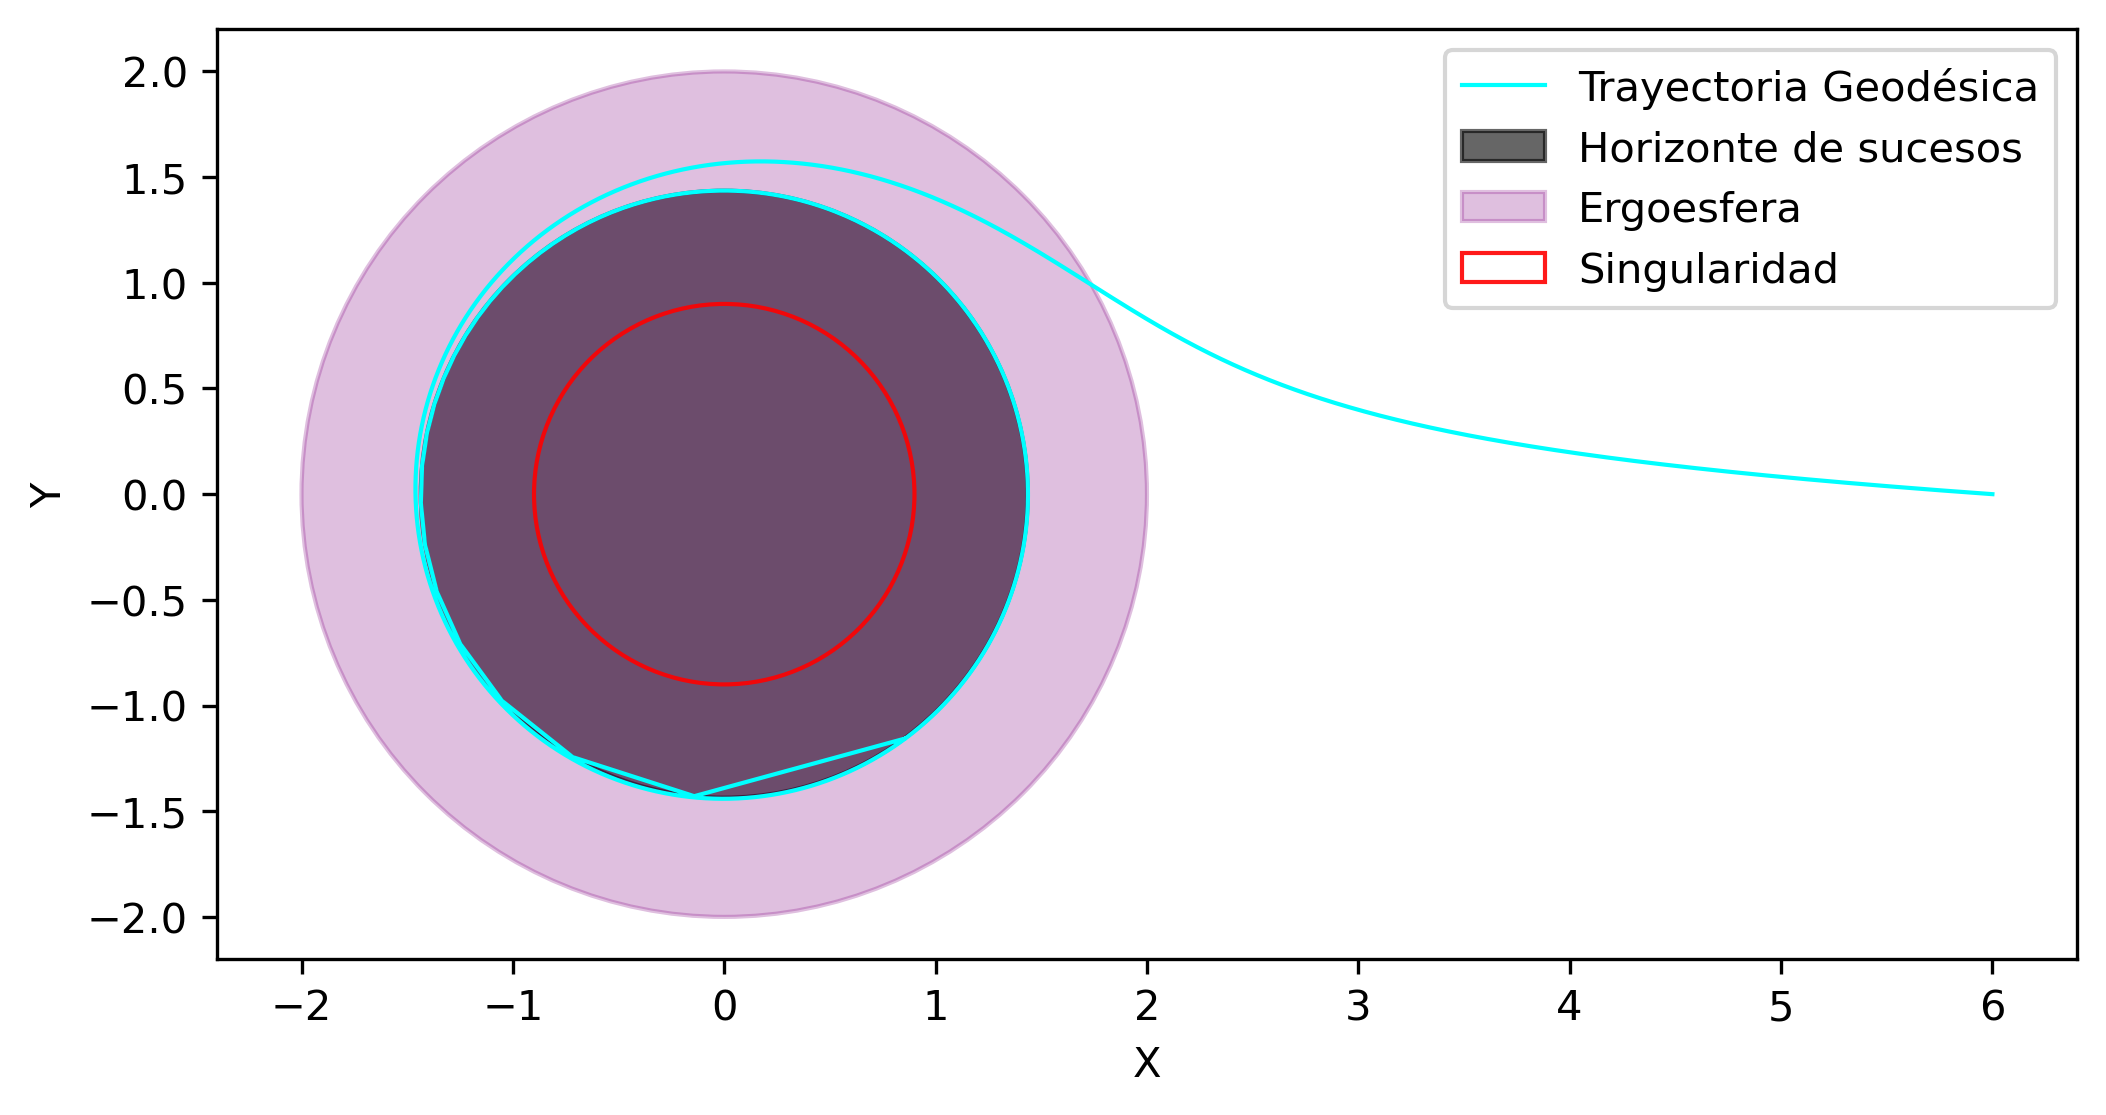
\includegraphics[width=0.95\textwidth]{AgujerosNegros/kerr/geodesics_plots/geodesica_foton_caida_planoxy.png}
        \end{center}
        \caption{Geodesica nula en caída libre en Kerr con $a = 0.9$, $m=1$ y $c=1$.}
    \end{small}
\end{figure}

\subsubsection{Geodésicas circulares para fotones}
Para este caso solo debemos de preocuparnos de los 2 parametros de impacto $\xi$ y $\eta$, y el radio de la órbita circular $r_c$.

El codigo para calcular las constantes en funcion de $r_c$ es practicamenrte el mismo que el del anexo \ref{chap:programa_orbitas_circulares_kerr} pero con las siguientes modificaciones:


\begin{lstlisting}[language=Python, caption={Cálculo numérico de las constantes para órbitas circulares de fotones en Kerr}, label={lst:kerr_circular_orbits_photons}]
    import sympy as sp

# --- Símbolos ---
r = sp.Symbol('r', real=True)
xi, eta = sp.symbols('xi eta', real=True)
a, m = sp.symbols('a m', real=True)

# Definiciones
Delta = r**2 - 2*m*r + a**2
R_expr = (r**2 + a**2 - a*xi)**2 - Delta * ((xi - a)**2 + eta)

# Condiciones para órbitas de fotones
eq1 = sp.Eq(R_expr, 0)
eq2 = sp.Eq(sp.diff(R_expr, r), 0)

# Parámetros del agujero negro
params = {a:0.9, m:1.0}

# Ejemplo: órbita de fotón en r=3M
r_val = 1.70
sol = sp.solve([eq1.subs({**params, r:r_val}),
                eq2.subs({**params, r:r_val})],
               [xi, eta], dict=True)

print(f"Soluciones para r={r_val}:")
for s in sol:
    xi_val = float(s[xi].evalf())
    eta_val = float(s[eta].evalf())
    print(f"xi = {xi_val:.6f}, eta = {eta_val:.6f}")
\end{lstlisting}

A continuacion se muestran las gráficas de las constantes de impacto $\xi$ y $\eta$ en función del radio $r_c$ para órbitas circulares de fotones.
\begin{figure}[H]
    \begin{subfigure}{0.5\textwidth}
        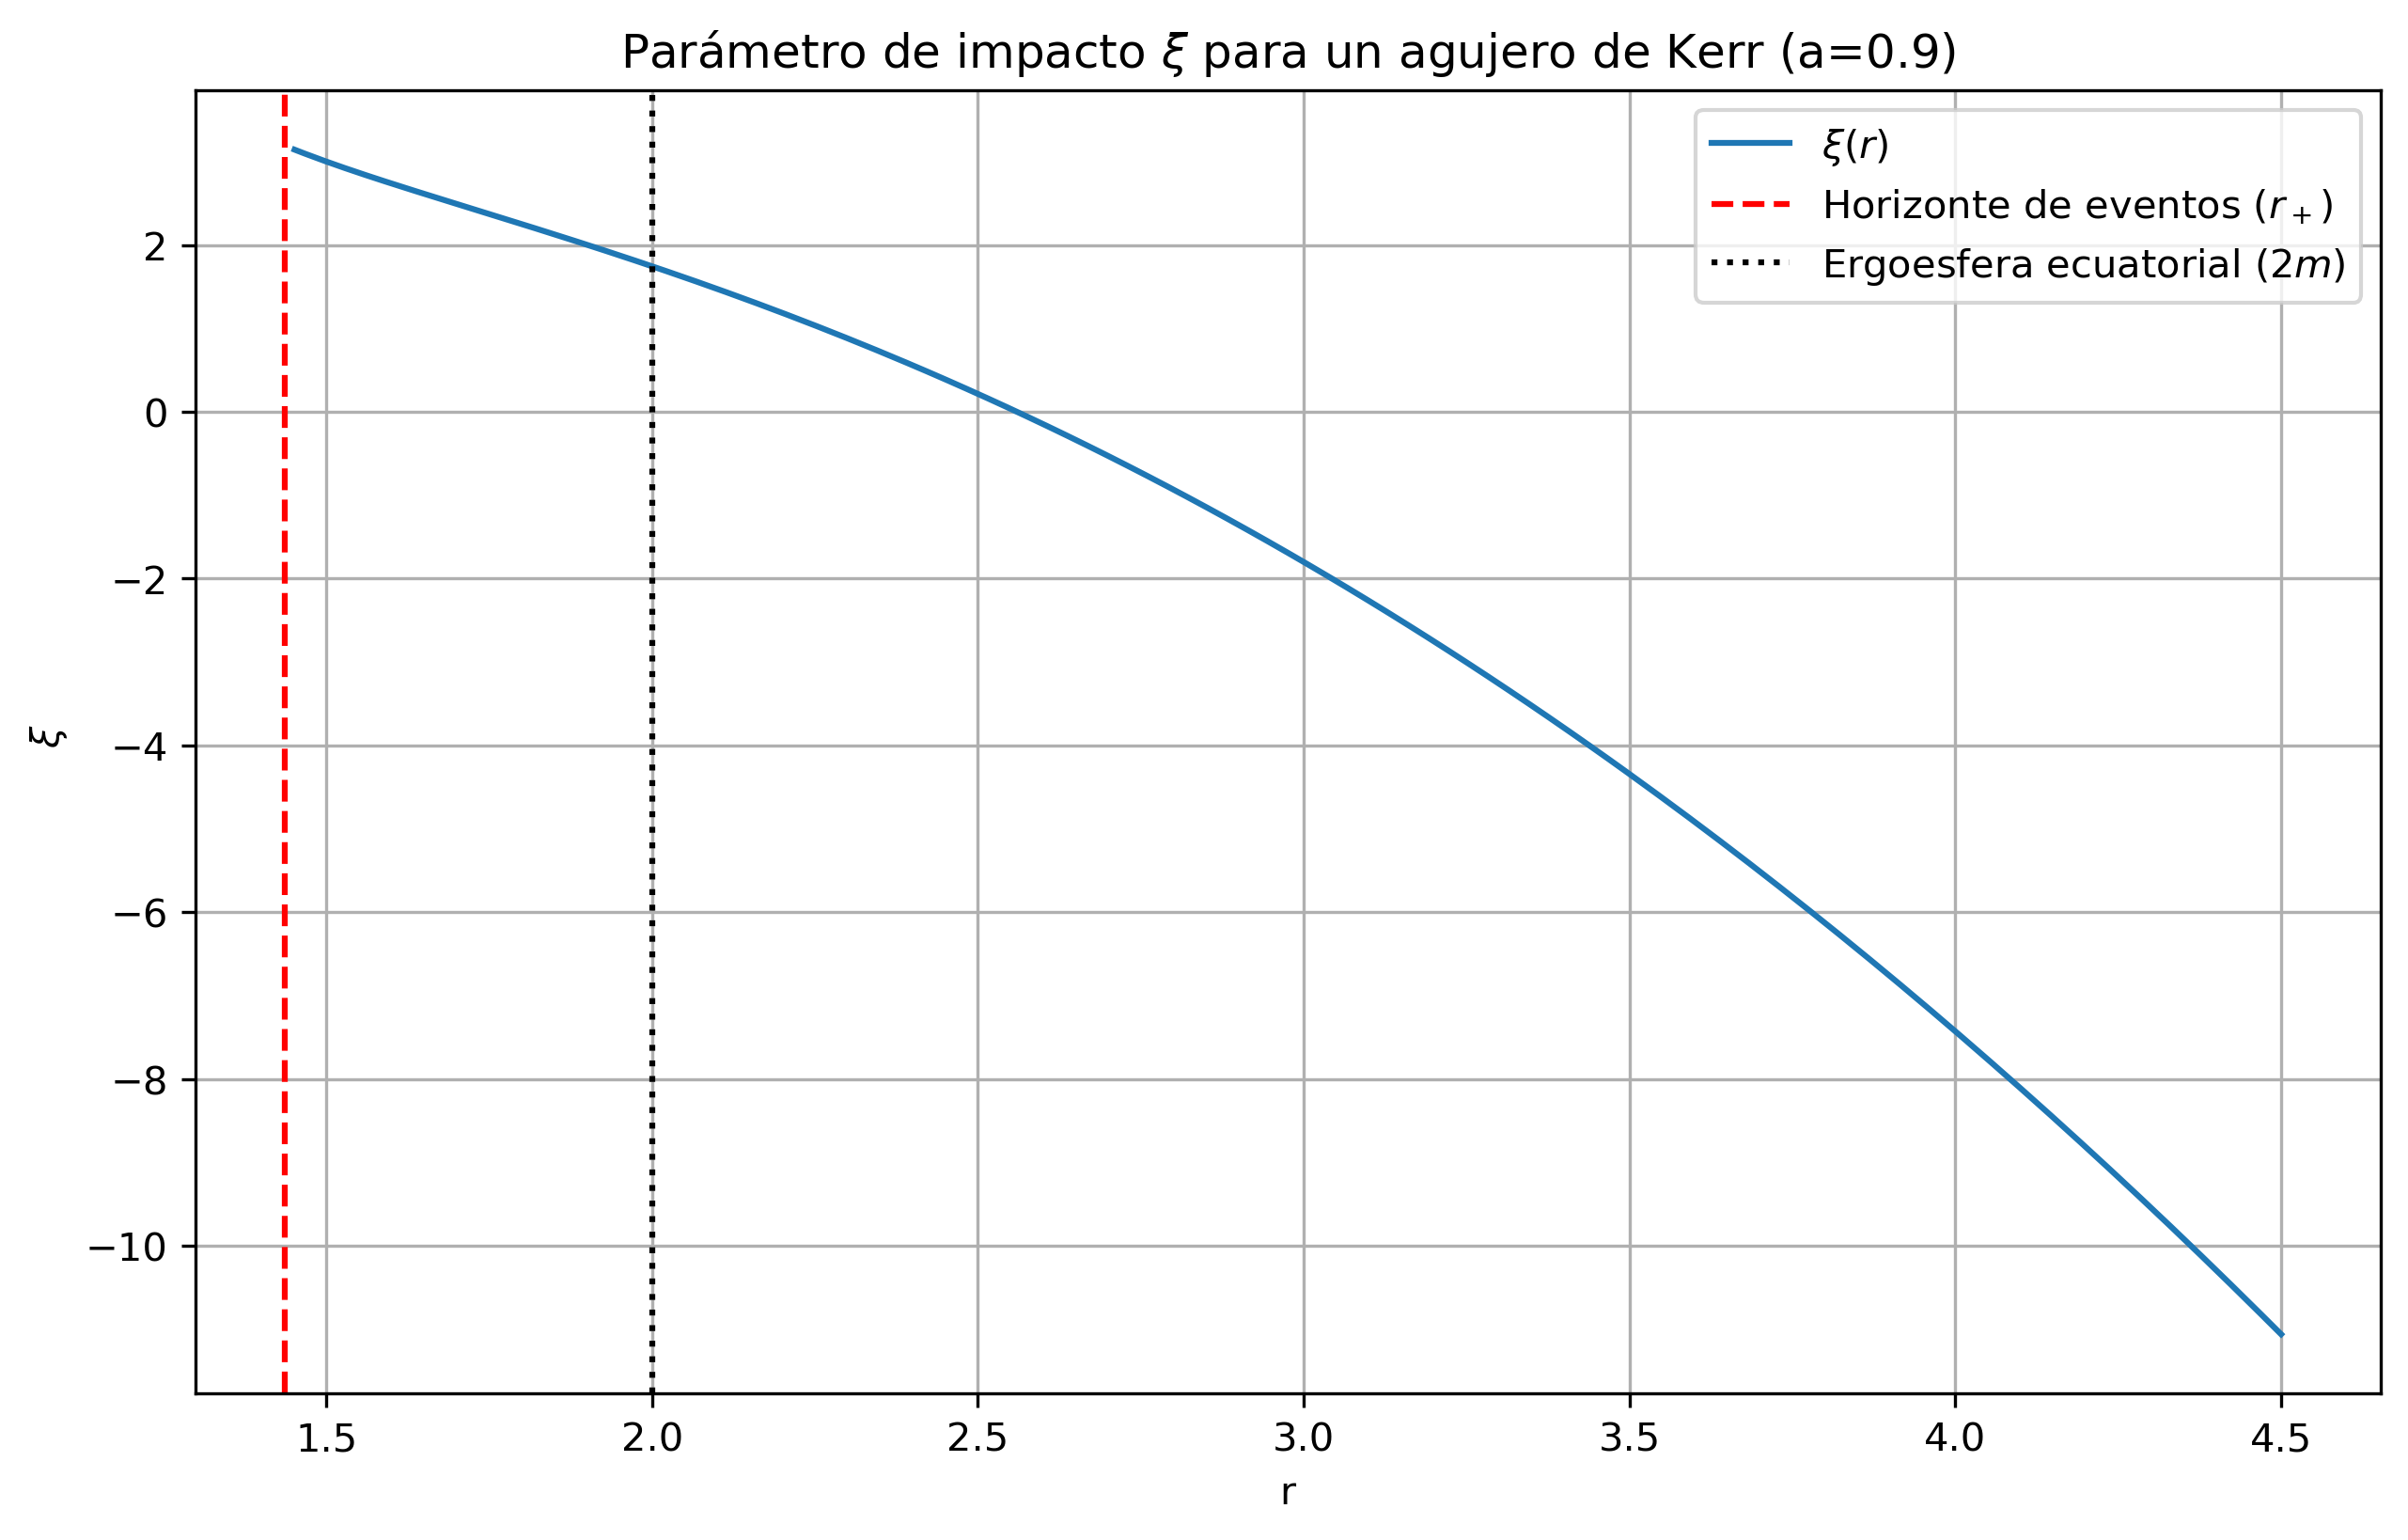
\includegraphics[width=0.9\linewidth, height=6cm]{AgujerosNegros/kerr/geodesics_plots/circular_xi_vs_r_kerr.png}
        \caption{Constante de impacto $\xi$ en función del radio $r$.}
    \end{subfigure}
    \begin{subfigure}{0.5\textwidth}
        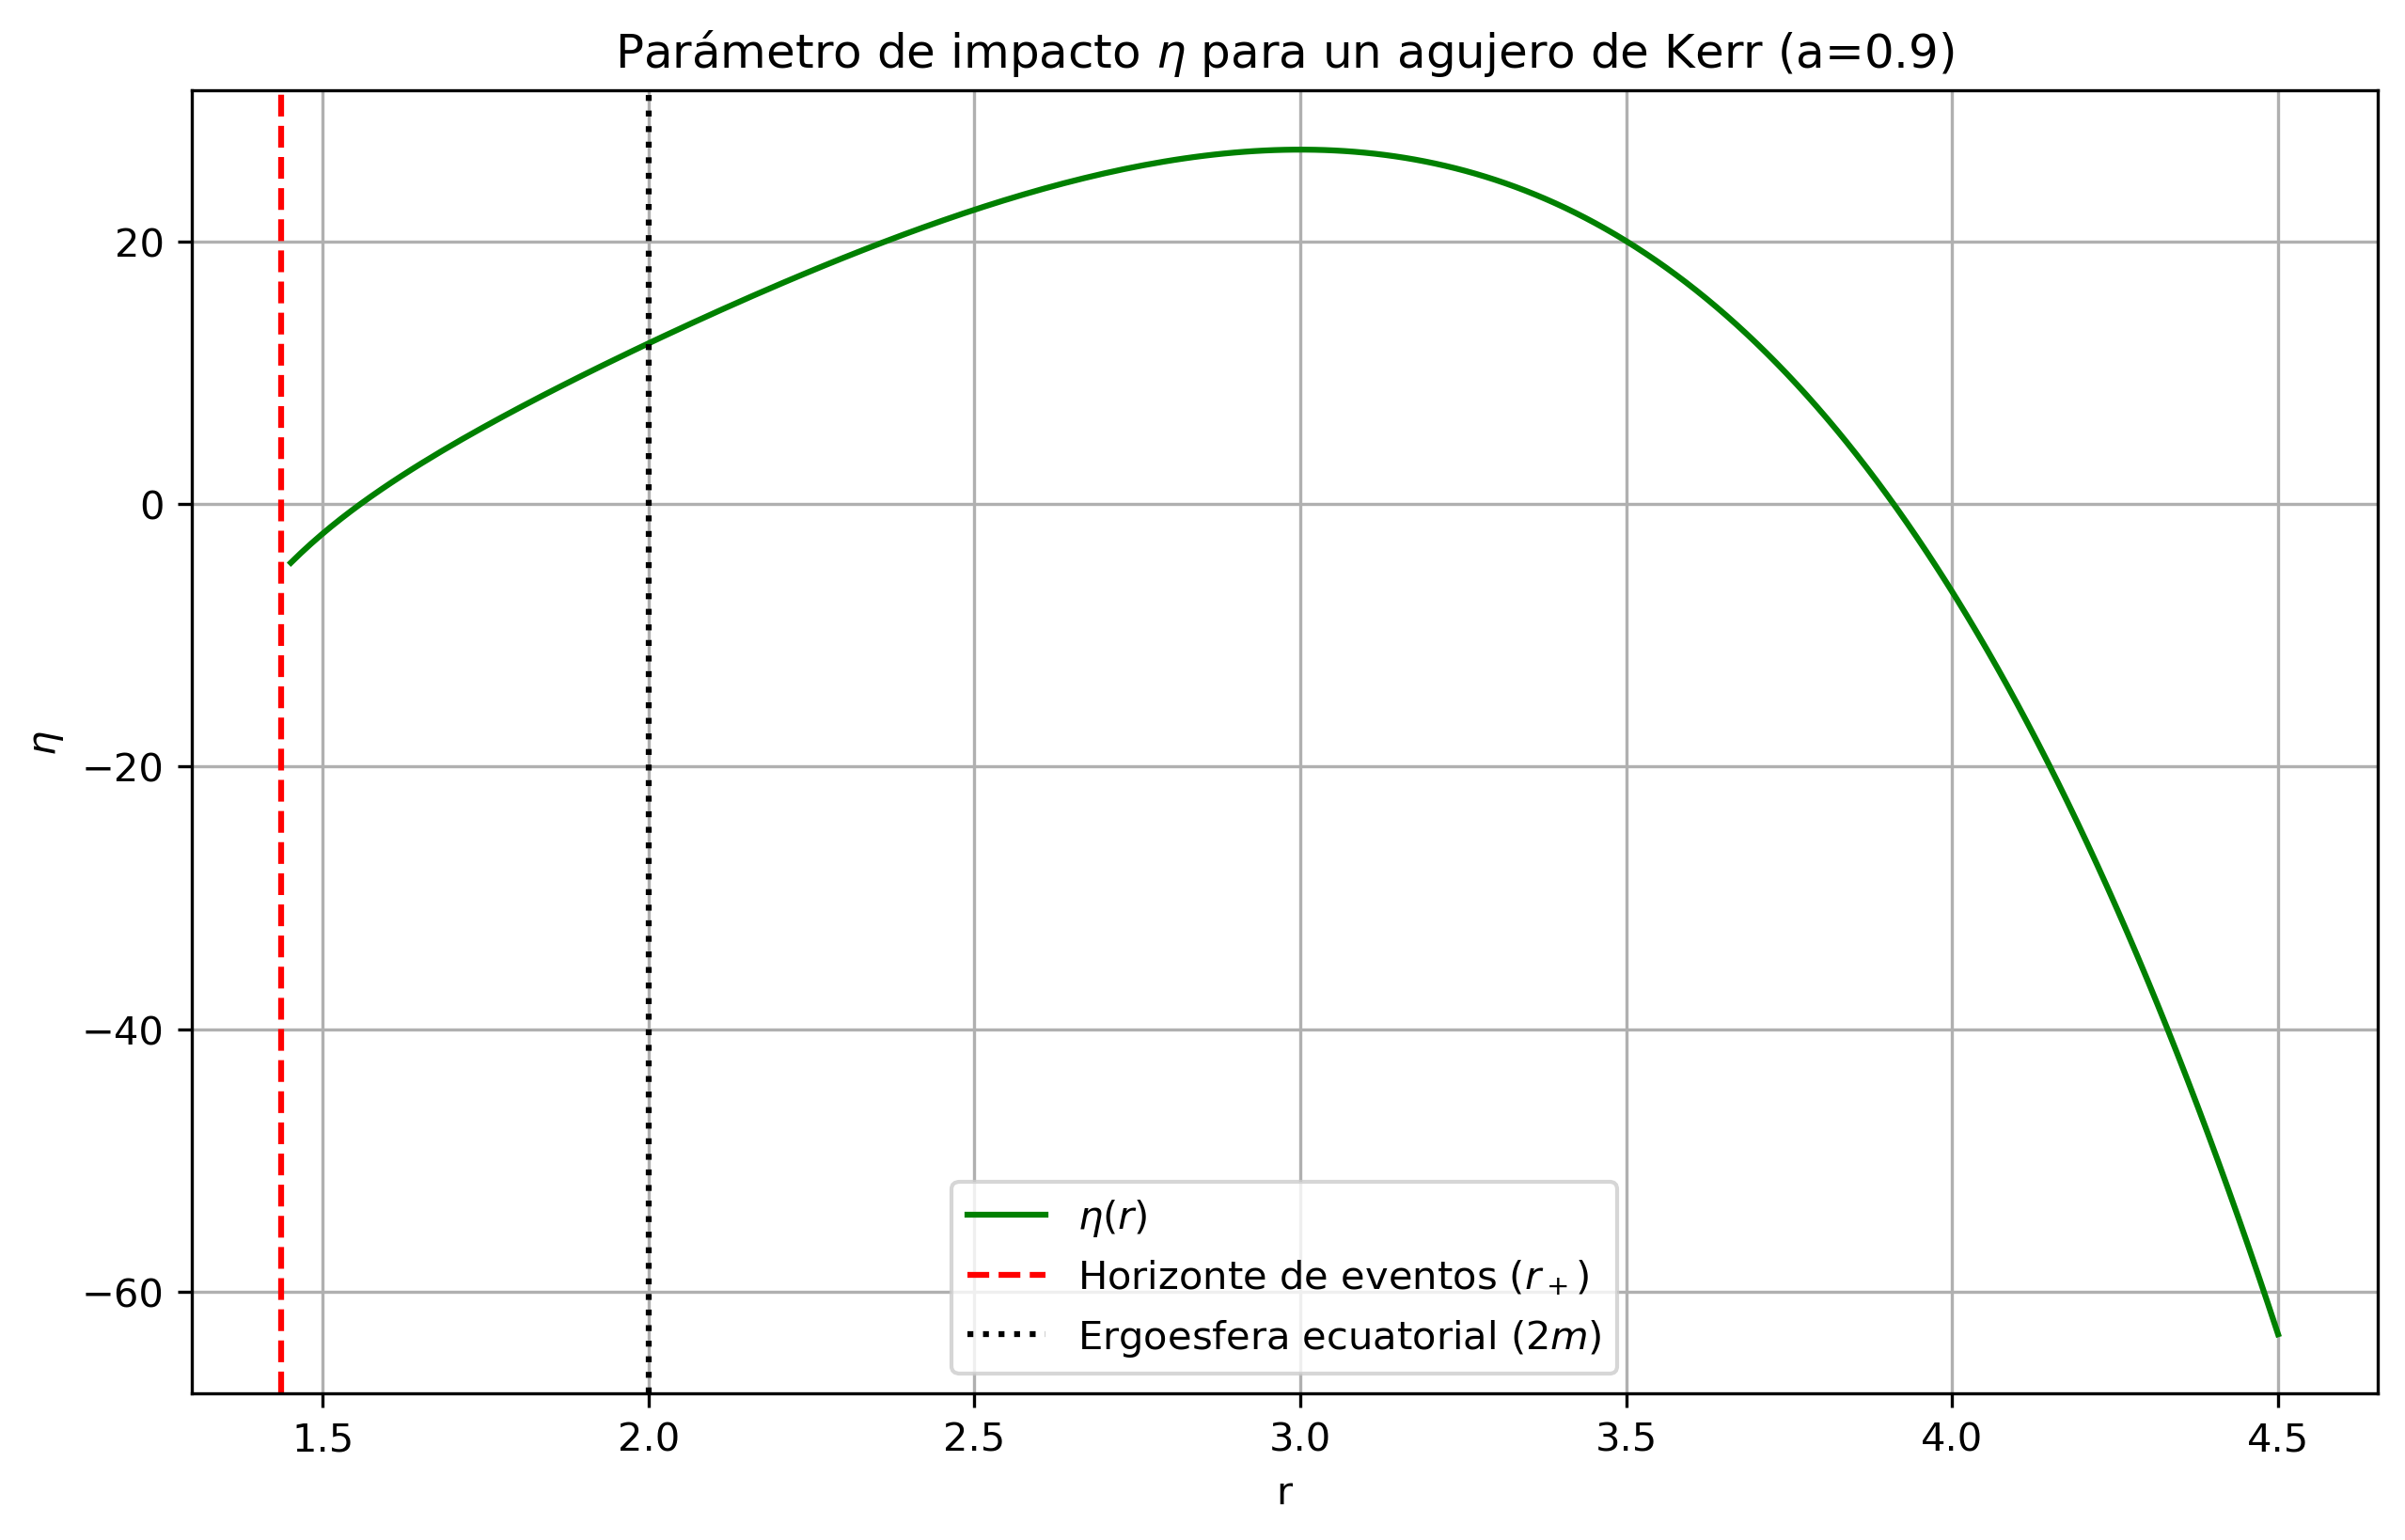
\includegraphics[width=0.9\linewidth, height=6cm]{AgujerosNegros/kerr/geodesics_plots/circular_eta_vs_r_kerr.png}
        \caption{Constante de impacto $\eta$ en función del radio $r$.}
    \end{subfigure}
    \caption{Gráficas de las constantes $\xi$ y $\eta$ en función del radio $r$.}
\end{figure}
Por ejemplo, para una órbita circular en $r_c = 3m$ se obtienen las siguientes soluciones:
\begin{equation}
    \begin{array}{l}
        \text{Soluciones para } r=3:              \\
        \xi = 10.900000,\quad \eta = -100.000000, \\
        \xi = -1.800000,\quad \eta = 27.000000.
    \end{array}
\end{equation}
Dado que la solución con $\eta < 0$ no es físicamente admisible, se selecciona la segunda opción.

\begin{figure}[H]
    \begin{small}
        \begin{center}
            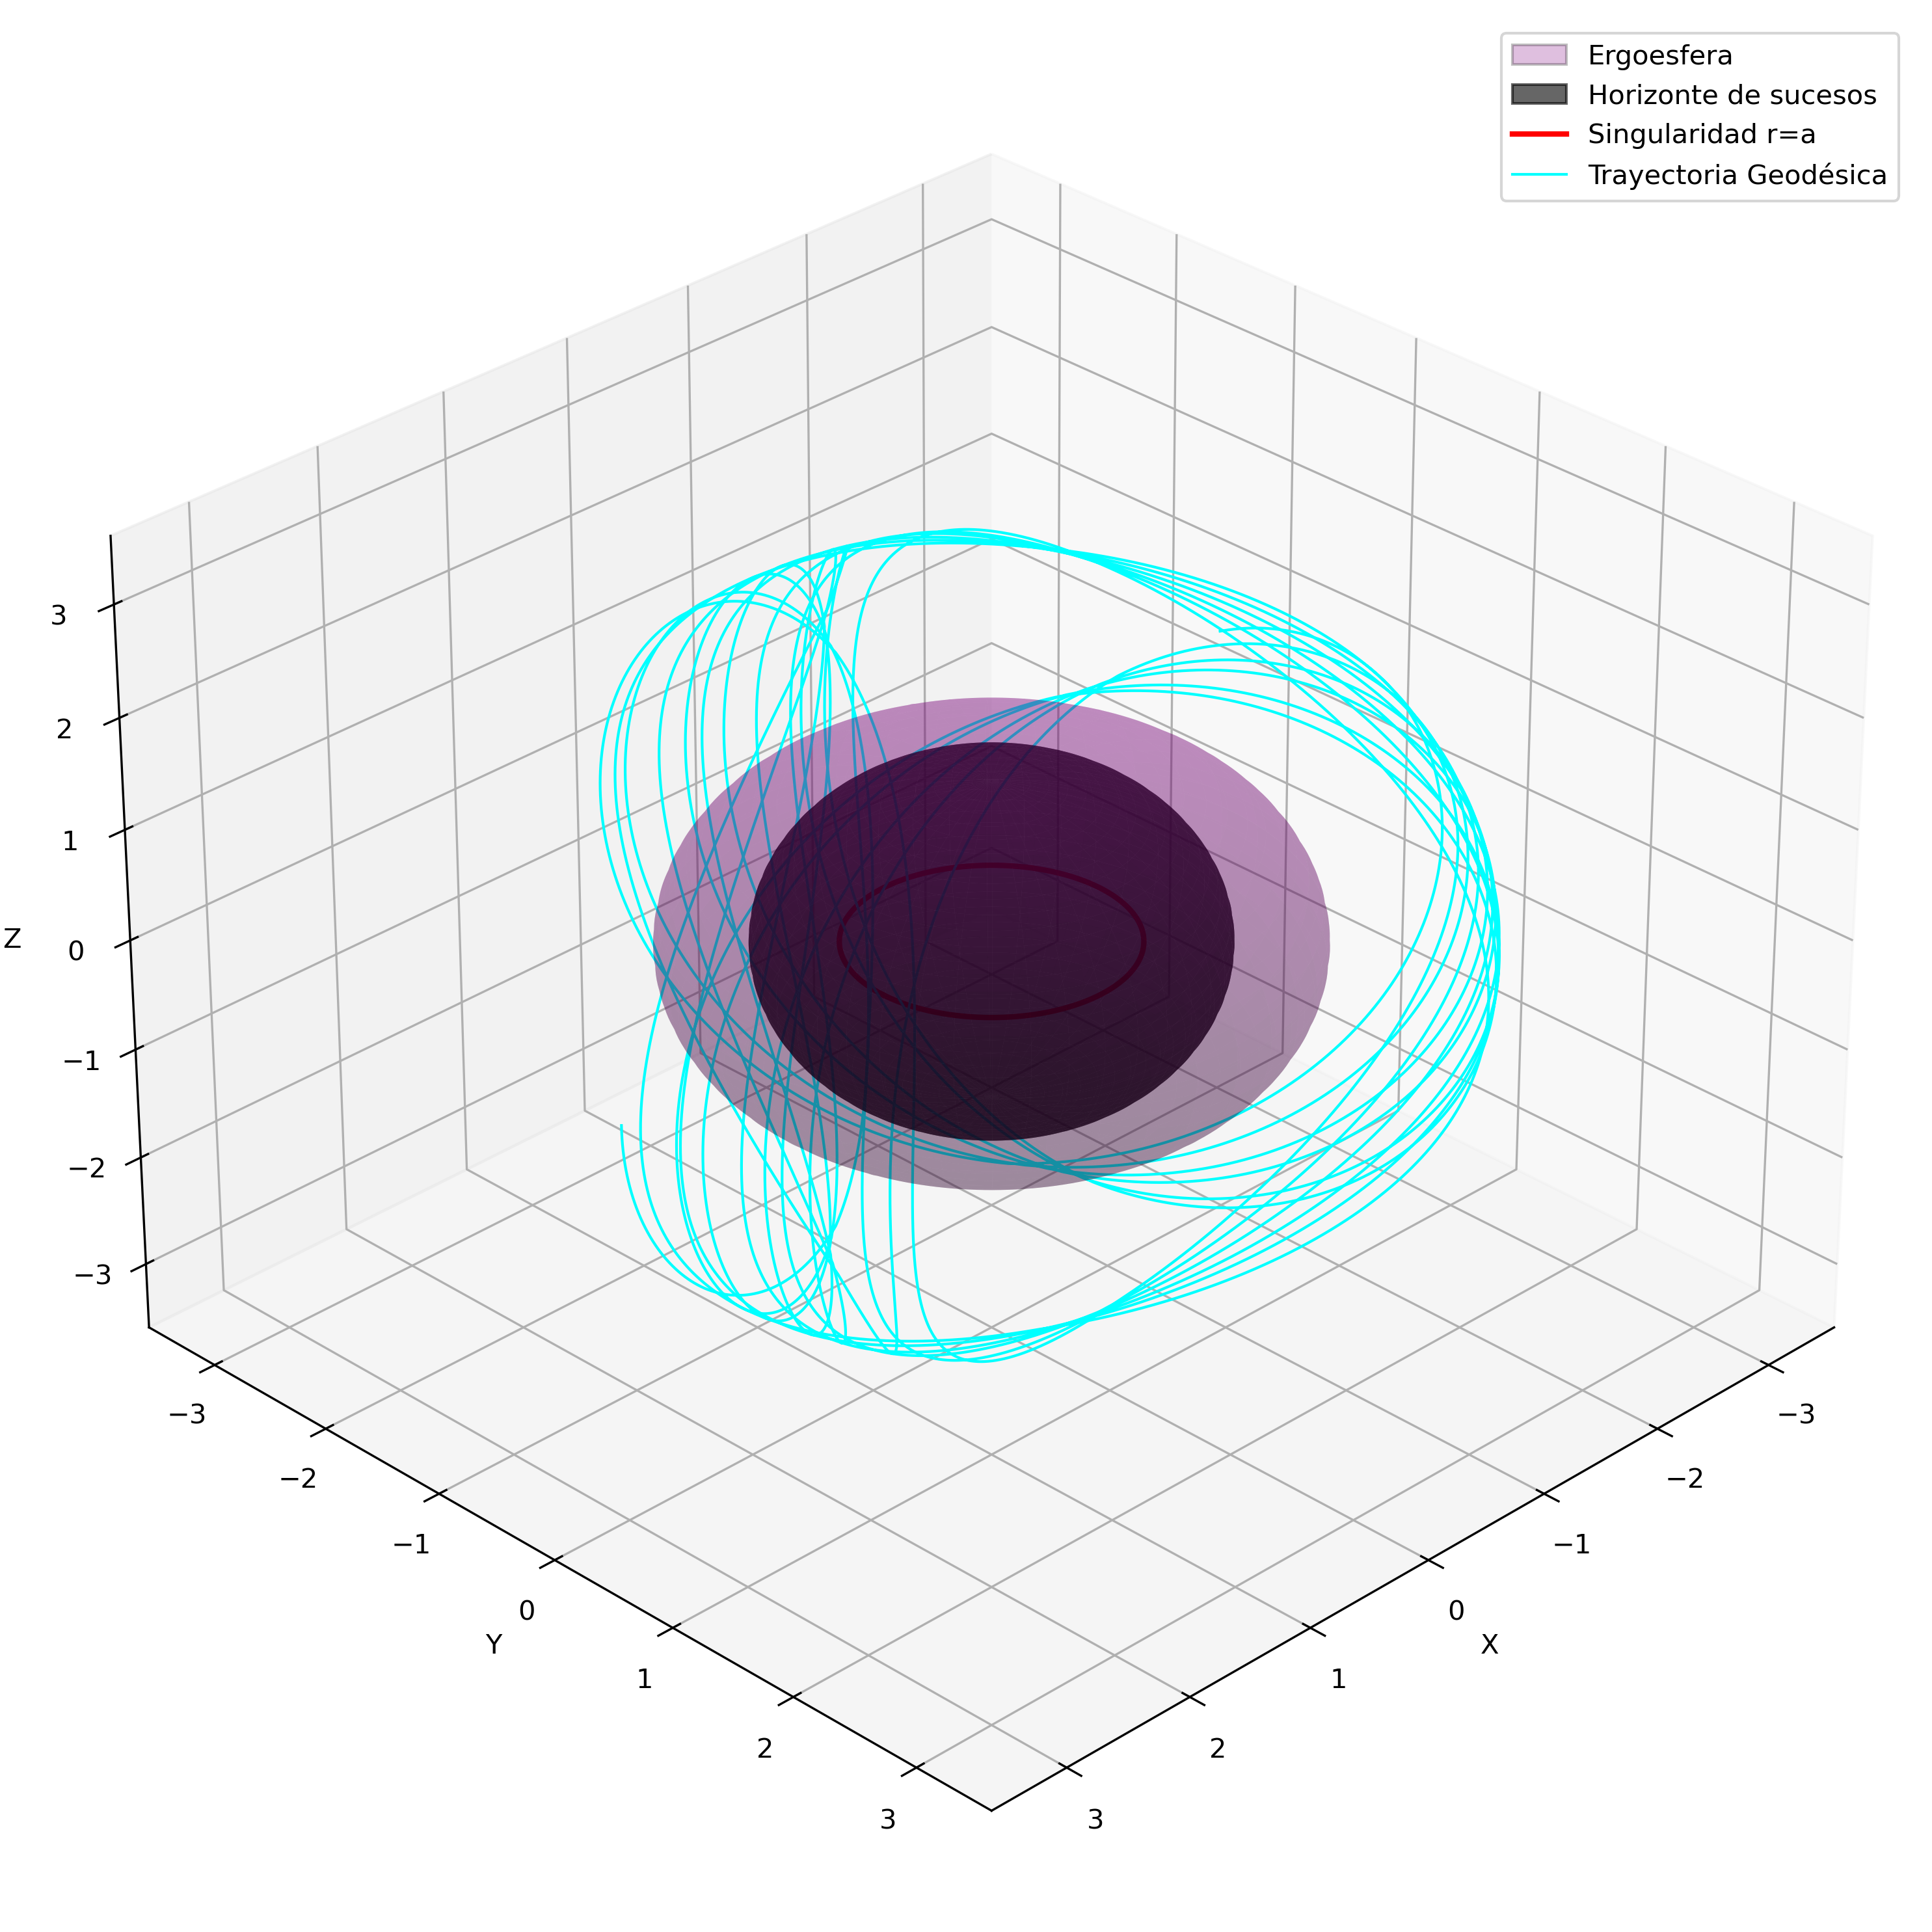
\includegraphics[width=0.95\textwidth]{AgujerosNegros/kerr/geodesics_plots/geodesica_circular_foton_r3.png}
        \end{center}
        \caption{Geodésica circular de fotón en Kerr con $a = 0.9$, $m=1$ y $c=1$.}
        \label{fig:geodesica_circular_foton_r3}
    \end{small}
\end{figure}

De igual forma, para una órbita circular ubicada en la región intermedia entre el horizonte y la ergoesfera en el ecuador (es decir, para $r=1.7179$), se obtienen:
\begin{equation}
    \begin{array}{l}
        \text{Soluciones para } r=1.7179: \\
        \begin{array}{l}
            \xi = 4.179089,\quad \eta = -10.752427, \\
            \xi = 2.448824,\quad \eta = 5.053942.
        \end{array}
    \end{array}
\end{equation}
Nuevamente, al descartar la solución con $\eta < 0$, se opta por la segunda alternativa.

\begin{figure}[H]
    \begin{small}
        \begin{center}
            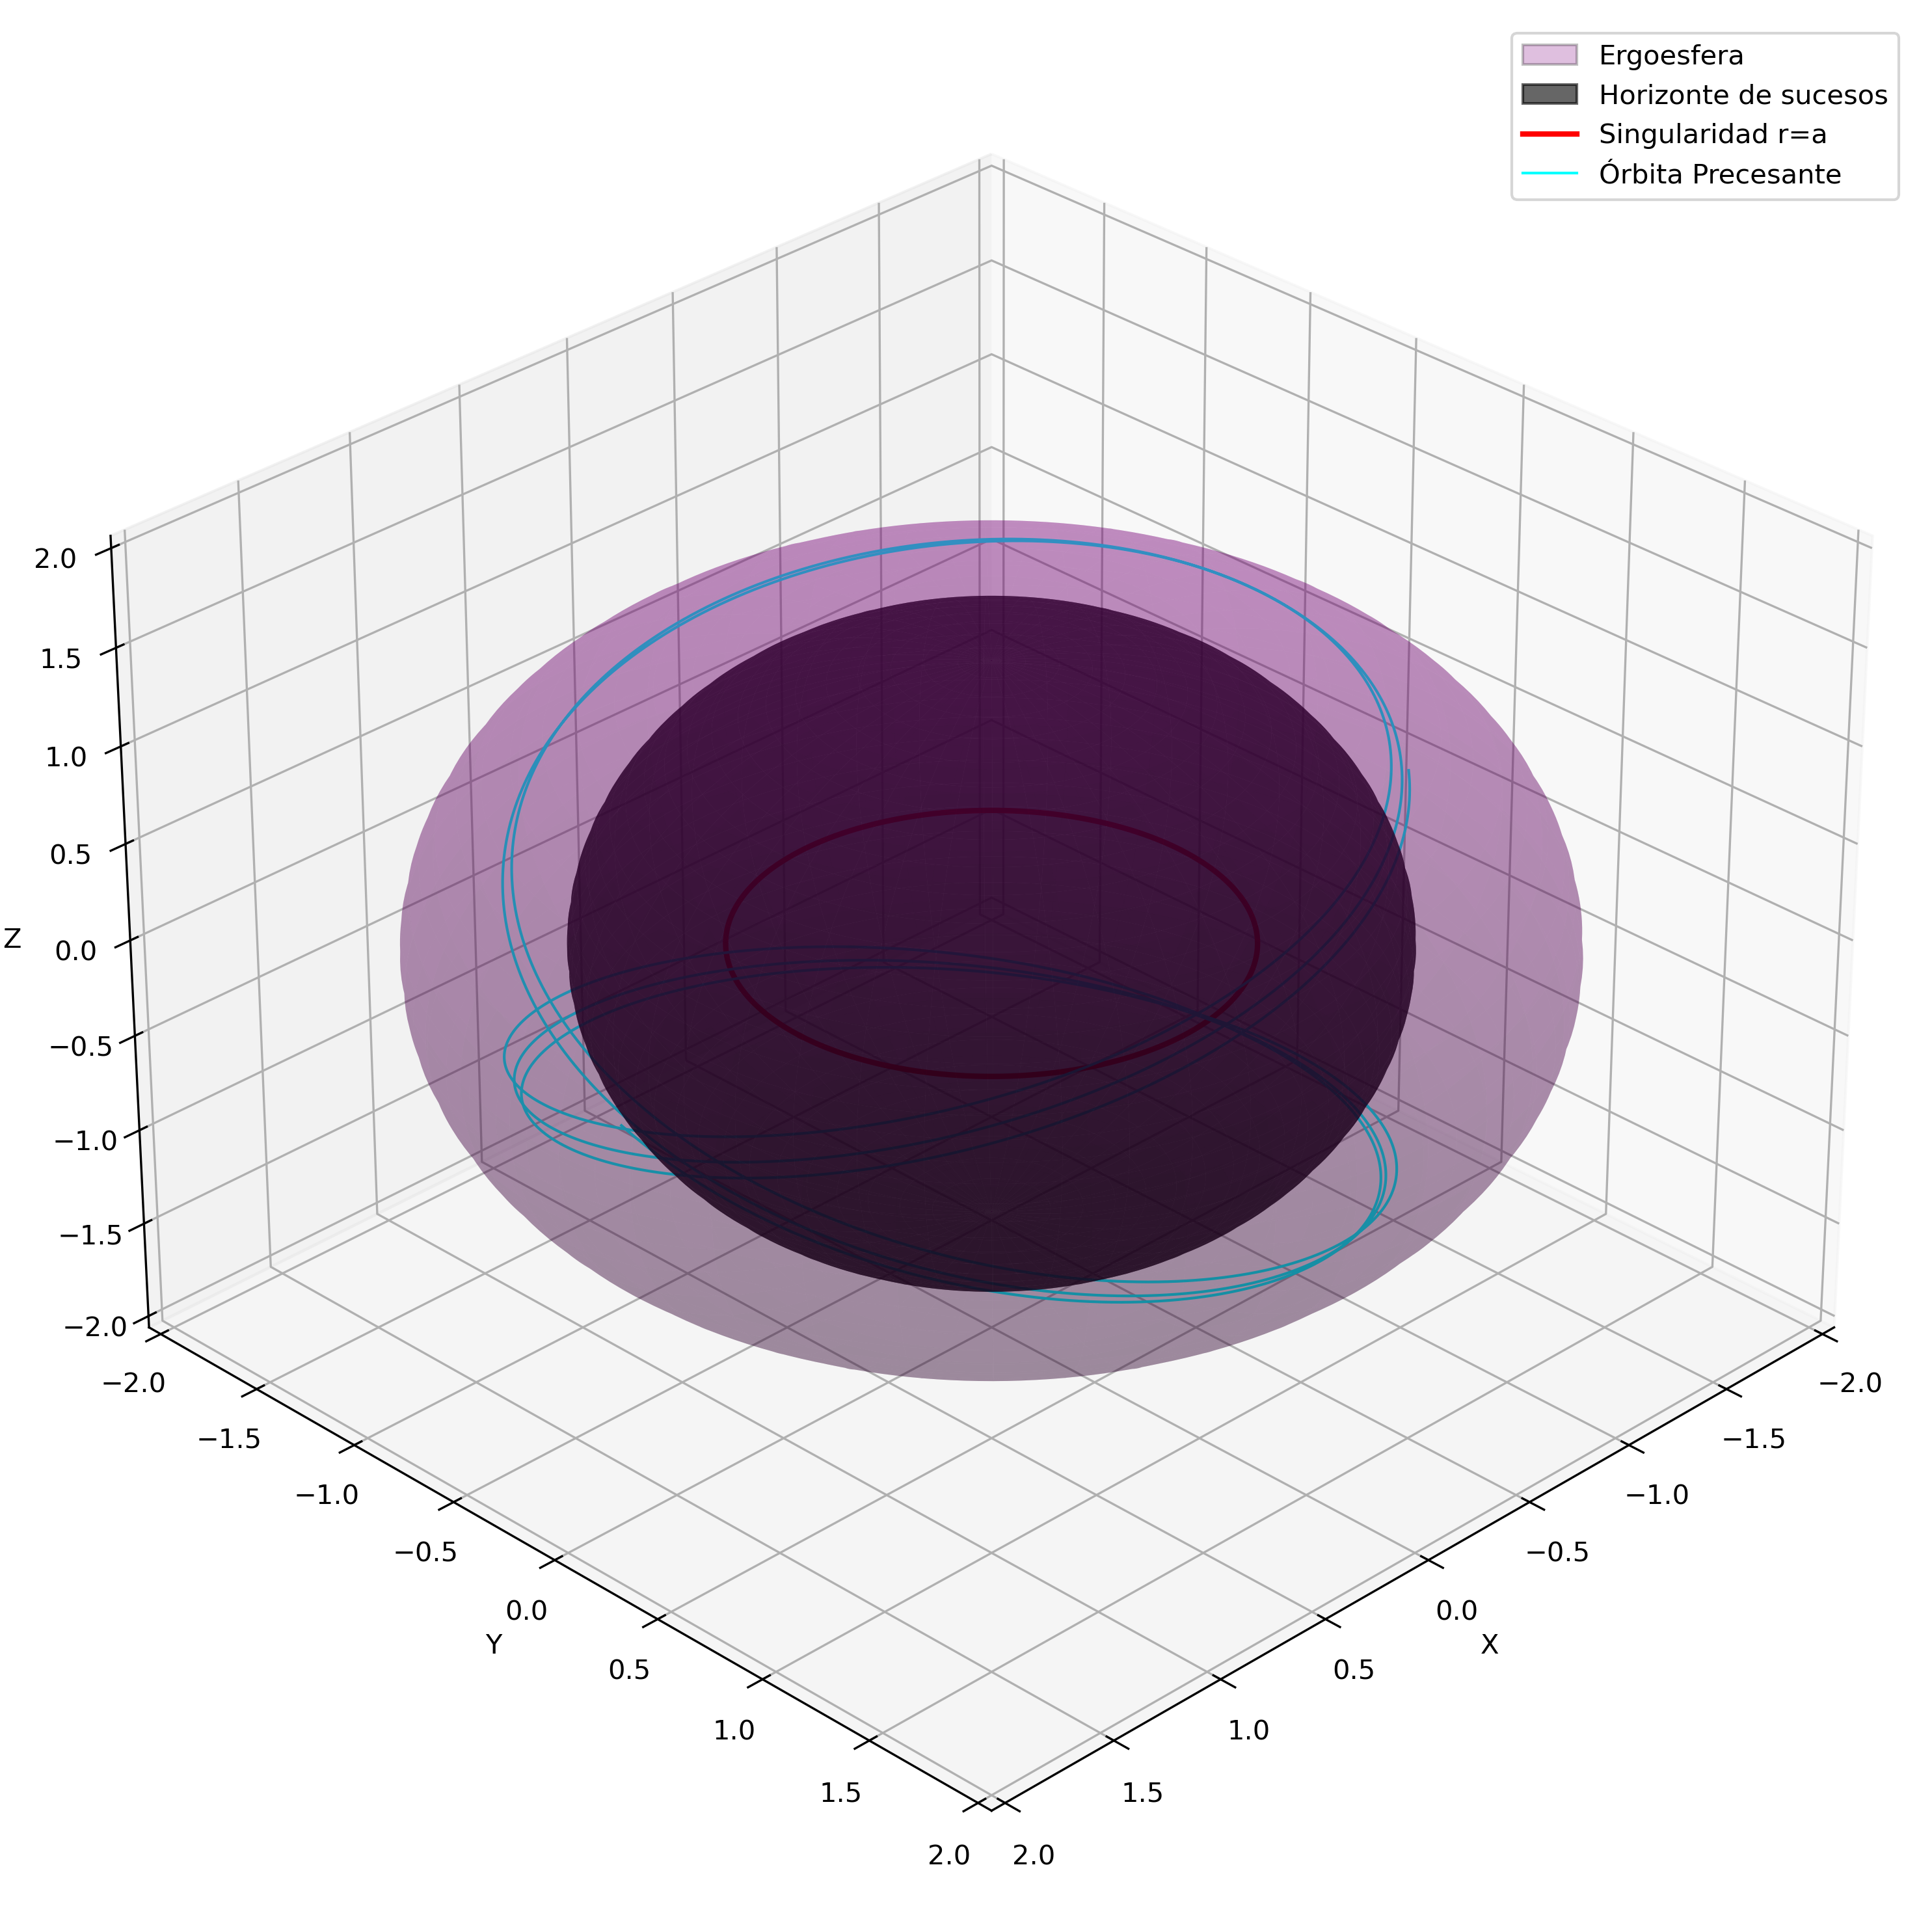
\includegraphics[width=0.95\textwidth]{AgujerosNegros/kerr/geodesics_plots/geodesica_circular_foton_r1,7179.png}
        \end{center}
        \caption{Geodésica circular de fotón en Kerr con $a = 0.9$, $m=1$ y $c=1$.}
        \label{fig:geodesica_circular_foton_r1,7179}
    \end{small}
\end{figure}
